\documentclass[12pt]{article}

\usepackage{amsmath, amsthm, amssymb, amsfonts}
\usepackage{derivative, cancel, hyperref, bookmark}
\usepackage[english]{babel}
\usepackage[Rejne]{fncychap}
\usepackage[utf8]{inputenc}
\usepackage[T1]{fontenc}
\usepackage{mathpazo}
\usepackage{caption, subcaption}
\usepackage[dvipsnames]{xcolor}
\usepackage{tcolorbox, color, soul}
\usepackage[a4paper, portrait, margin=1.5cm]{geometry}
\tcbuselibrary{theorems, skins, breakable}
\hypersetup{colorlinks=true, linkcolor=blue, filecolor=magenta, urlcolor=cyan}

\begin{document}

\begin{titlepage}
	\newcommand{\HRule}{\rule{\linewidth}{0.5mm}}
	\center
	
	% Headings
	\textsc{\Huge Systems and Control Engineering}\\[1.5cm]	
	\textsc{\LARGE\bfseries SC649: Embedded Controls and Robotics}\\[1cm] % Major heading
	
	% Title
	\HRule\\[0.4cm]	
	{\huge\bfseries Assignment 2}\\[0.2cm] % Title of your document
	\HRule\\[1.5cm]
	
	% Author(s)
	\begin{minipage}{0.4\textwidth}
		\begin{flushleft}
			\large
			\textit{Team}\\
			\textsc{Pranav Gupta} (\texttt{22B2179})\\
			\textsc{Rohan Mekala} (\texttt{22B2106})\\
			\textsc{Sahil Sudhakar} (\texttt{210010055})\\
		\end{flushleft}
	\end{minipage}
	~
	\begin{minipage}{0.4\textwidth}
		\begin{flushright}
			\large
			\textit{Instructor}\\
			\textsc{Prof. Leena Vachhani}\\
            \href{mailto:leena.vachhani@iitb.ac.in}{leena.vachhani@iitb.ac.in}
		\end{flushright}
	\end{minipage}
	
	% Logo
	\vfill\vfill\vfill
	\includegraphics[width=0.4\textwidth]{/home/pranav/Documents/LaTeX/SysCon/logo.png}\\[1cm]
	
	% Date
	\vfill\vfill
	{\LARGE \today}
	\vfill
	
\end{titlepage}

\pagebreak
\tableofcontents

\section*{Work Distribution}
\begin{enumerate}
	\item \textbf{Pranav Gupta} (\texttt{22B2179}): 
	\item \textbf{Rohan Mekala} (\texttt{22B2106}): 
	\item \textbf{Sahil Sudhakar} (\texttt{210010055}):
\end{enumerate}

\pagebreak

\section{Setup}
\begin{enumerate}
    \item We have used \texttt{IN3} and \texttt{IN4} pins of the \textbf{\textbf{L298N}} motor driver to provide differential inputs to the Arduino to rotate the motor in clockwise/anticlockwise direction.
    \item Since we have used \texttt{IN3} and \texttt{IN4}, we have used the \texttt{\texttt{ENB}} pin of the motor driver to provide power to the motor via the Arduino.
    \item \texttt{\texttt{C1}} and \texttt{\texttt{C2}} are the inputs that we receive from the encoder based on the direction of the motor(encoder) rotation.
\end{enumerate}

\begin{figure}[ht!]
    \centering
    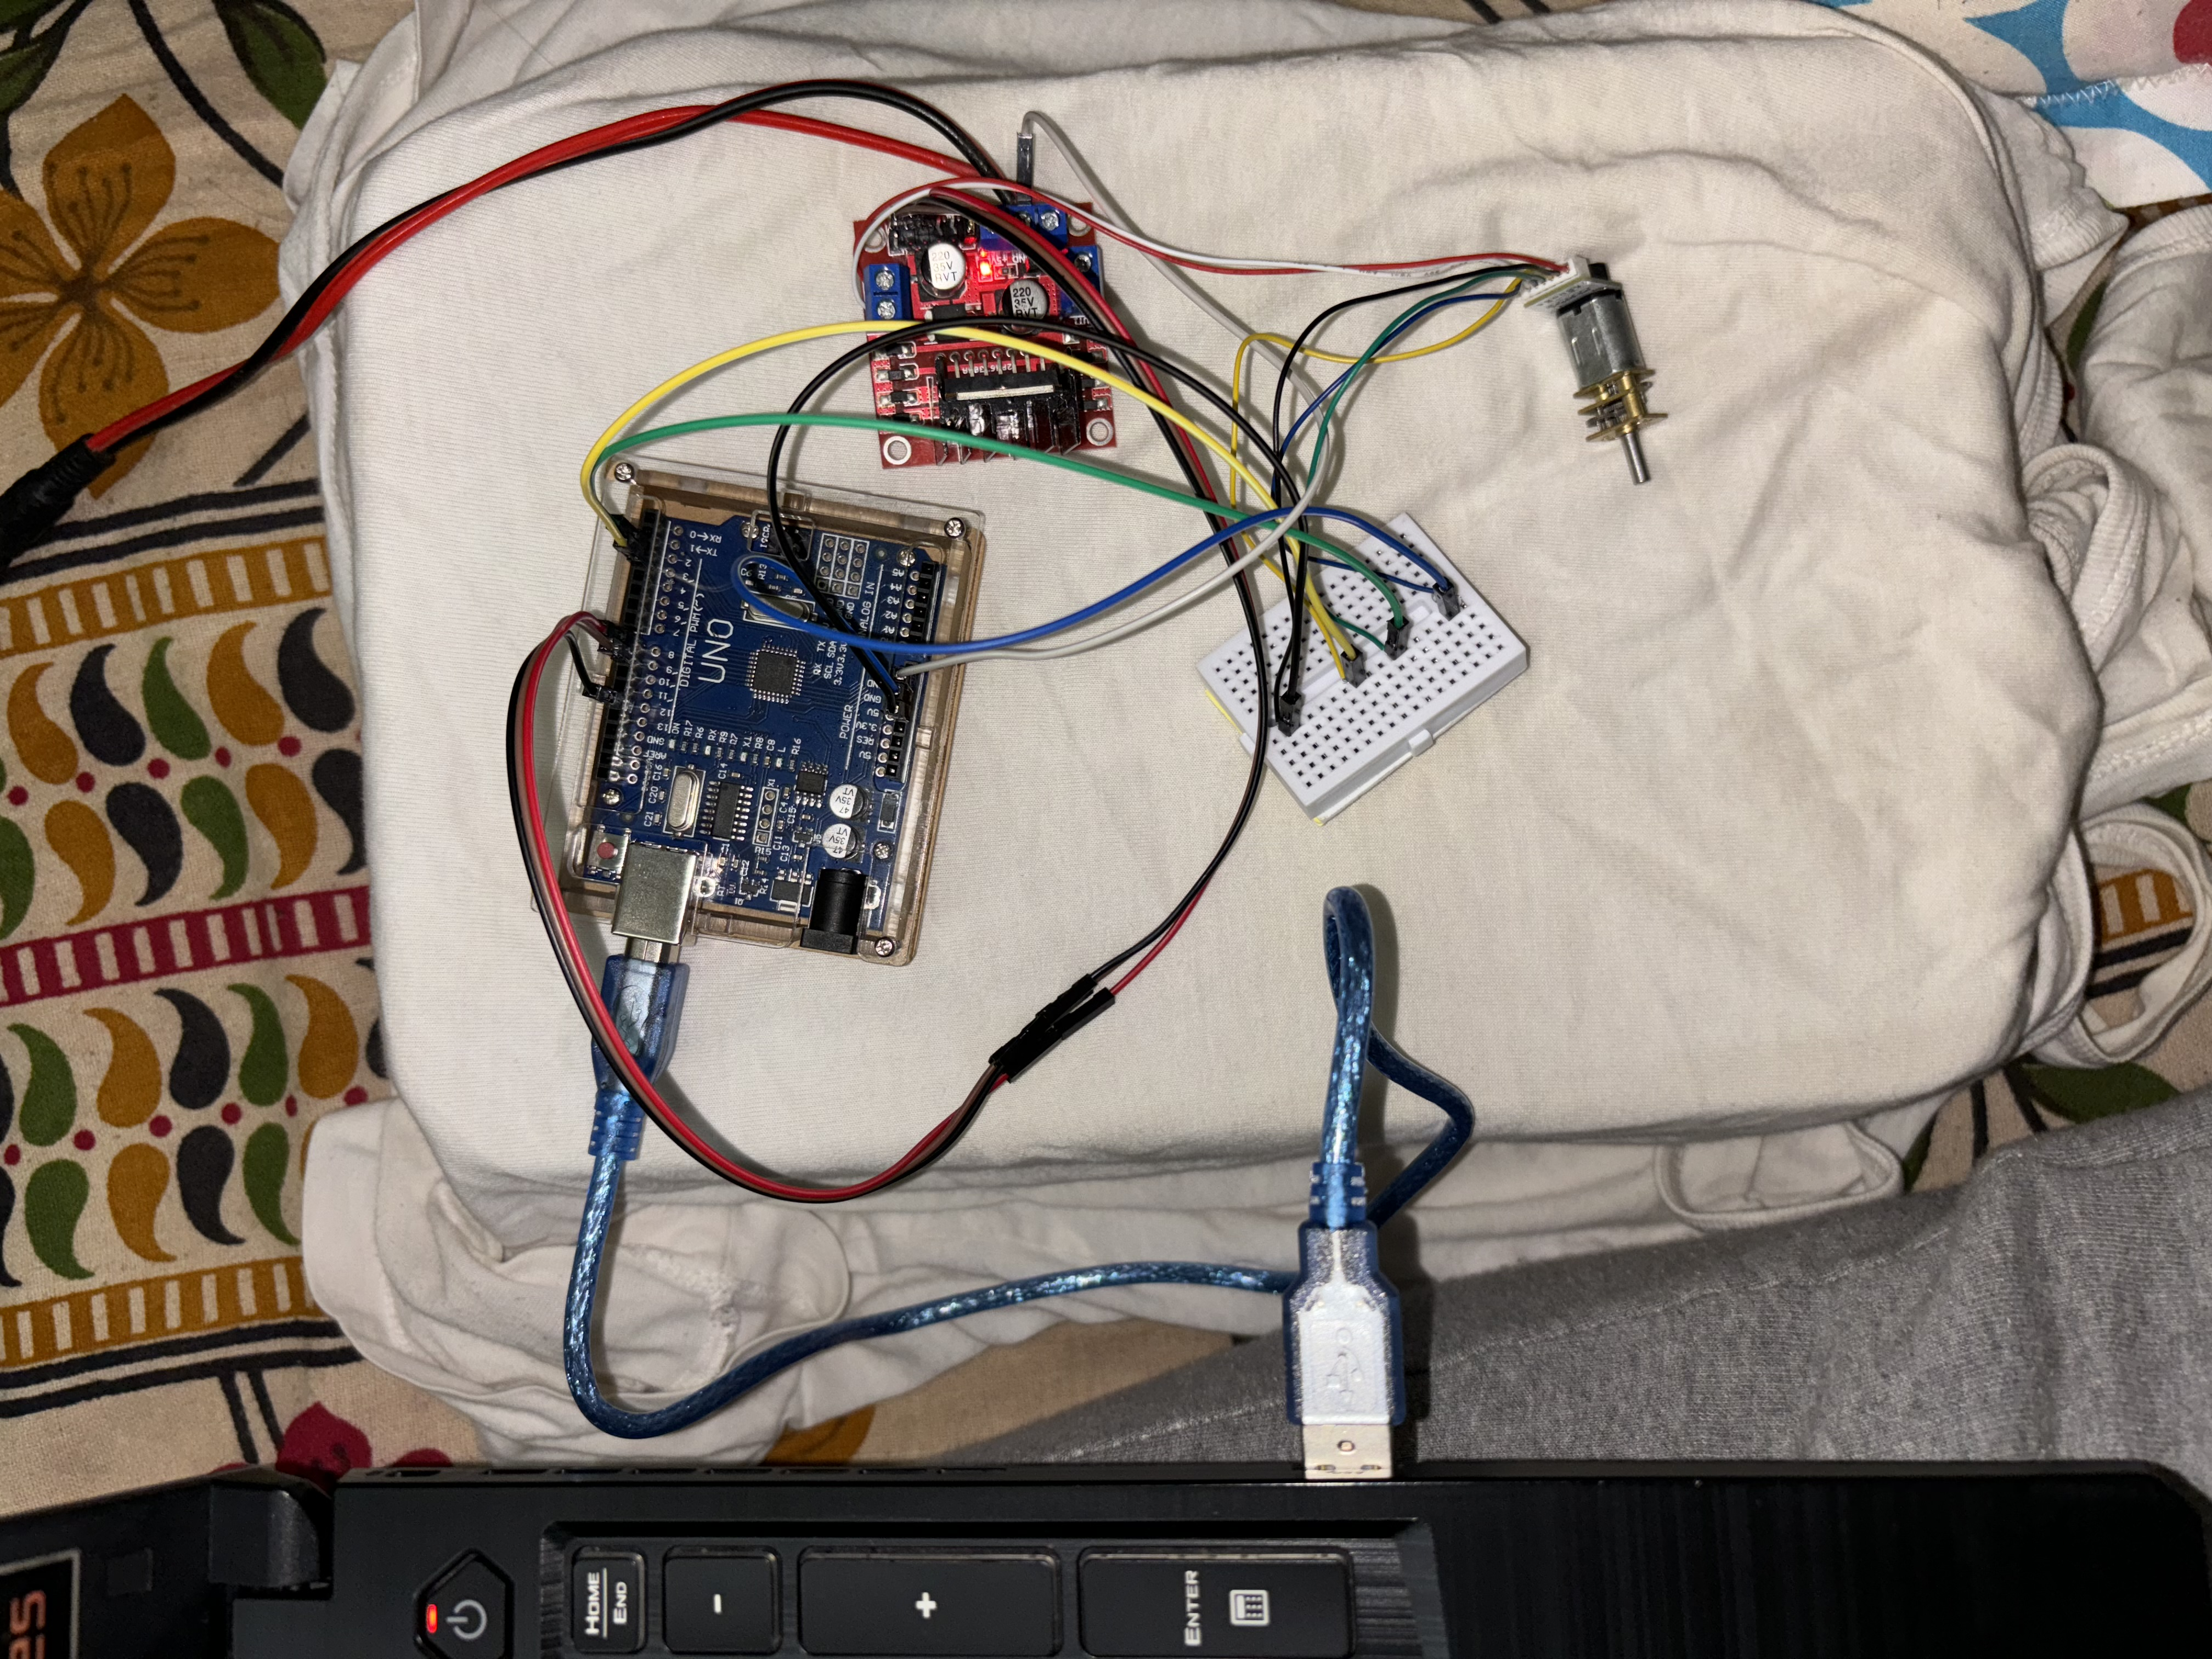
\includegraphics[width=0.75\textwidth]{images/setup.jpeg}
    \caption{photograph of setup}
\end{figure}

We have built upon the code from Assignment 1 to implement a \textit{Proportional Integral Derivative} (PID) controller on the DC motor's angular velocity (RPM). We have used the \texttt{C1-C2} encoder state pattern identification for the tick counter logic, as explained in Assignment 1. This is the underlying logic behind the \texttt{updateEncoderTicks()} function which is essential for the calculation of RPM. Another function which we have used from our original code is the \texttt{updateRPM()} function. Using the \texttt{micros()} function, we are able to allocate intervals of \texttt{N} microseconds to average the RPM over RPM by simply doing \texttt{(360/TPMR) * TPS * (1/60)} where \texttt{TPMR} \(\equiv\) Ticks Per Motor Rotation (experimentally we have found out to be 625) from our Assignment 1 conclusions and \texttt{TPS} \(\equiv\) ticks per second calculated using the tick counter logic over \texttt{N} microseconds. We have chosen \texttt{N} to be 10,000 \(\mu\)s \(=\) 0.1 seconds in our code. We have used \texttt{if(Serial.available() != 0)} function to detect user input RPM from the Arduino IDE serial monitor (without halting the program logic) which was the case with using \texttt{while(Serial.available() != 0)}. We have noticed an error that once an RPM value is input by the user, the subsequent iteration of \texttt{void loop()}, the setpoint RPM is reset to 0, which we fixed by implementing a logic which retain the previously entered non-zero setpoint RPM in case of no user input.

\section{PID Implementation}

Then we simply single integrated \texttt{duty\_d} to get the duty cycle (\texttt{duty}) by multiplying with \texttt{dt}. We have used the \texttt{loopT} variable to track the runtime of the latest \texttt{void loop()} in microseconds using inbuilt function \texttt{micros()} and \texttt{dt} is simply \texttt{loopT/1000000} to get the value in seconds.

\subsection*{Proportional error logic}
The \texttt{updateRPM()} function helps us to instantaneously update \texttt{currRPM} which is subtracted from the \texttt{setpRPM} to get the proportional error term.

\subsection{Integral error logic}
For the integral error term \texttt{e\_I}, we have simply integrated the proportional error term \texttt{e\_P}. Here, we have defined \texttt{e\_P} as an array to resolve the following issue: \texttt{e\_I} retains memory of the errors during transient response and this error is then propagated further in as we approach steady state due to integration. So, to remove this initial error which is retained in \texttt{e\_I}, we have defined a memory size variable \texttt{MEMSZ} (initialised to 25 in our case) which is essentially the length of this array. At any given iteration of \texttt{void loop()}, the computed \texttt{e\_I} will only retain the integral over the last 25 error integrals to prevent steady state error due to earlier errors. At the end of 25 iterations of the void loop, \texttt{idx} (which is the index variable for \texttt{e\_P[]}) and \texttt{e\_I} are reset to 0, to initiate overwriting over the oldest errors and replace them with the latest, one by one. That is why we first subtract the old error at an index from \texttt{e\_I} at the index before overwriting it with the current proportional error, and integrate the same into \texttt{e\_I}. 

\subsection*{Derivative error logic}
For the \texttt{e\_D} term, we simply calculated the difference between the current RPM (\texttt{currRPM}) using the \texttt{updateRPM()} logic and the previous RPM (\texttt{prevRPM}) which we stored from the last iteration of void loop() and divided by \texttt{dt} to get the derivative of the error. We have clipped the duty cycle value that we have computed using the control law between -255 and 255 to \texttt{analogWrite} to \texttt{ENB}.

\subsection{Manual PWM logic}
For manually changing the PWM frequency, we have defined the variable \texttt{pwmTmicros} which denotes the time period for manual pwm in microseconds.The \texttt{t\_on} time, for which we have to \texttt{digitalWrite} HIGH to ENB, simply becomes \texttt{pwmTmicros*(abs(duty)/255)} and the \texttt{t\_off} time, for which we have to digitalWrite LOW to ENB, is then \texttt{pwmTmicros*(1-abs(duty)/255)}.

\pagebreak

\section{Questions \& Answers}

\subsection{Question 1}
What is the effect of changing the values of PID gains, $K_P$, $K_I$ and $K_D$ on the output speed?

\subsubsection{Varying $K_D$}

\begin{figure}[h]
    \centering
    \begin{subfigure}{.49\textwidth}
        \centering
        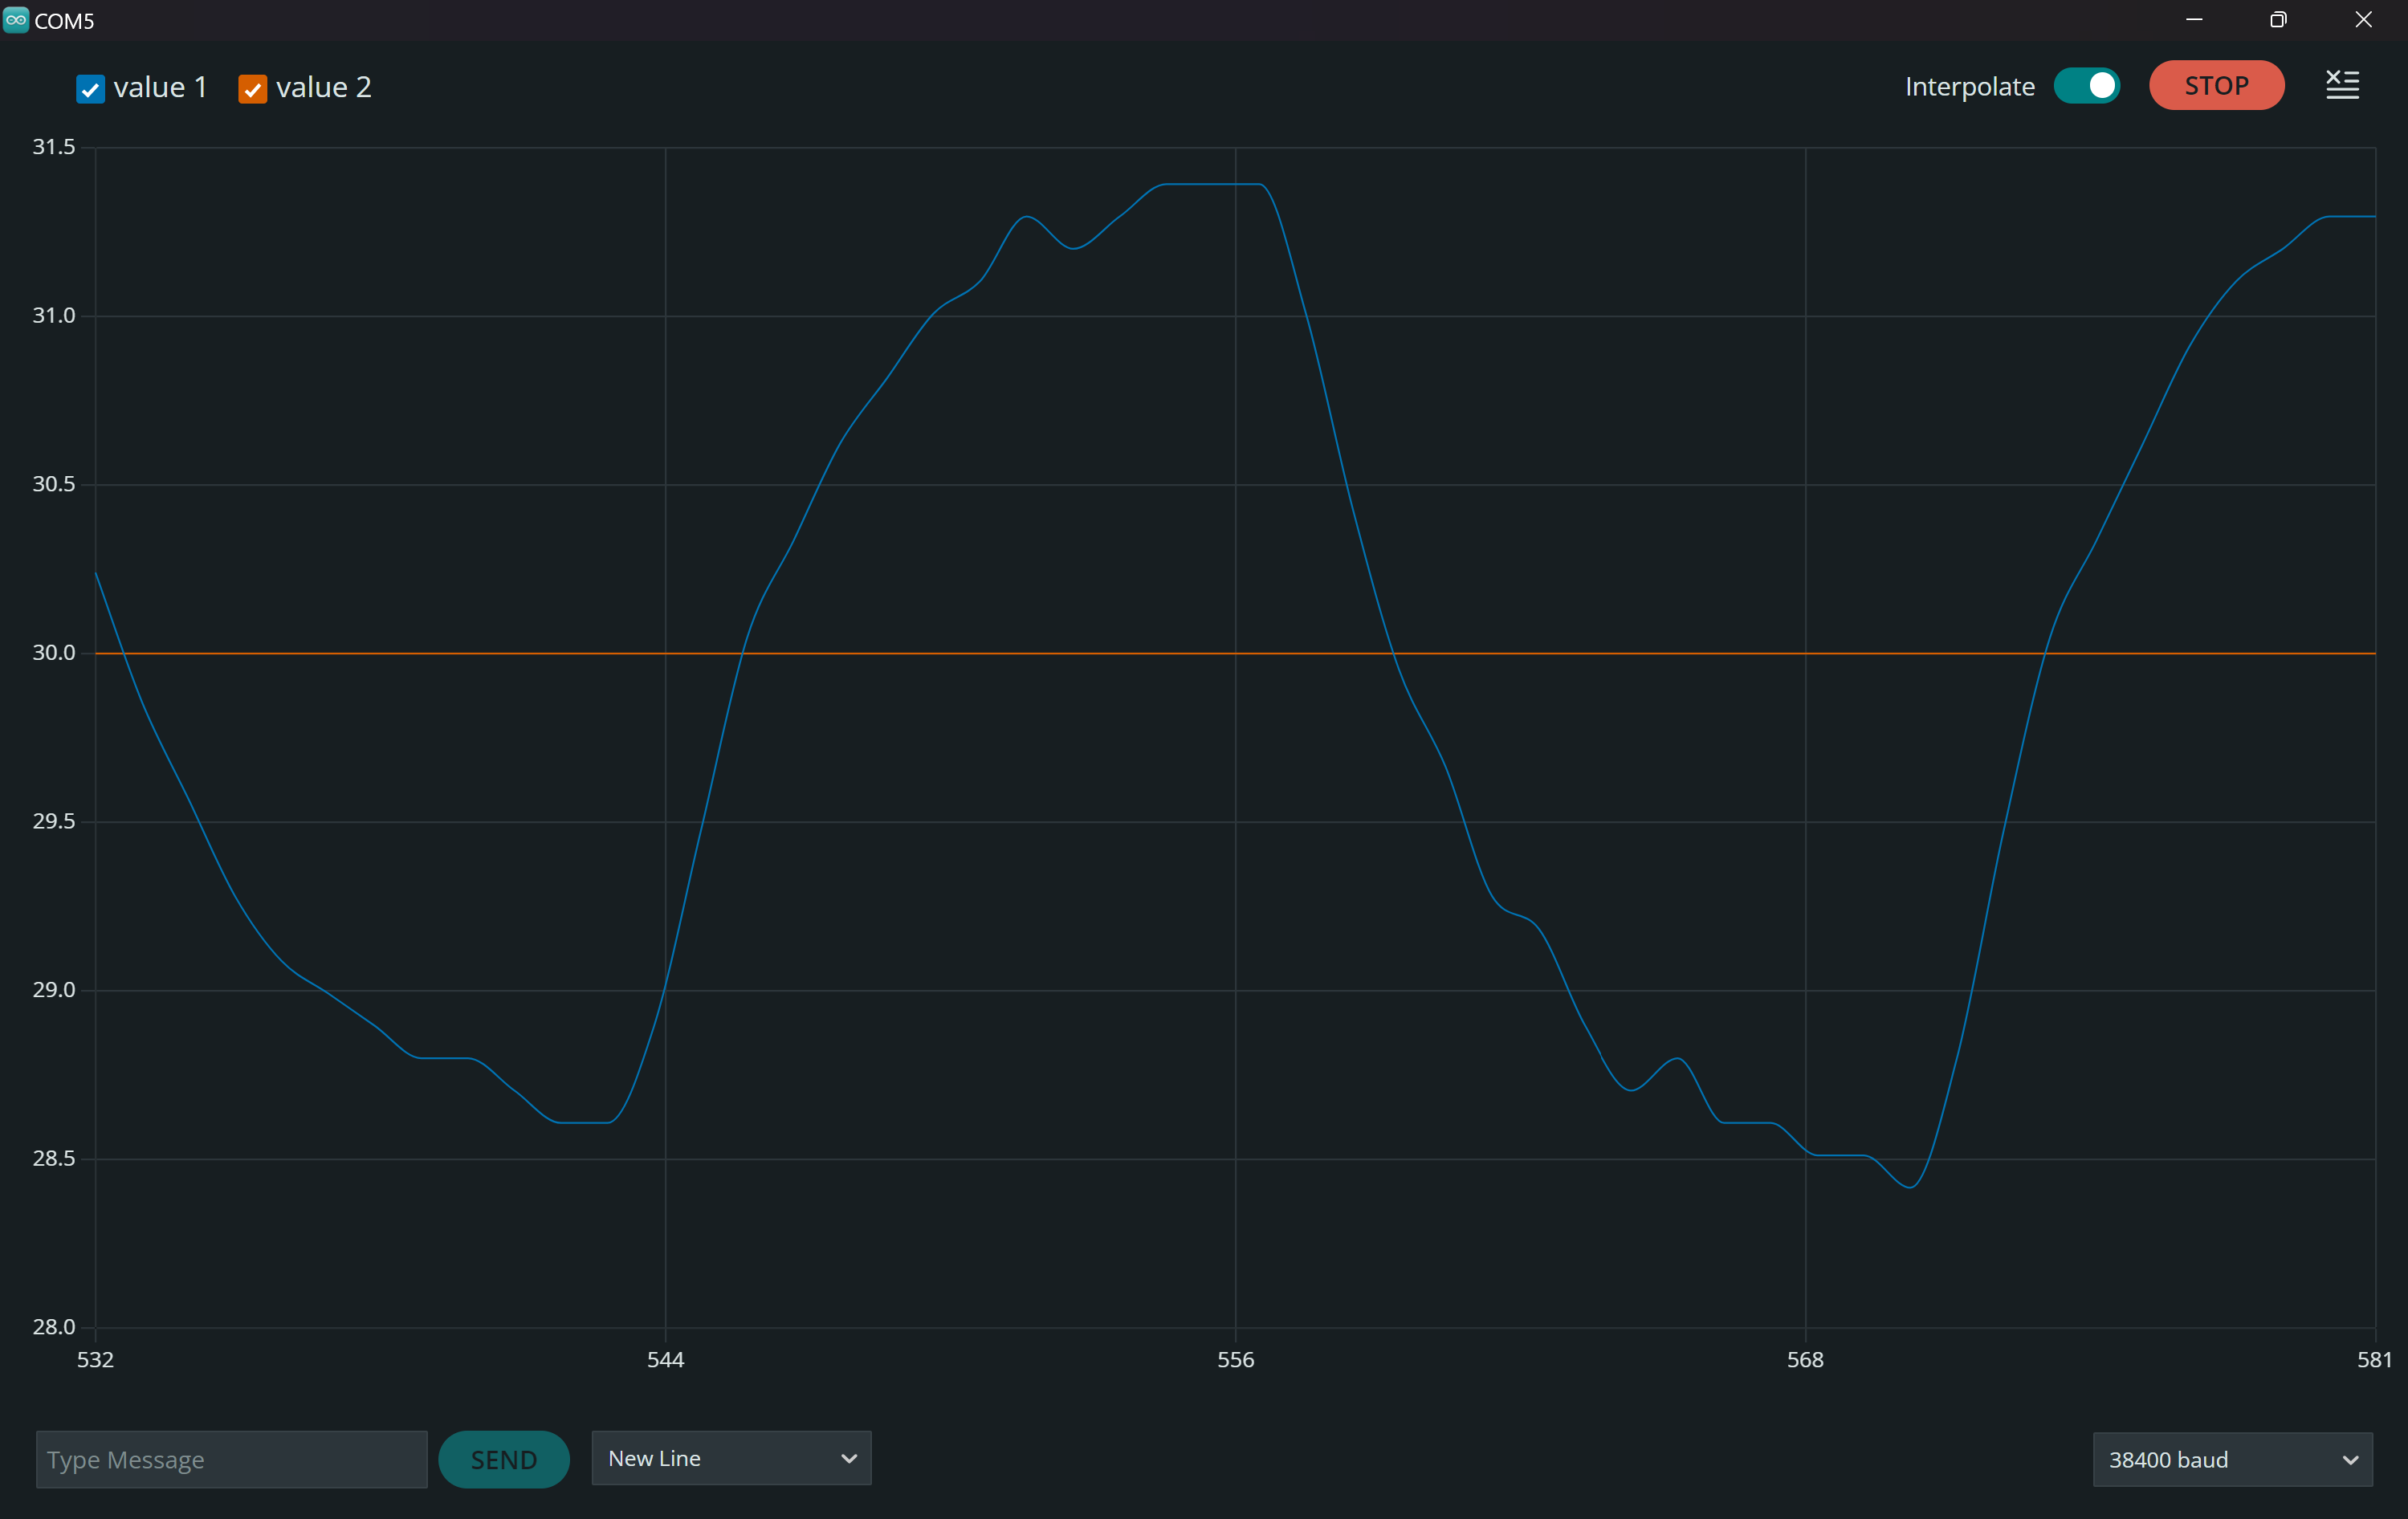
\includegraphics[width=0.95\linewidth]{images/q1/10_10_0.05.png}
		\caption{$K_D=0.05$}
    \end{subfigure}
    \begin{subfigure}{.49\textwidth}
        \centering
        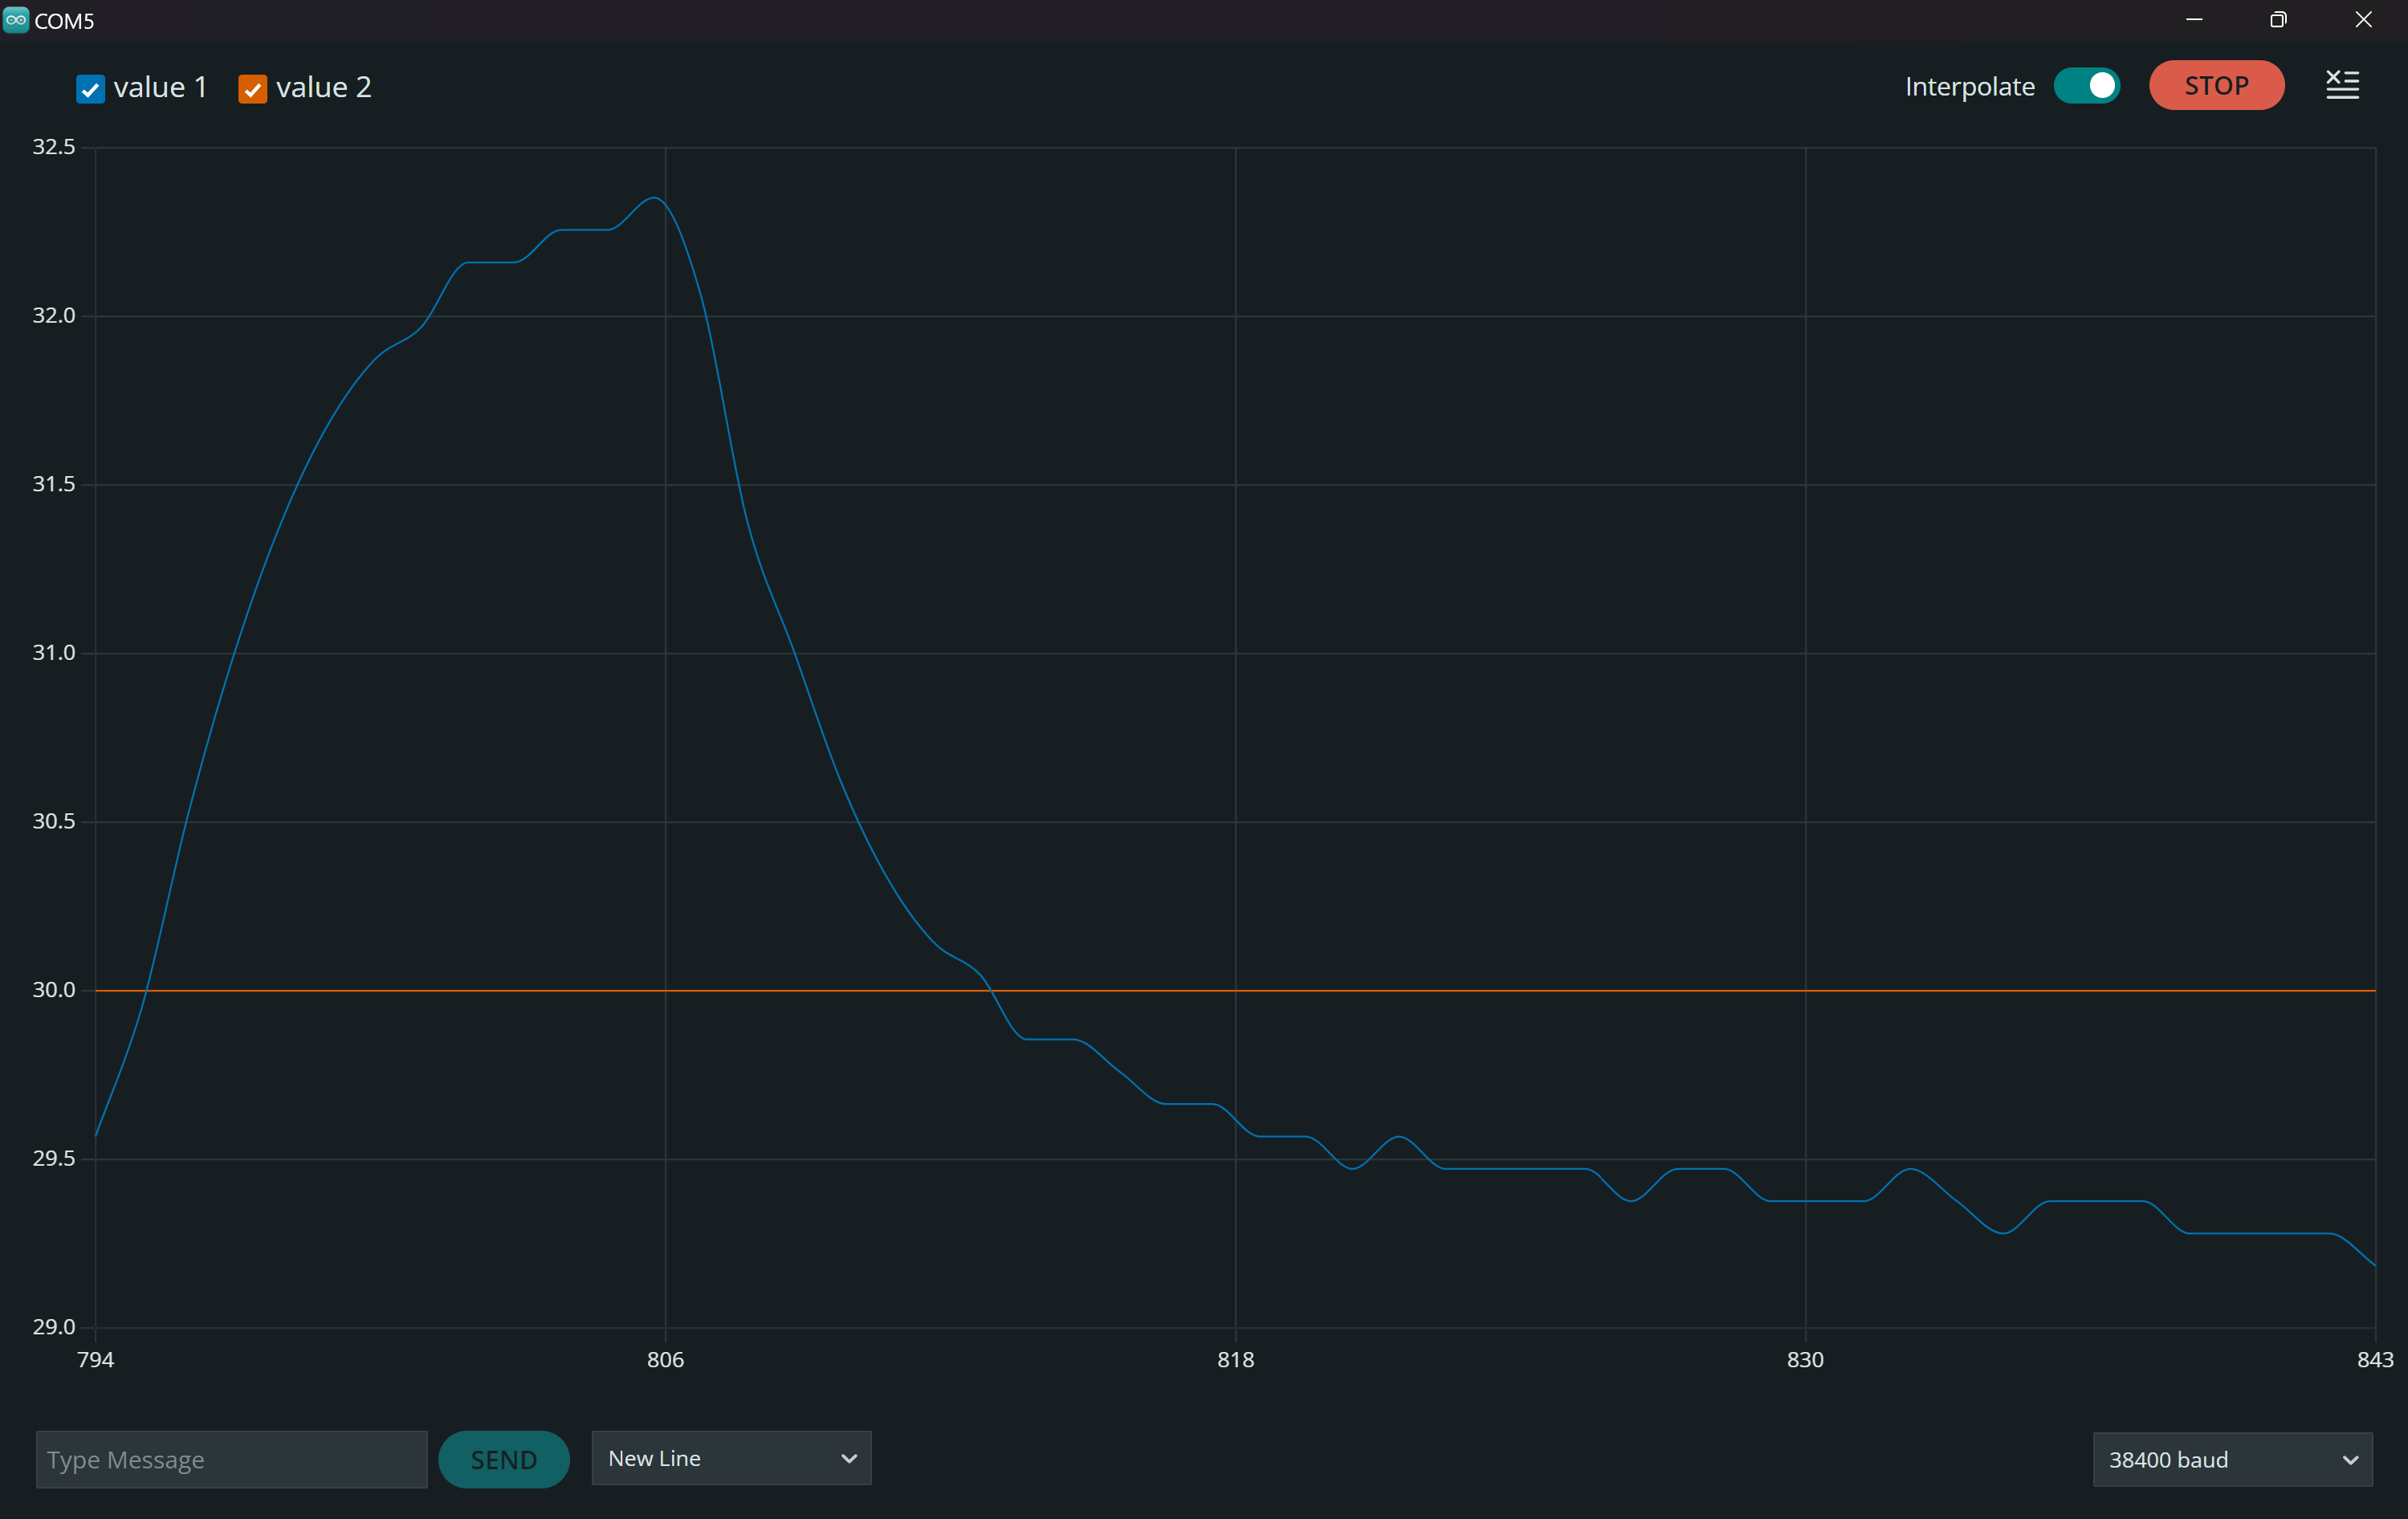
\includegraphics[width=0.95\linewidth]{images/q1/10_10_0.1.png} 
		\caption{$K_D=0.1$}
    \end{subfigure}
	\begin{subfigure}{.49\textwidth}
        \centering
        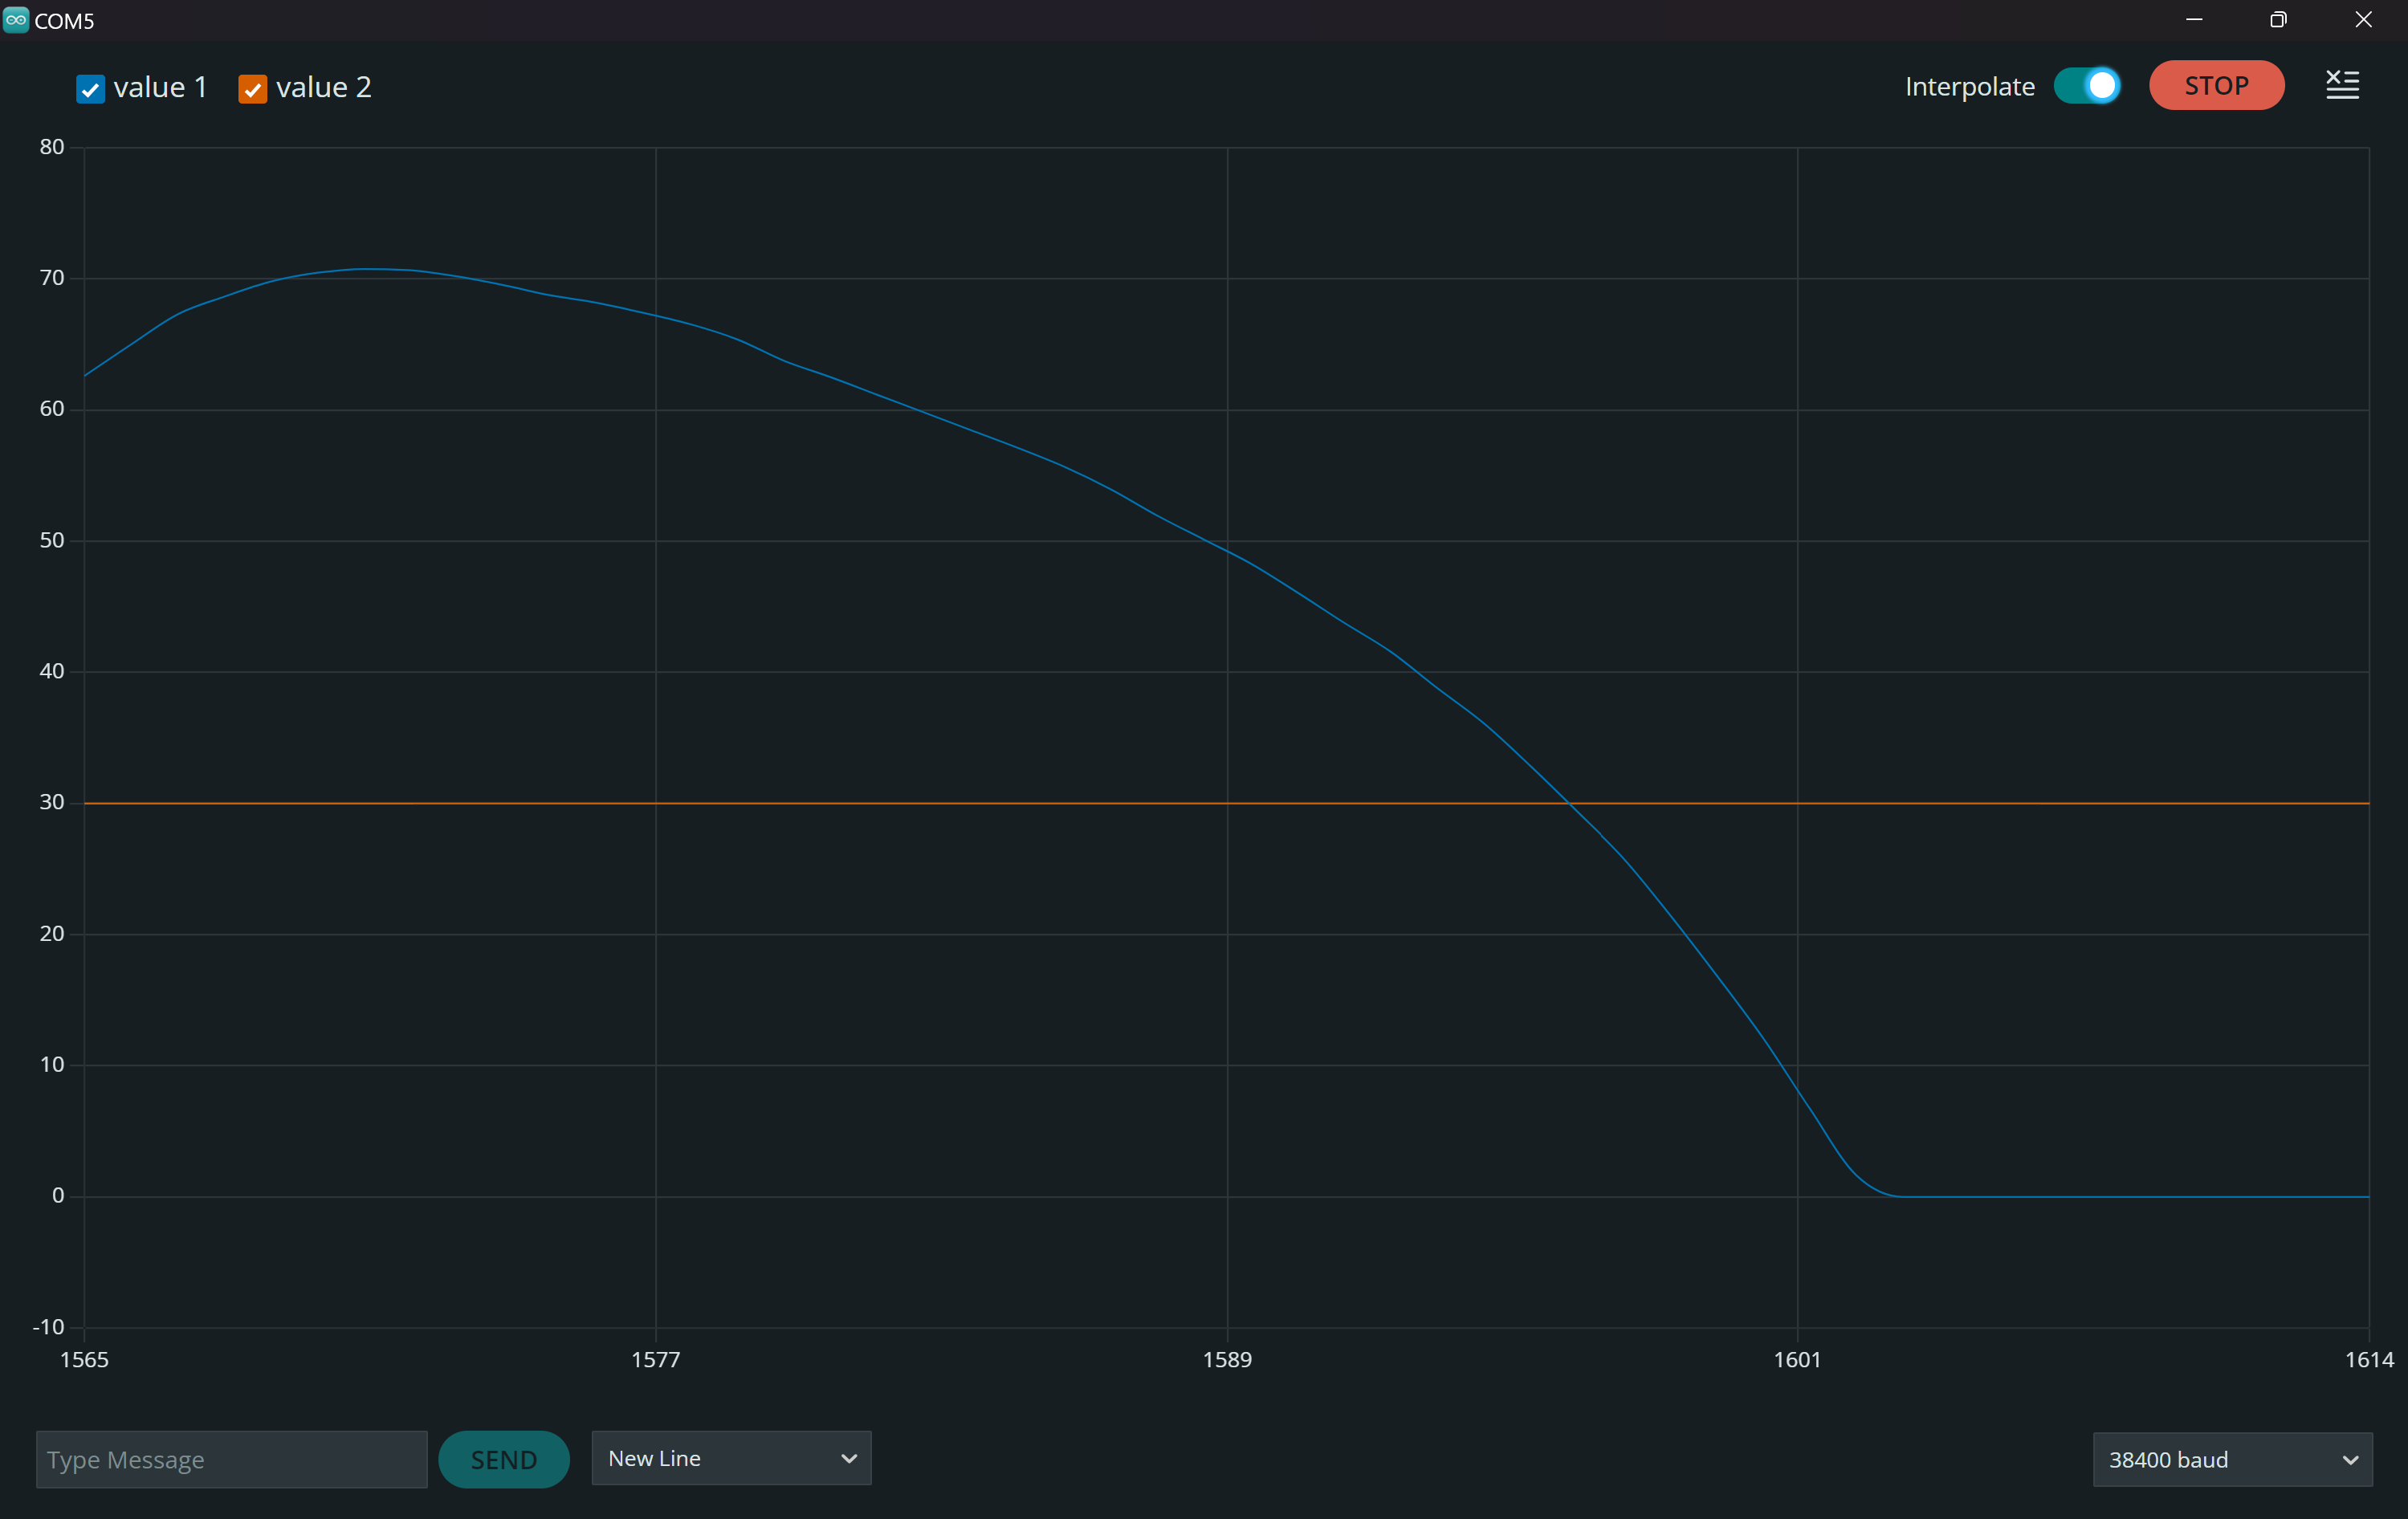
\includegraphics[width=0.95\linewidth]{images/q1/10_10_0.5.png}
		\caption{$K_D=0.5$}
    \end{subfigure}
    \begin{subfigure}{.49\textwidth}
        \centering
        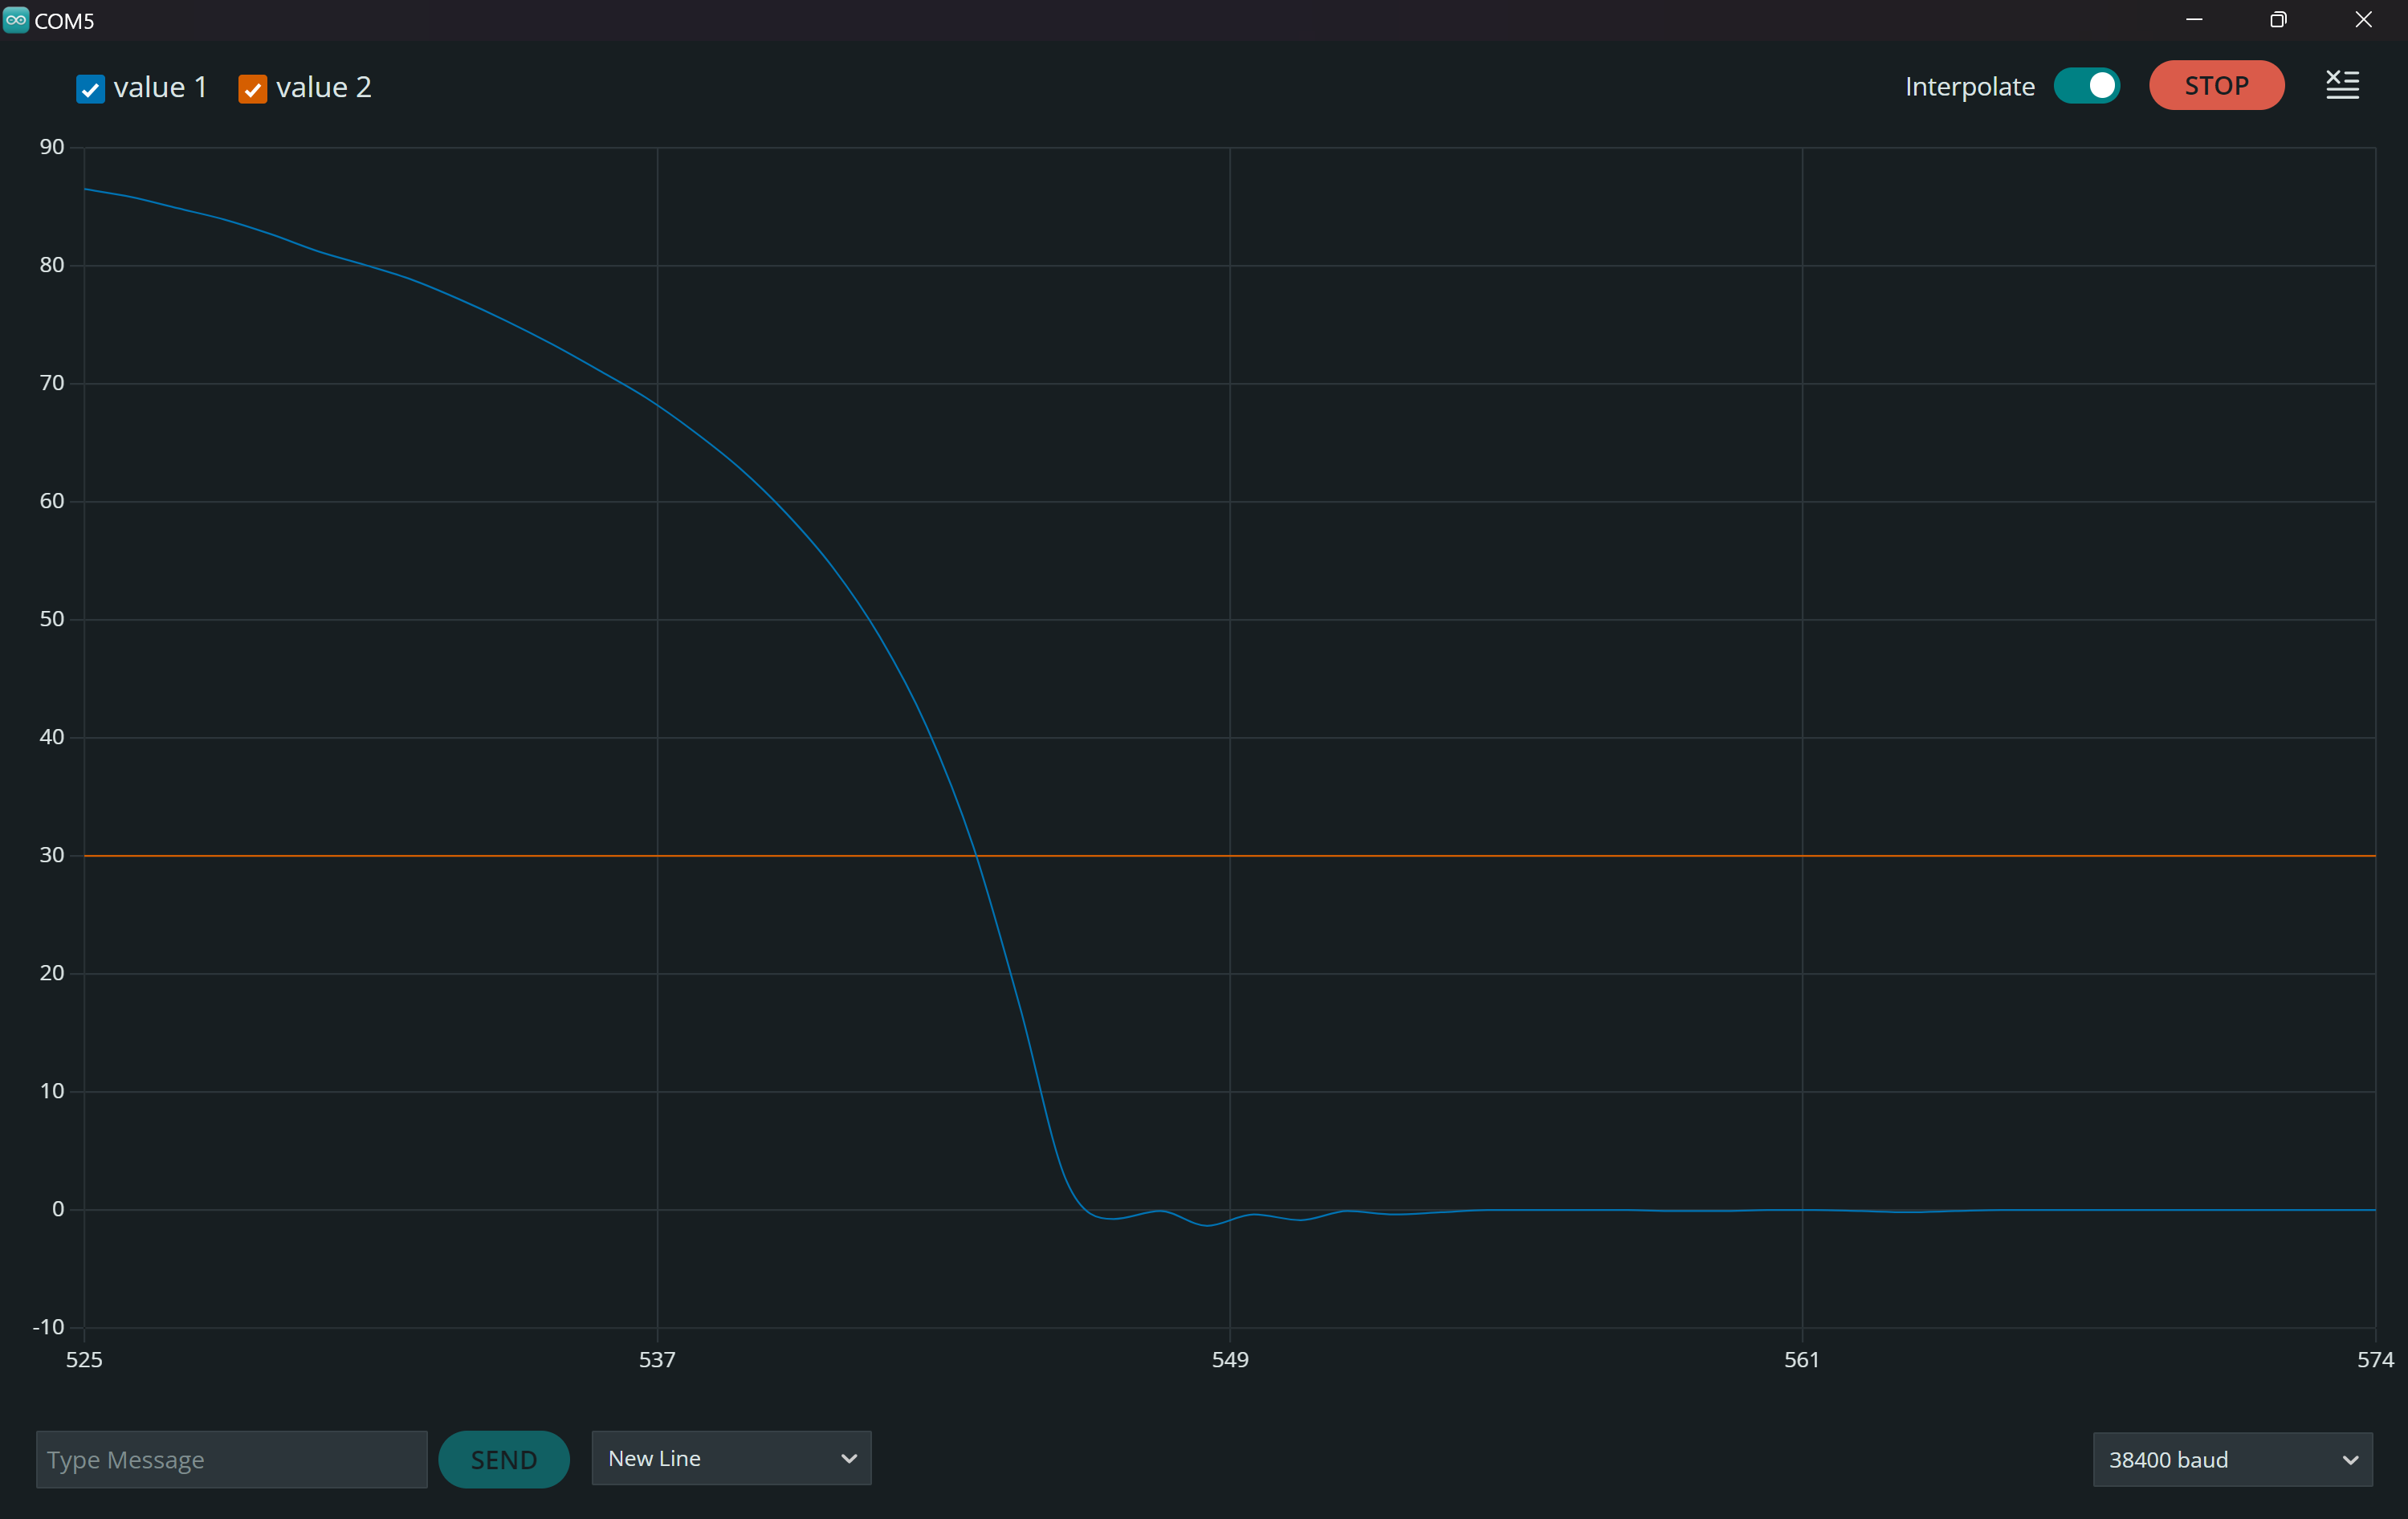
\includegraphics[width=0.95\linewidth]{images/q1/10_10_1.png} 
		\caption{$K_D=1$}
    \end{subfigure}
    \caption{transient responses for $K_P=10$, $K_I=10$ and various values of $K_D$}
\end{figure}

Based on the observations of using the $K_D$ term, we can clearly observe that the derivative error term is detrimental to the system response as the $K_D$ term amplifies the noise in the data and it would only work with filtered data without any noise. Therefore, we will not be using the derivative term for the rest of the questions to get a stable and converging system response.

\pagebreak

\subsubsection{Varying $K_P$}

\begin{figure}[h]
    \centering
    \begin{subfigure}{.44\textwidth}
        \centering
        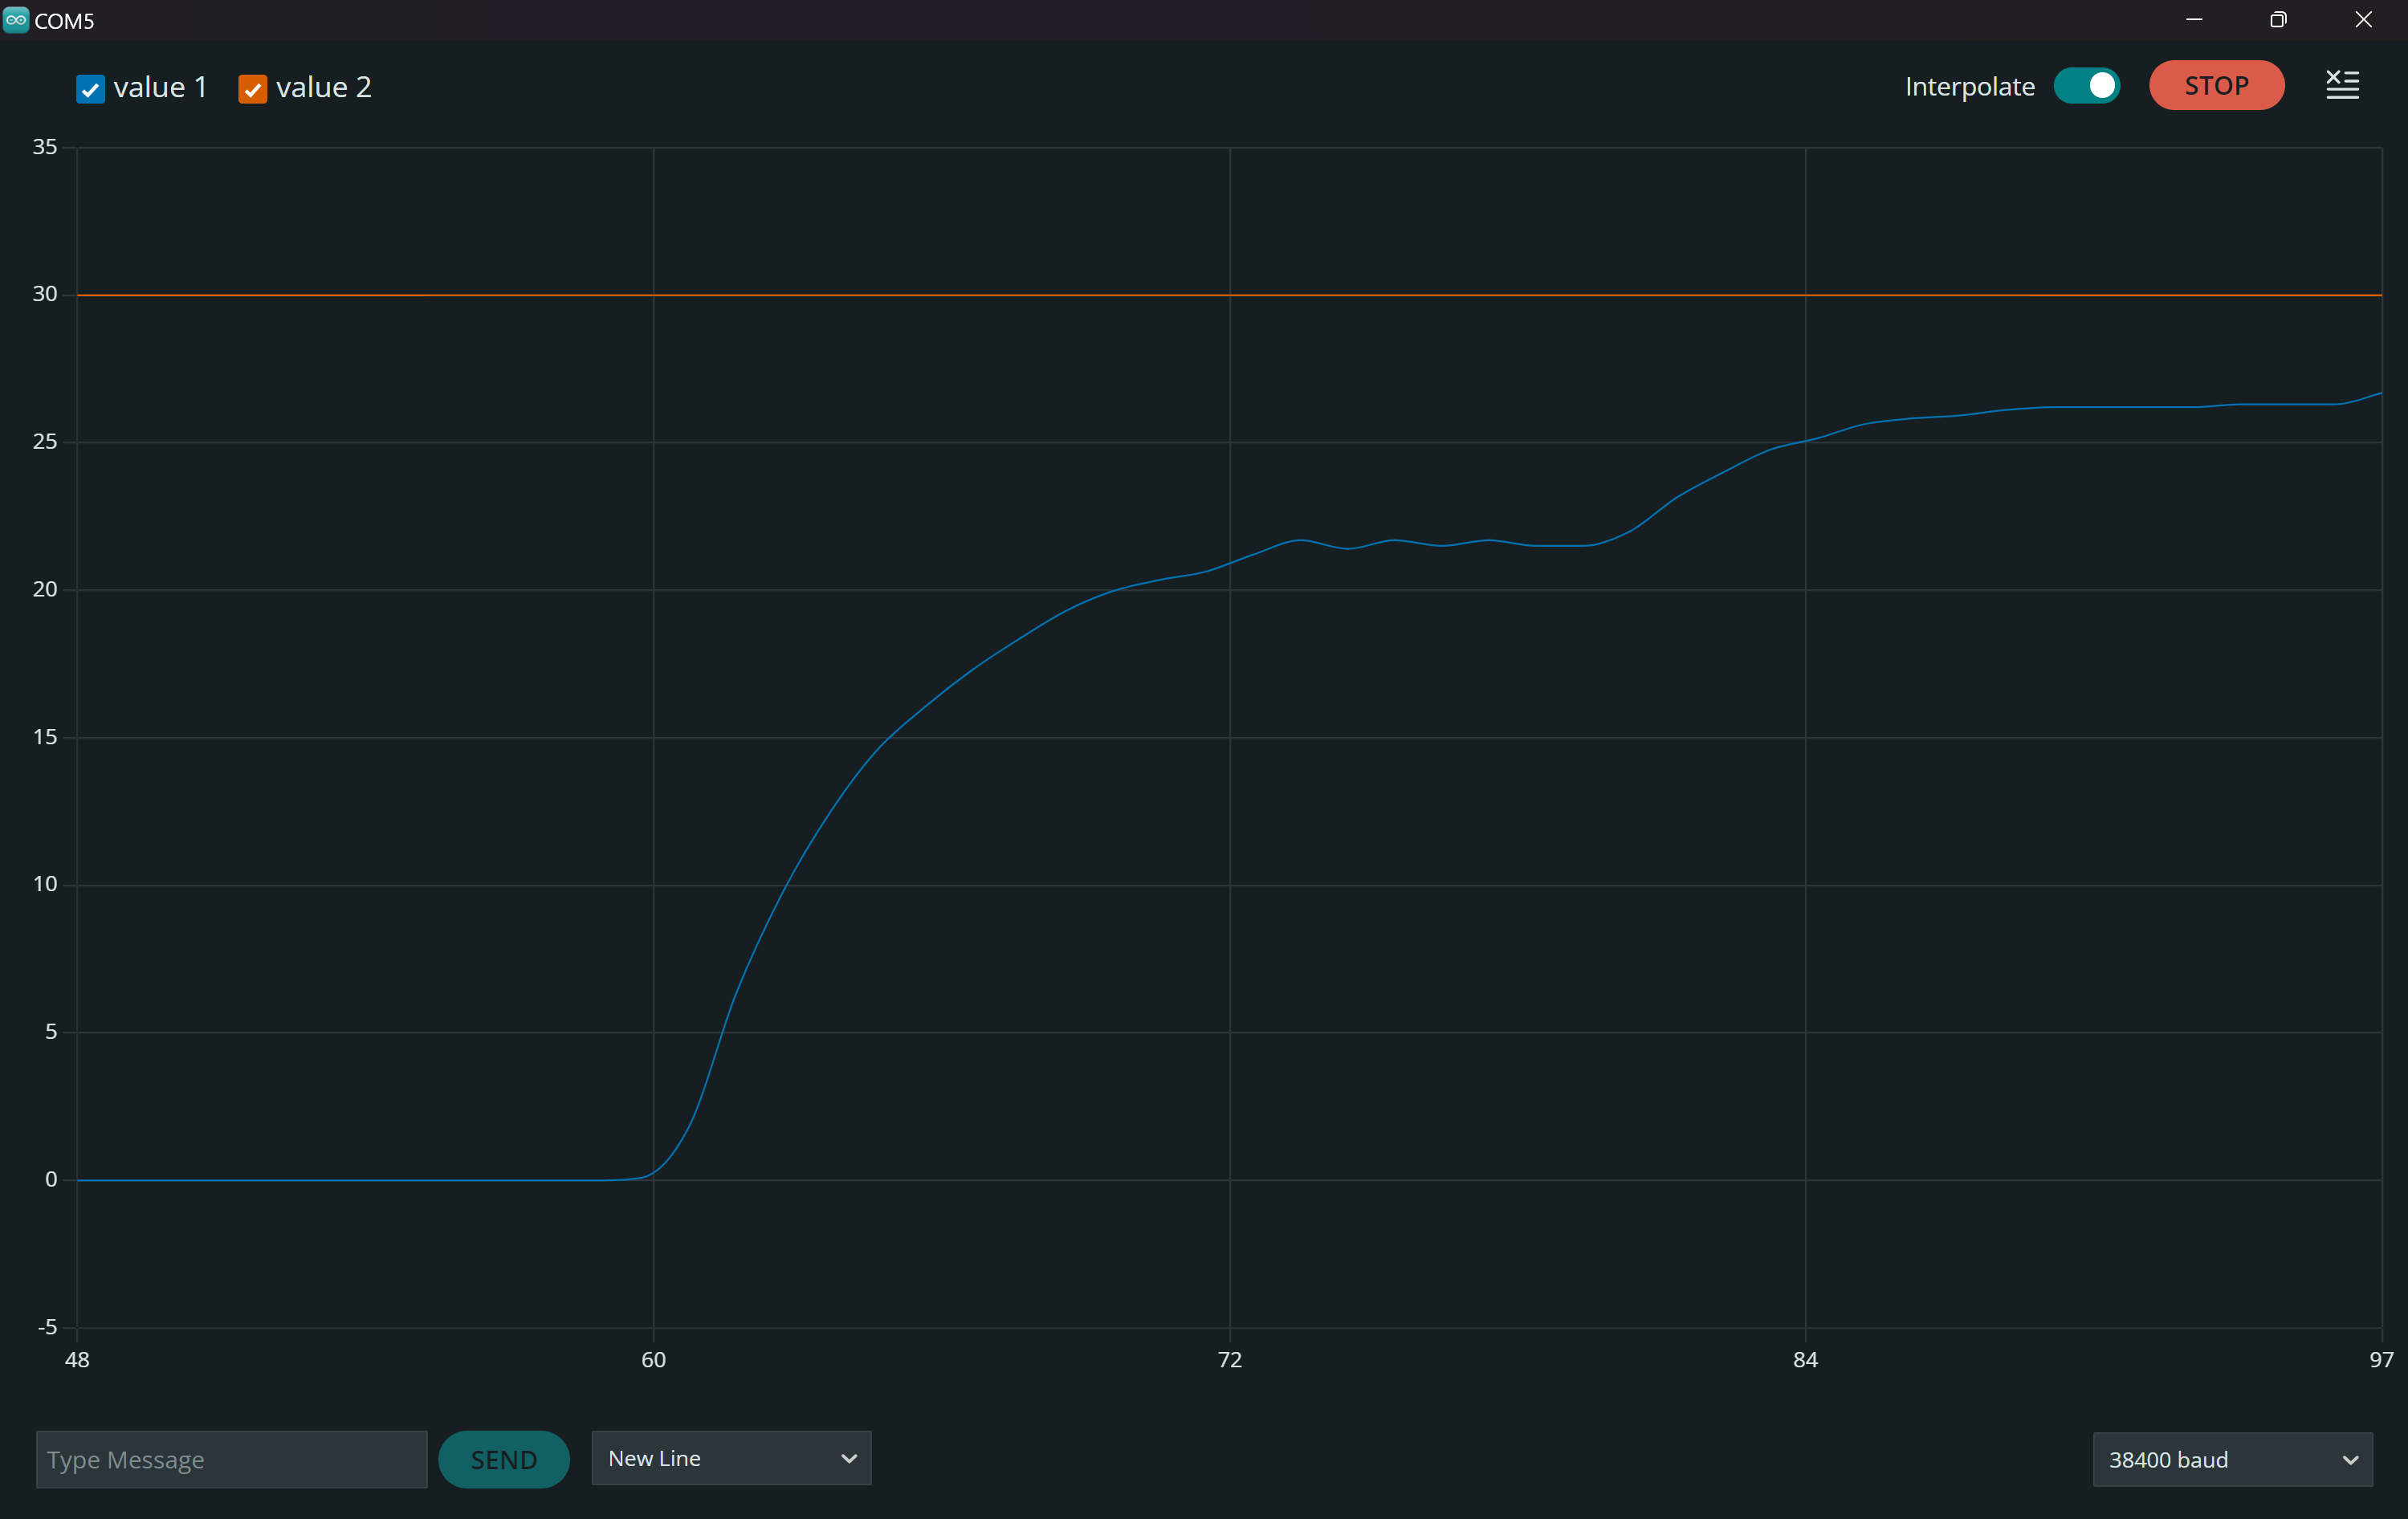
\includegraphics[width=0.95\linewidth]{images/q1/Transient_10_10_0.png}
		\caption{transient response}
    \end{subfigure}
    \begin{subfigure}{.44\textwidth}
        \centering
        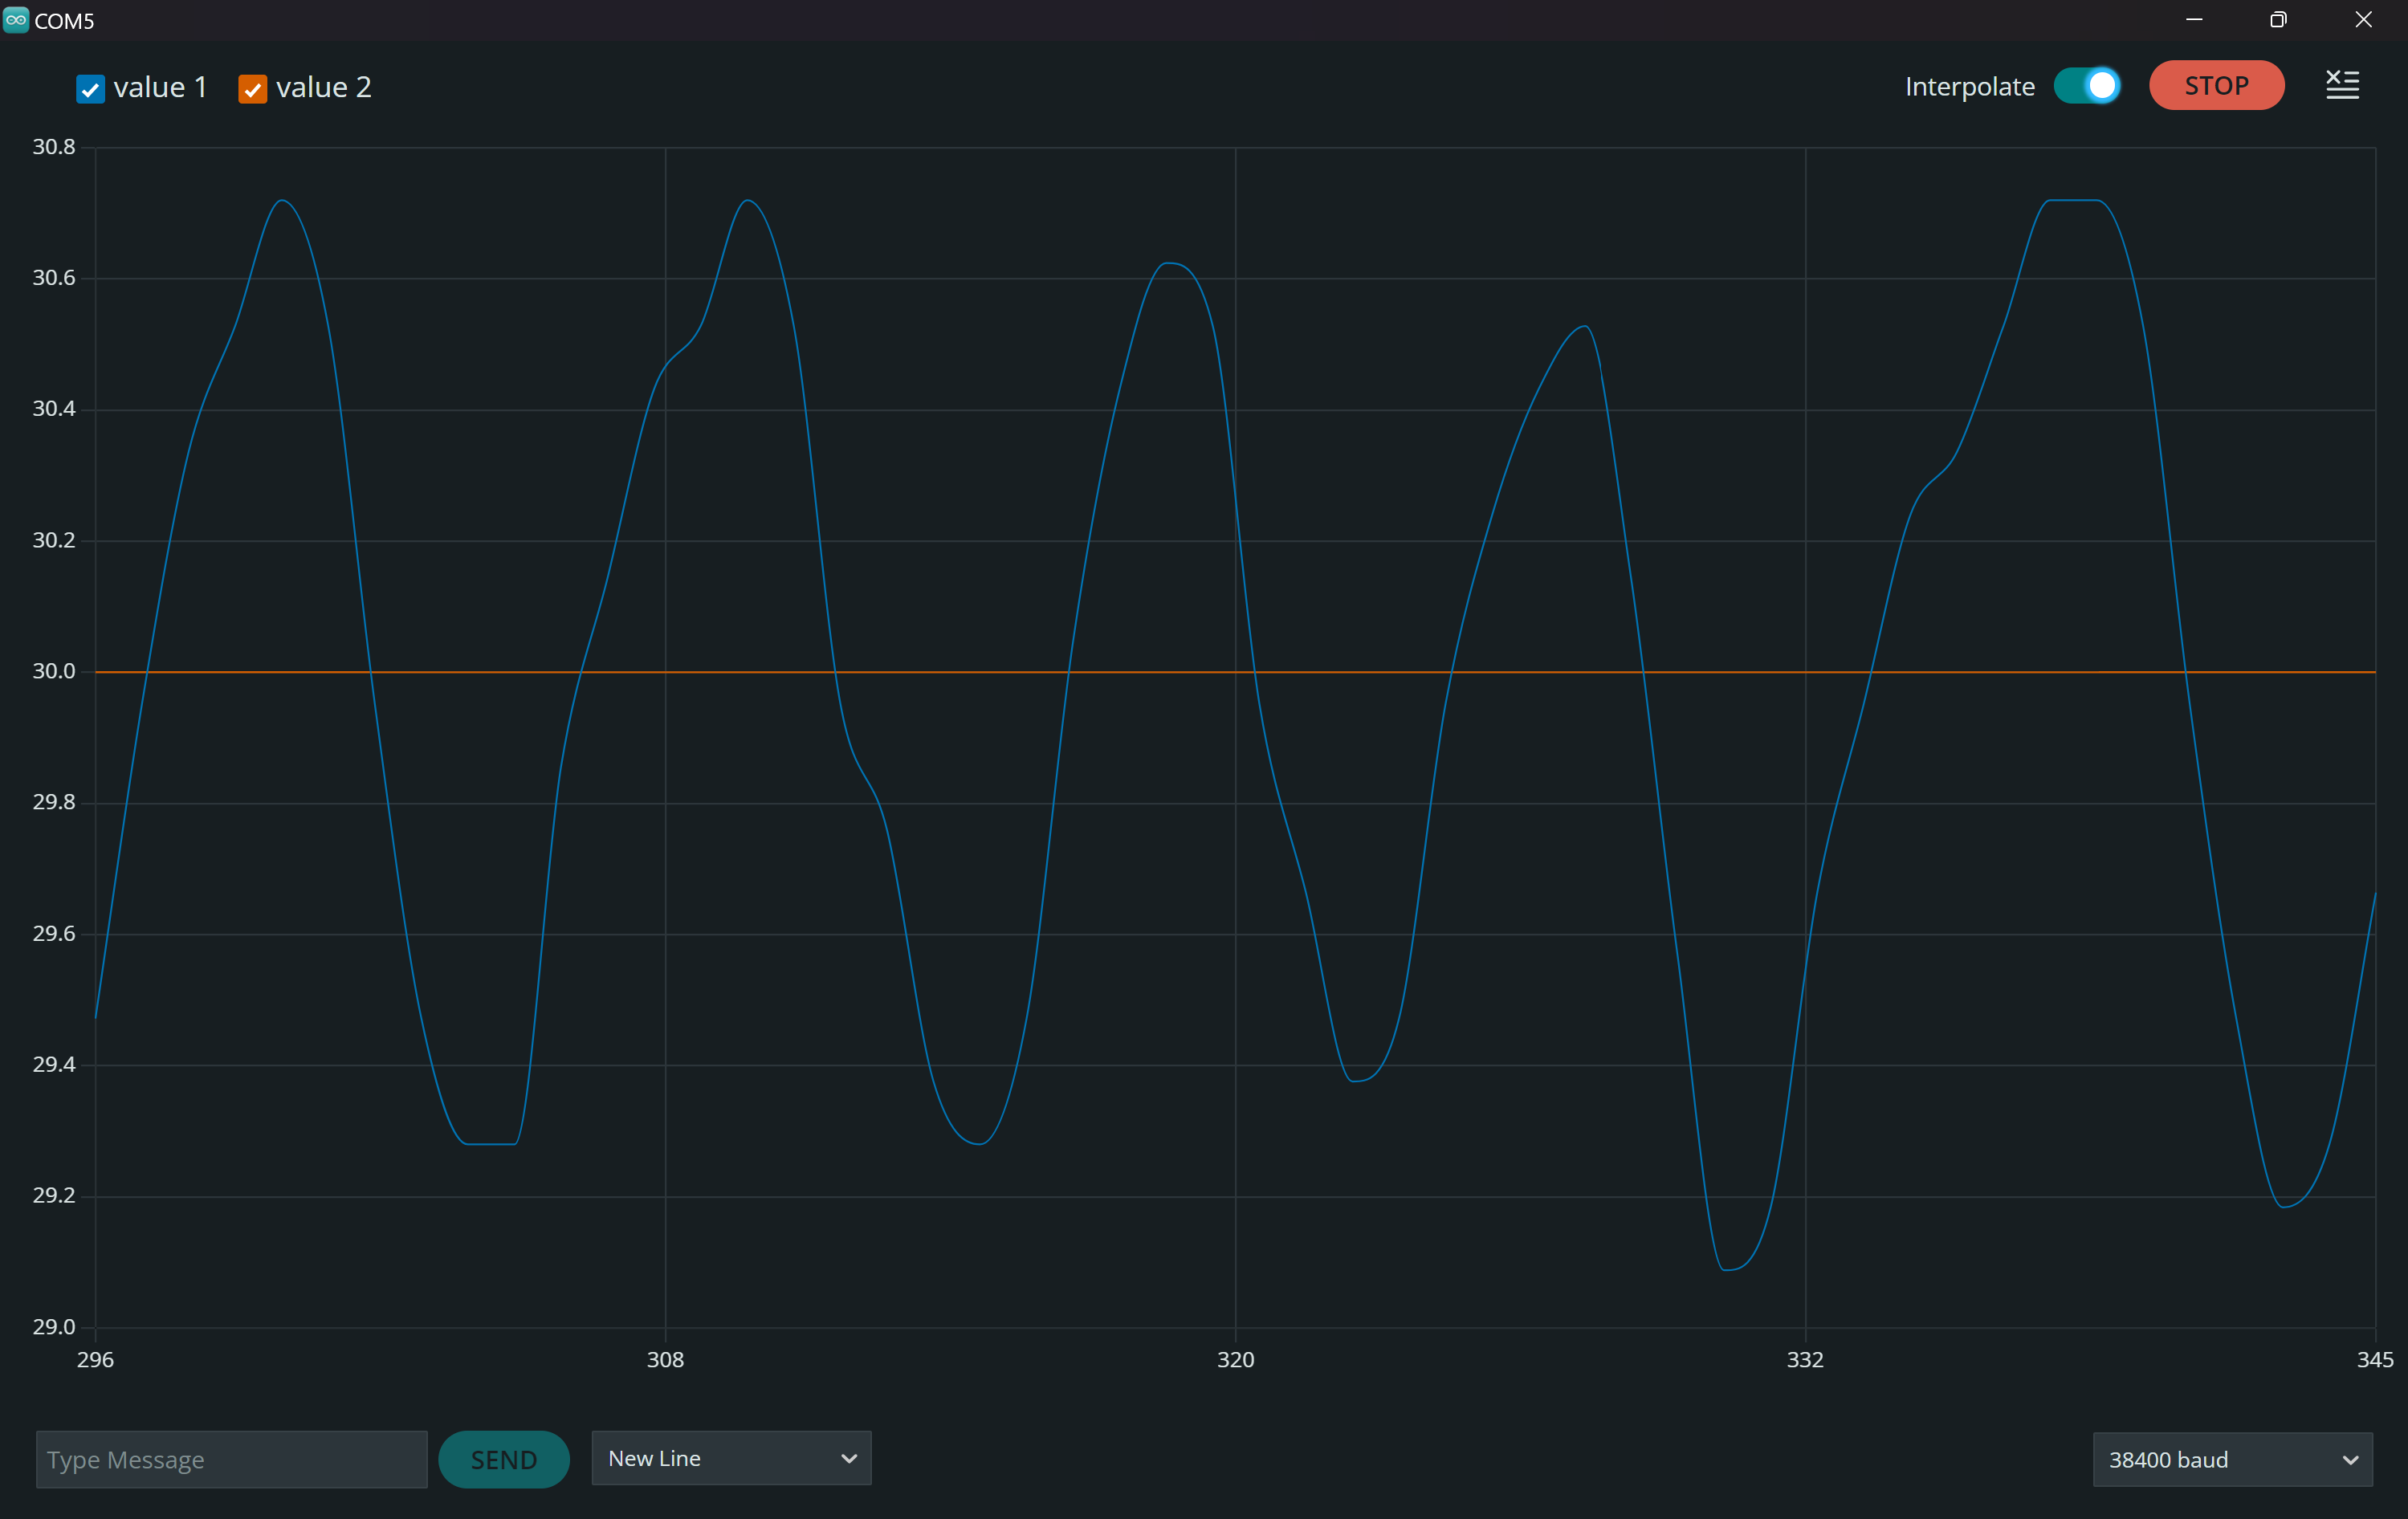
\includegraphics[width=0.95\linewidth]{images/q1/SS_10_10_0.png} 
		\caption{steady state response}
    \end{subfigure}\vspace{-1mm}
    \caption{serial plots of response for $K_P=10$, $K_I=10$, $K_D=0$}
\end{figure}
\vspace{-5mm}
\begin{figure}[h]
    \centering
    \begin{subfigure}{.44\textwidth}
        \centering
        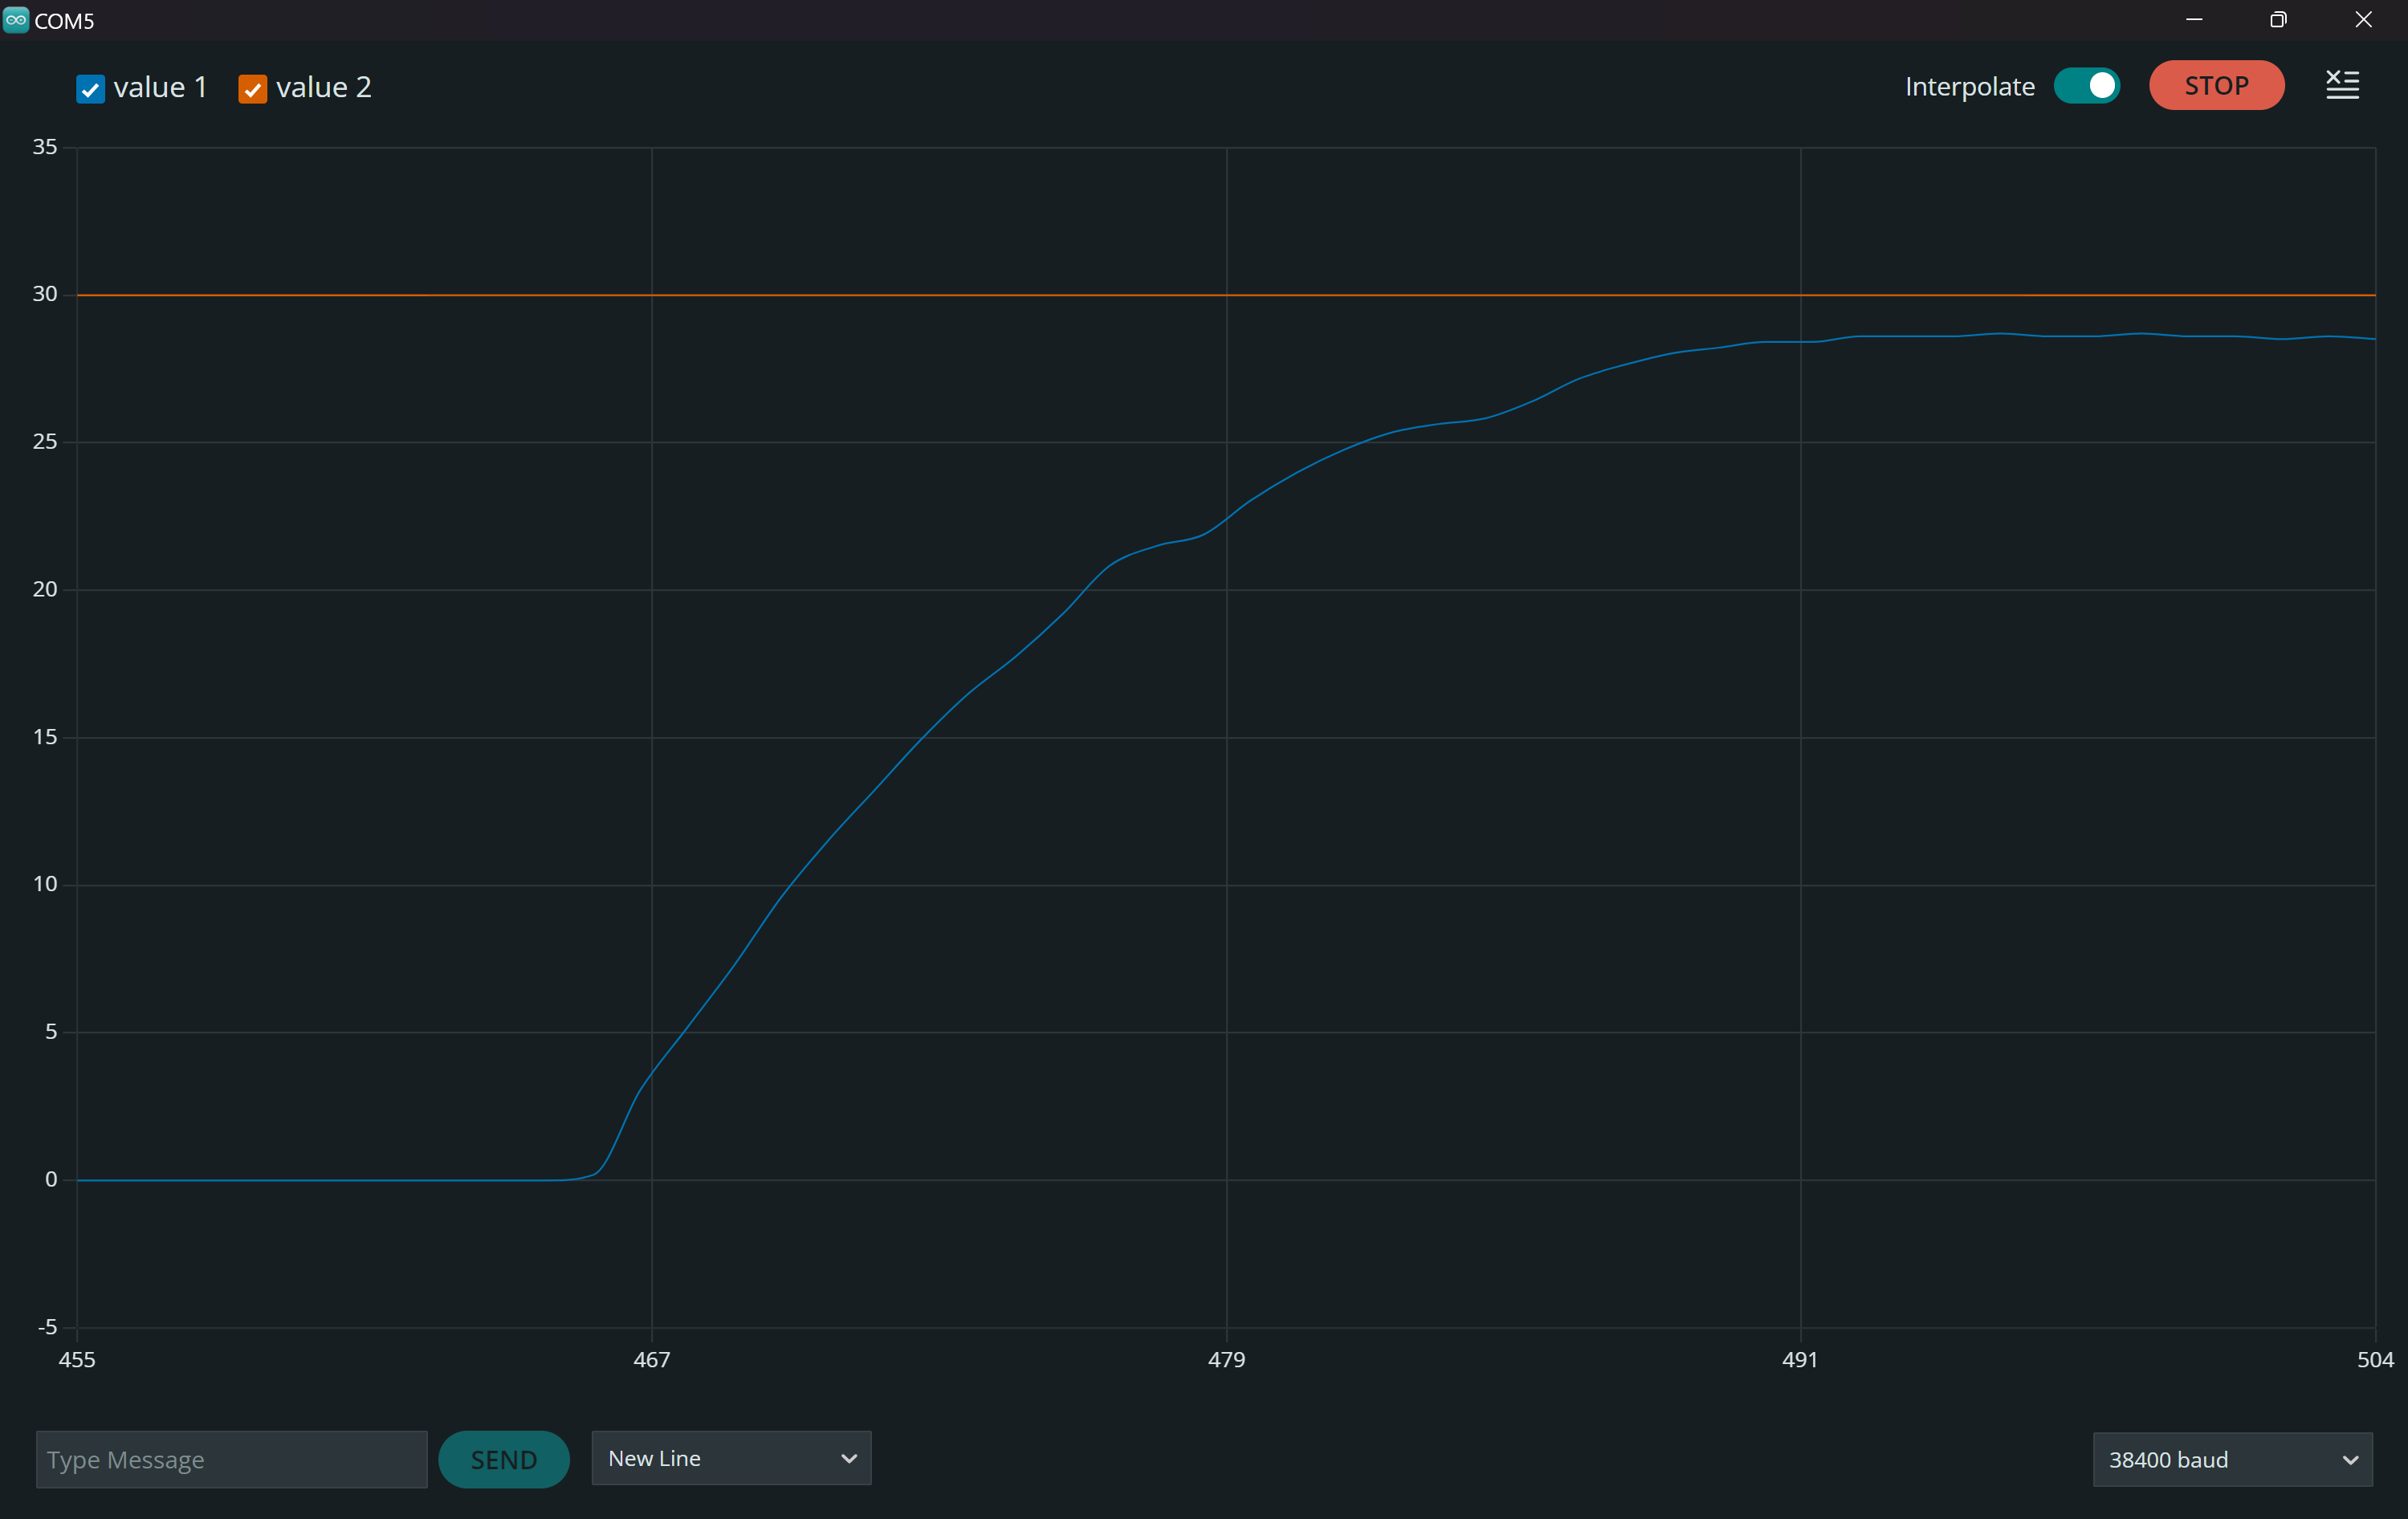
\includegraphics[width=0.95\linewidth]{images/q1/Transient_20_10_0.png}
		\caption{transient response}
    \end{subfigure}
    \begin{subfigure}{.44\textwidth}
        \centering
        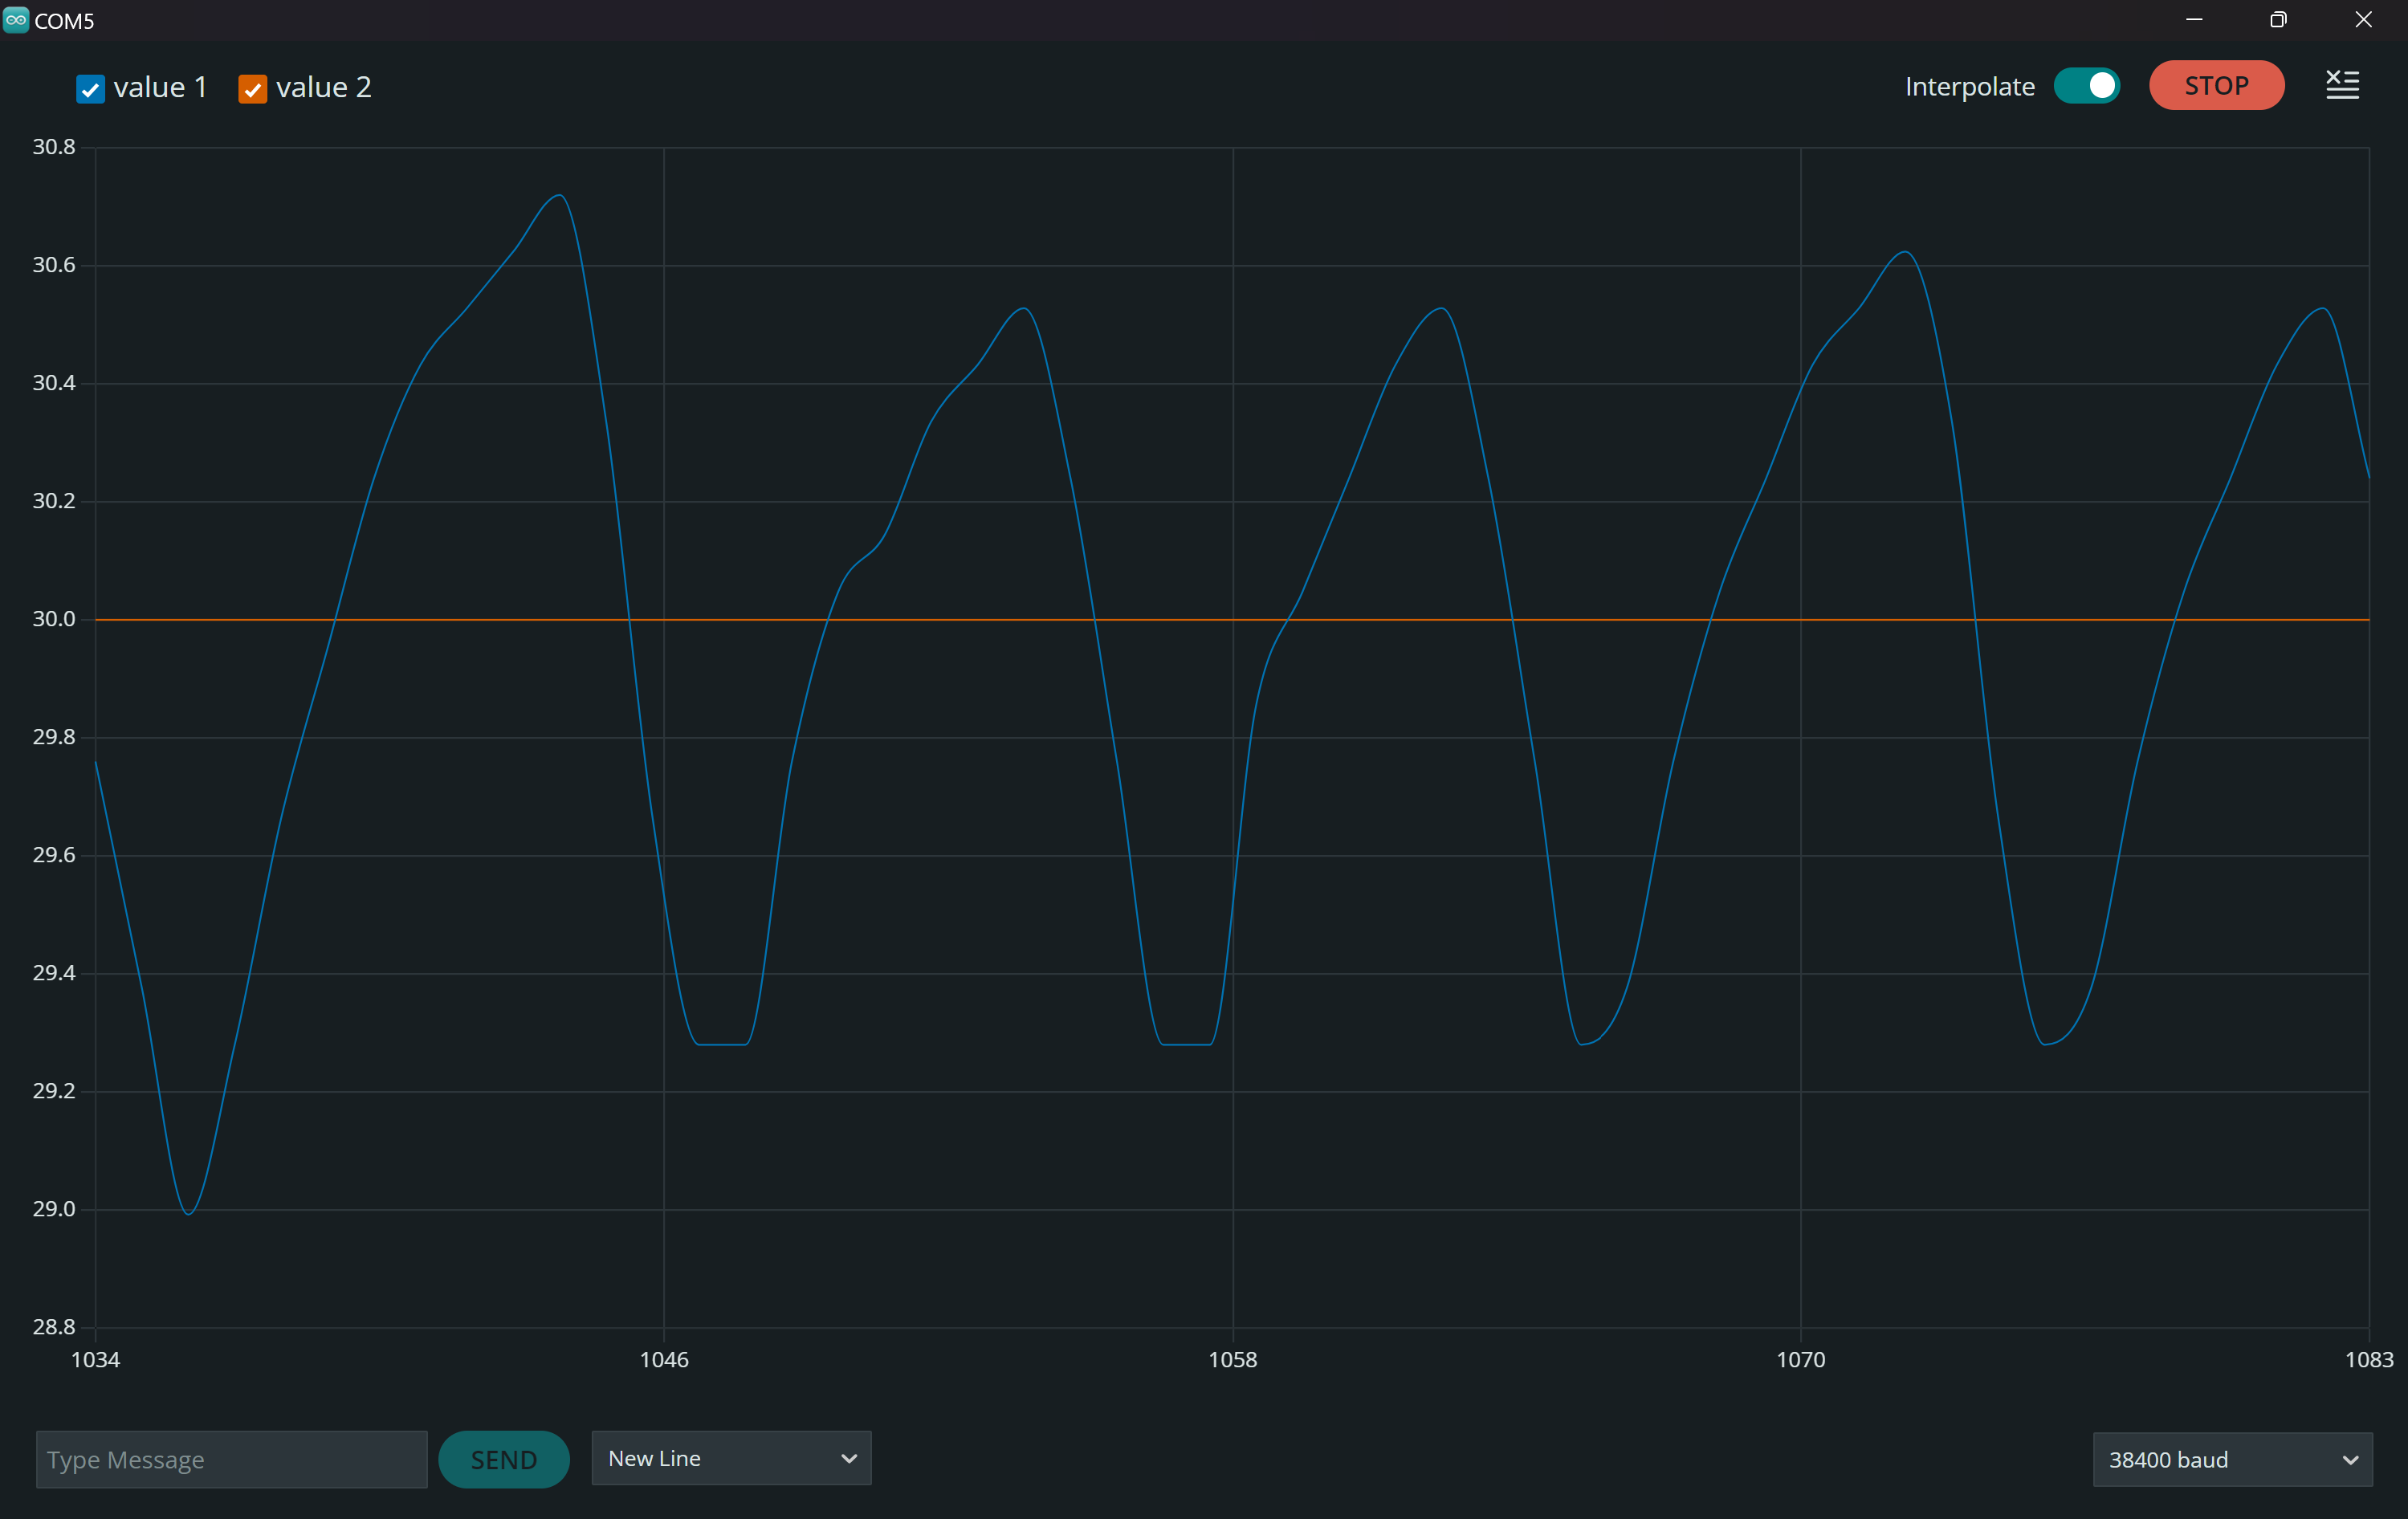
\includegraphics[width=0.95\linewidth]{images/q1/SS_20_10_0.png} 
		\caption{steady state response}
    \end{subfigure}\vspace{-1mm}
    \caption{serial plots of response for $K_P=20$, $K_I=10$, $K_D=0$}
\end{figure}
\vspace{-5mm}
\begin{figure}[h]
    \centering
    \begin{subfigure}{.44\textwidth}
        \centering
        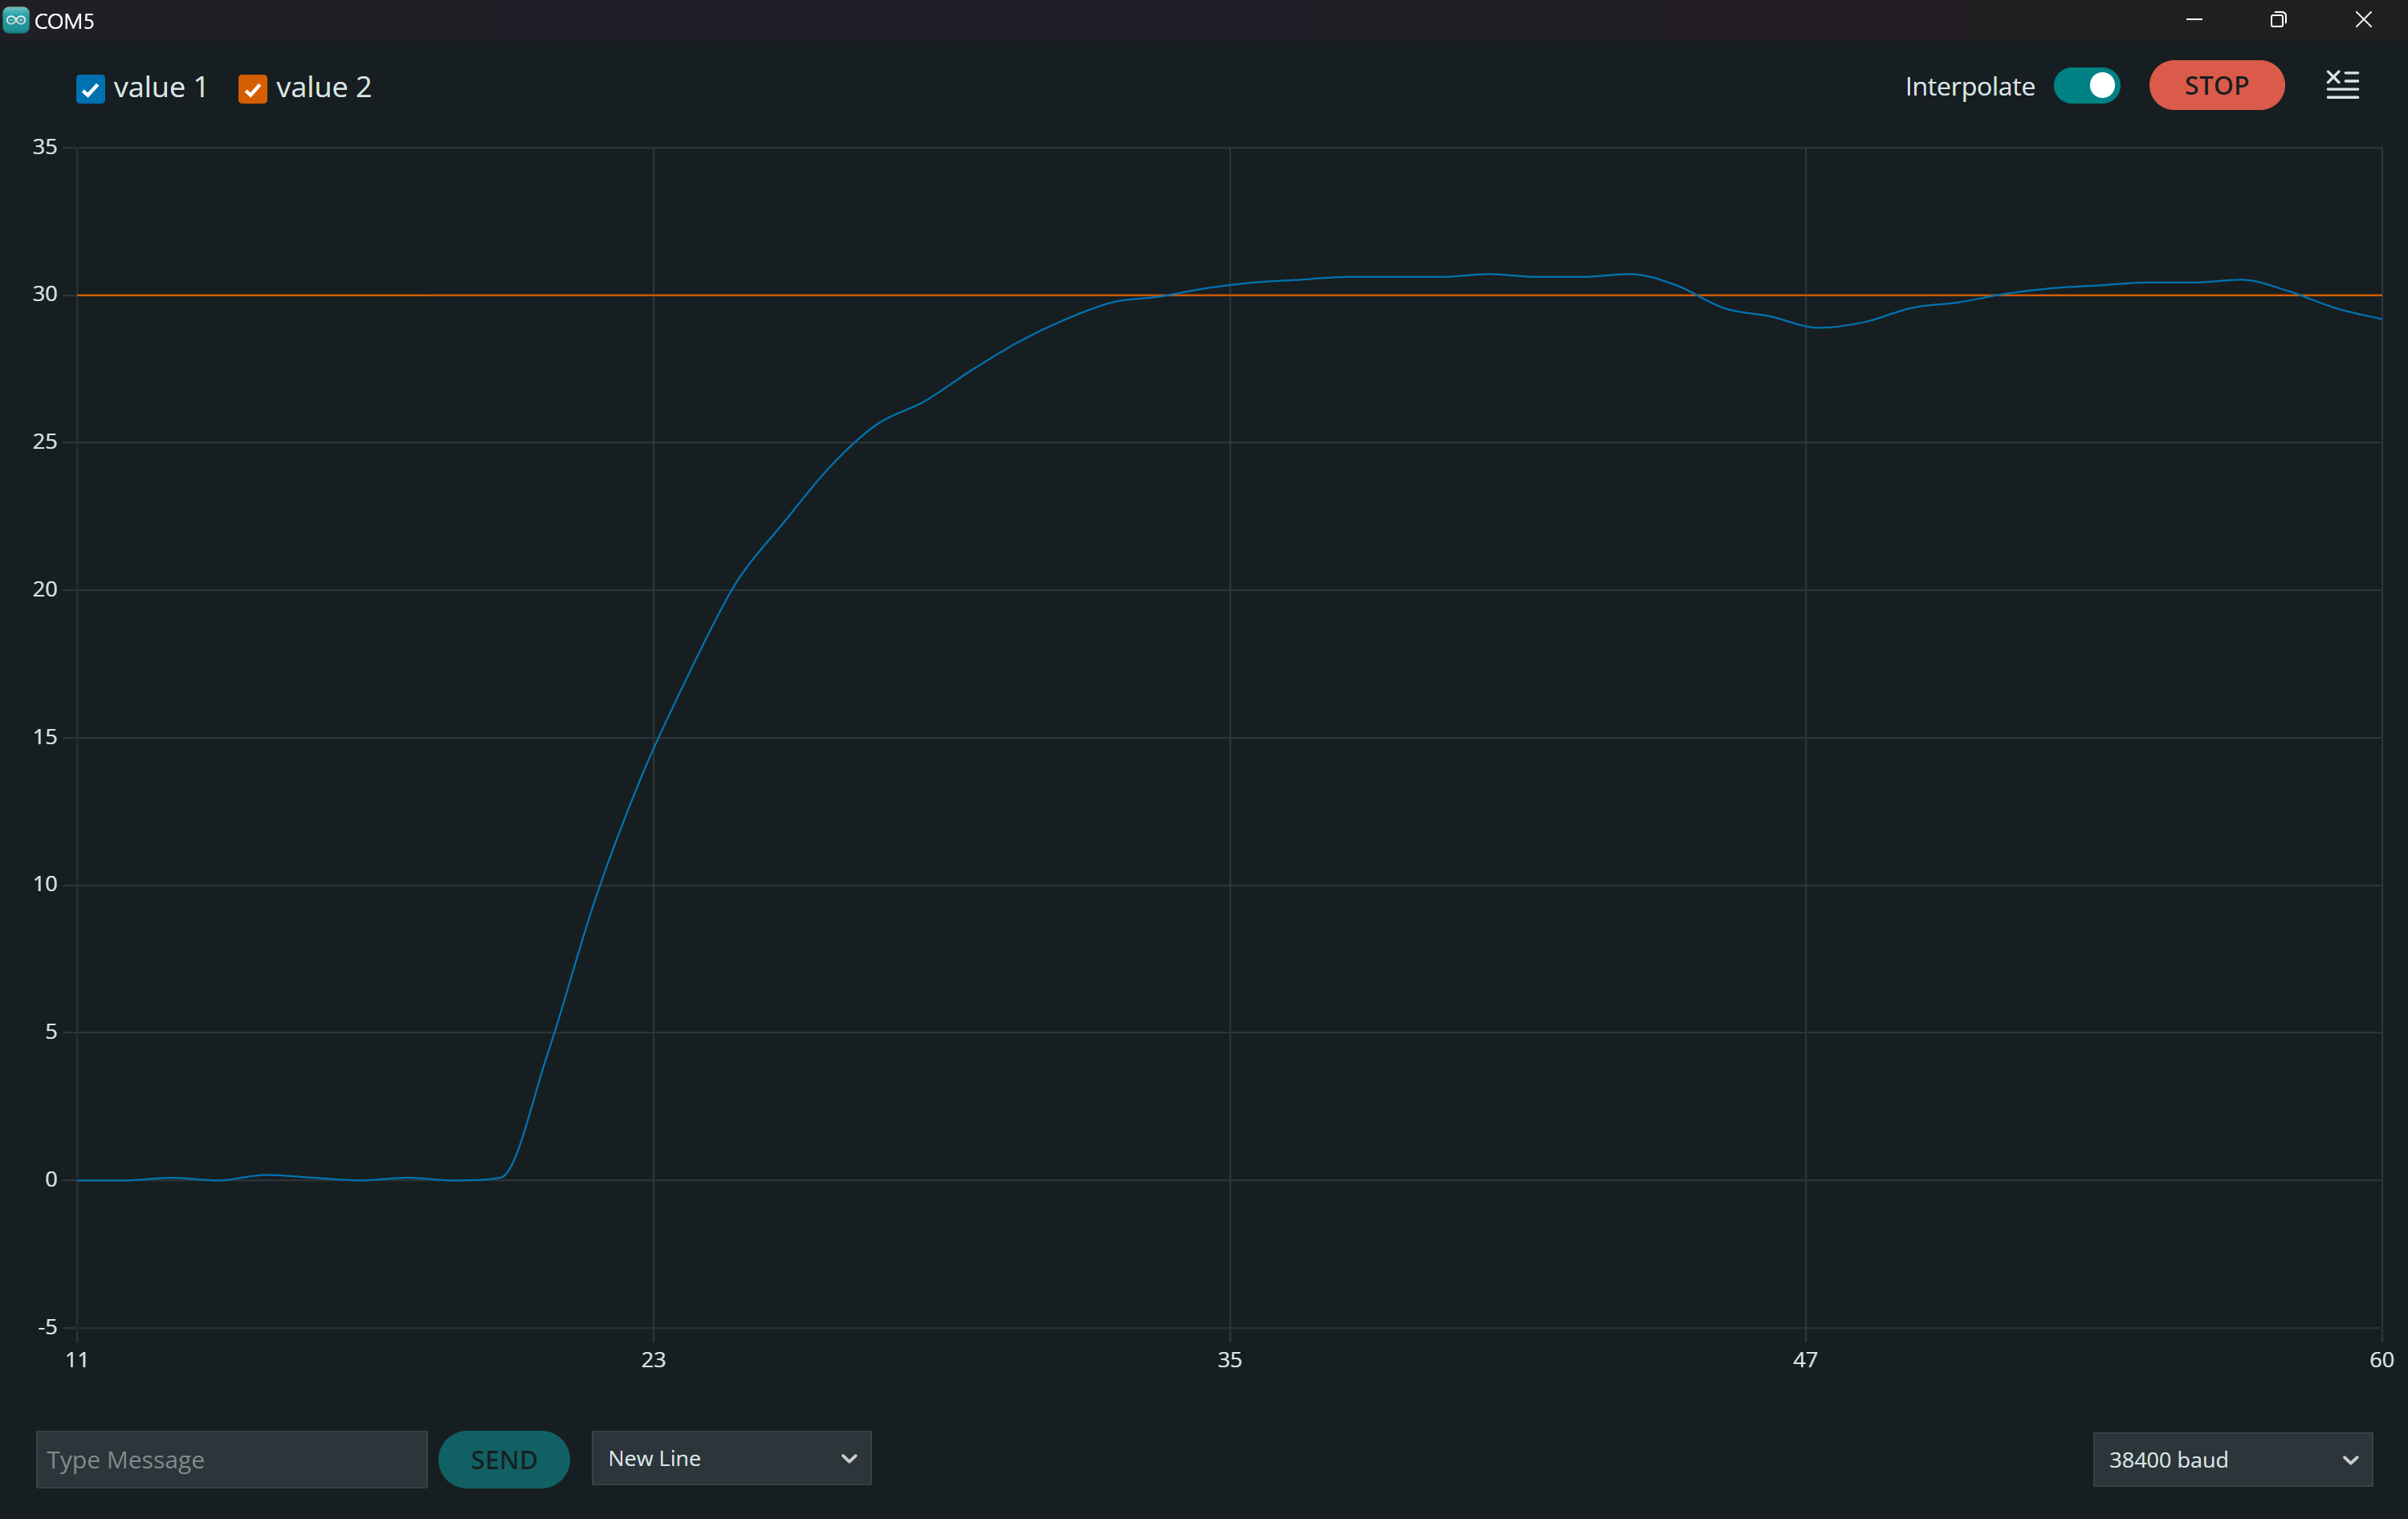
\includegraphics[width=0.95\linewidth]{images/q1/Transient_30_10_0.png}
		\caption{transient response}
    \end{subfigure}
    \begin{subfigure}{.44\textwidth}
        \centering
        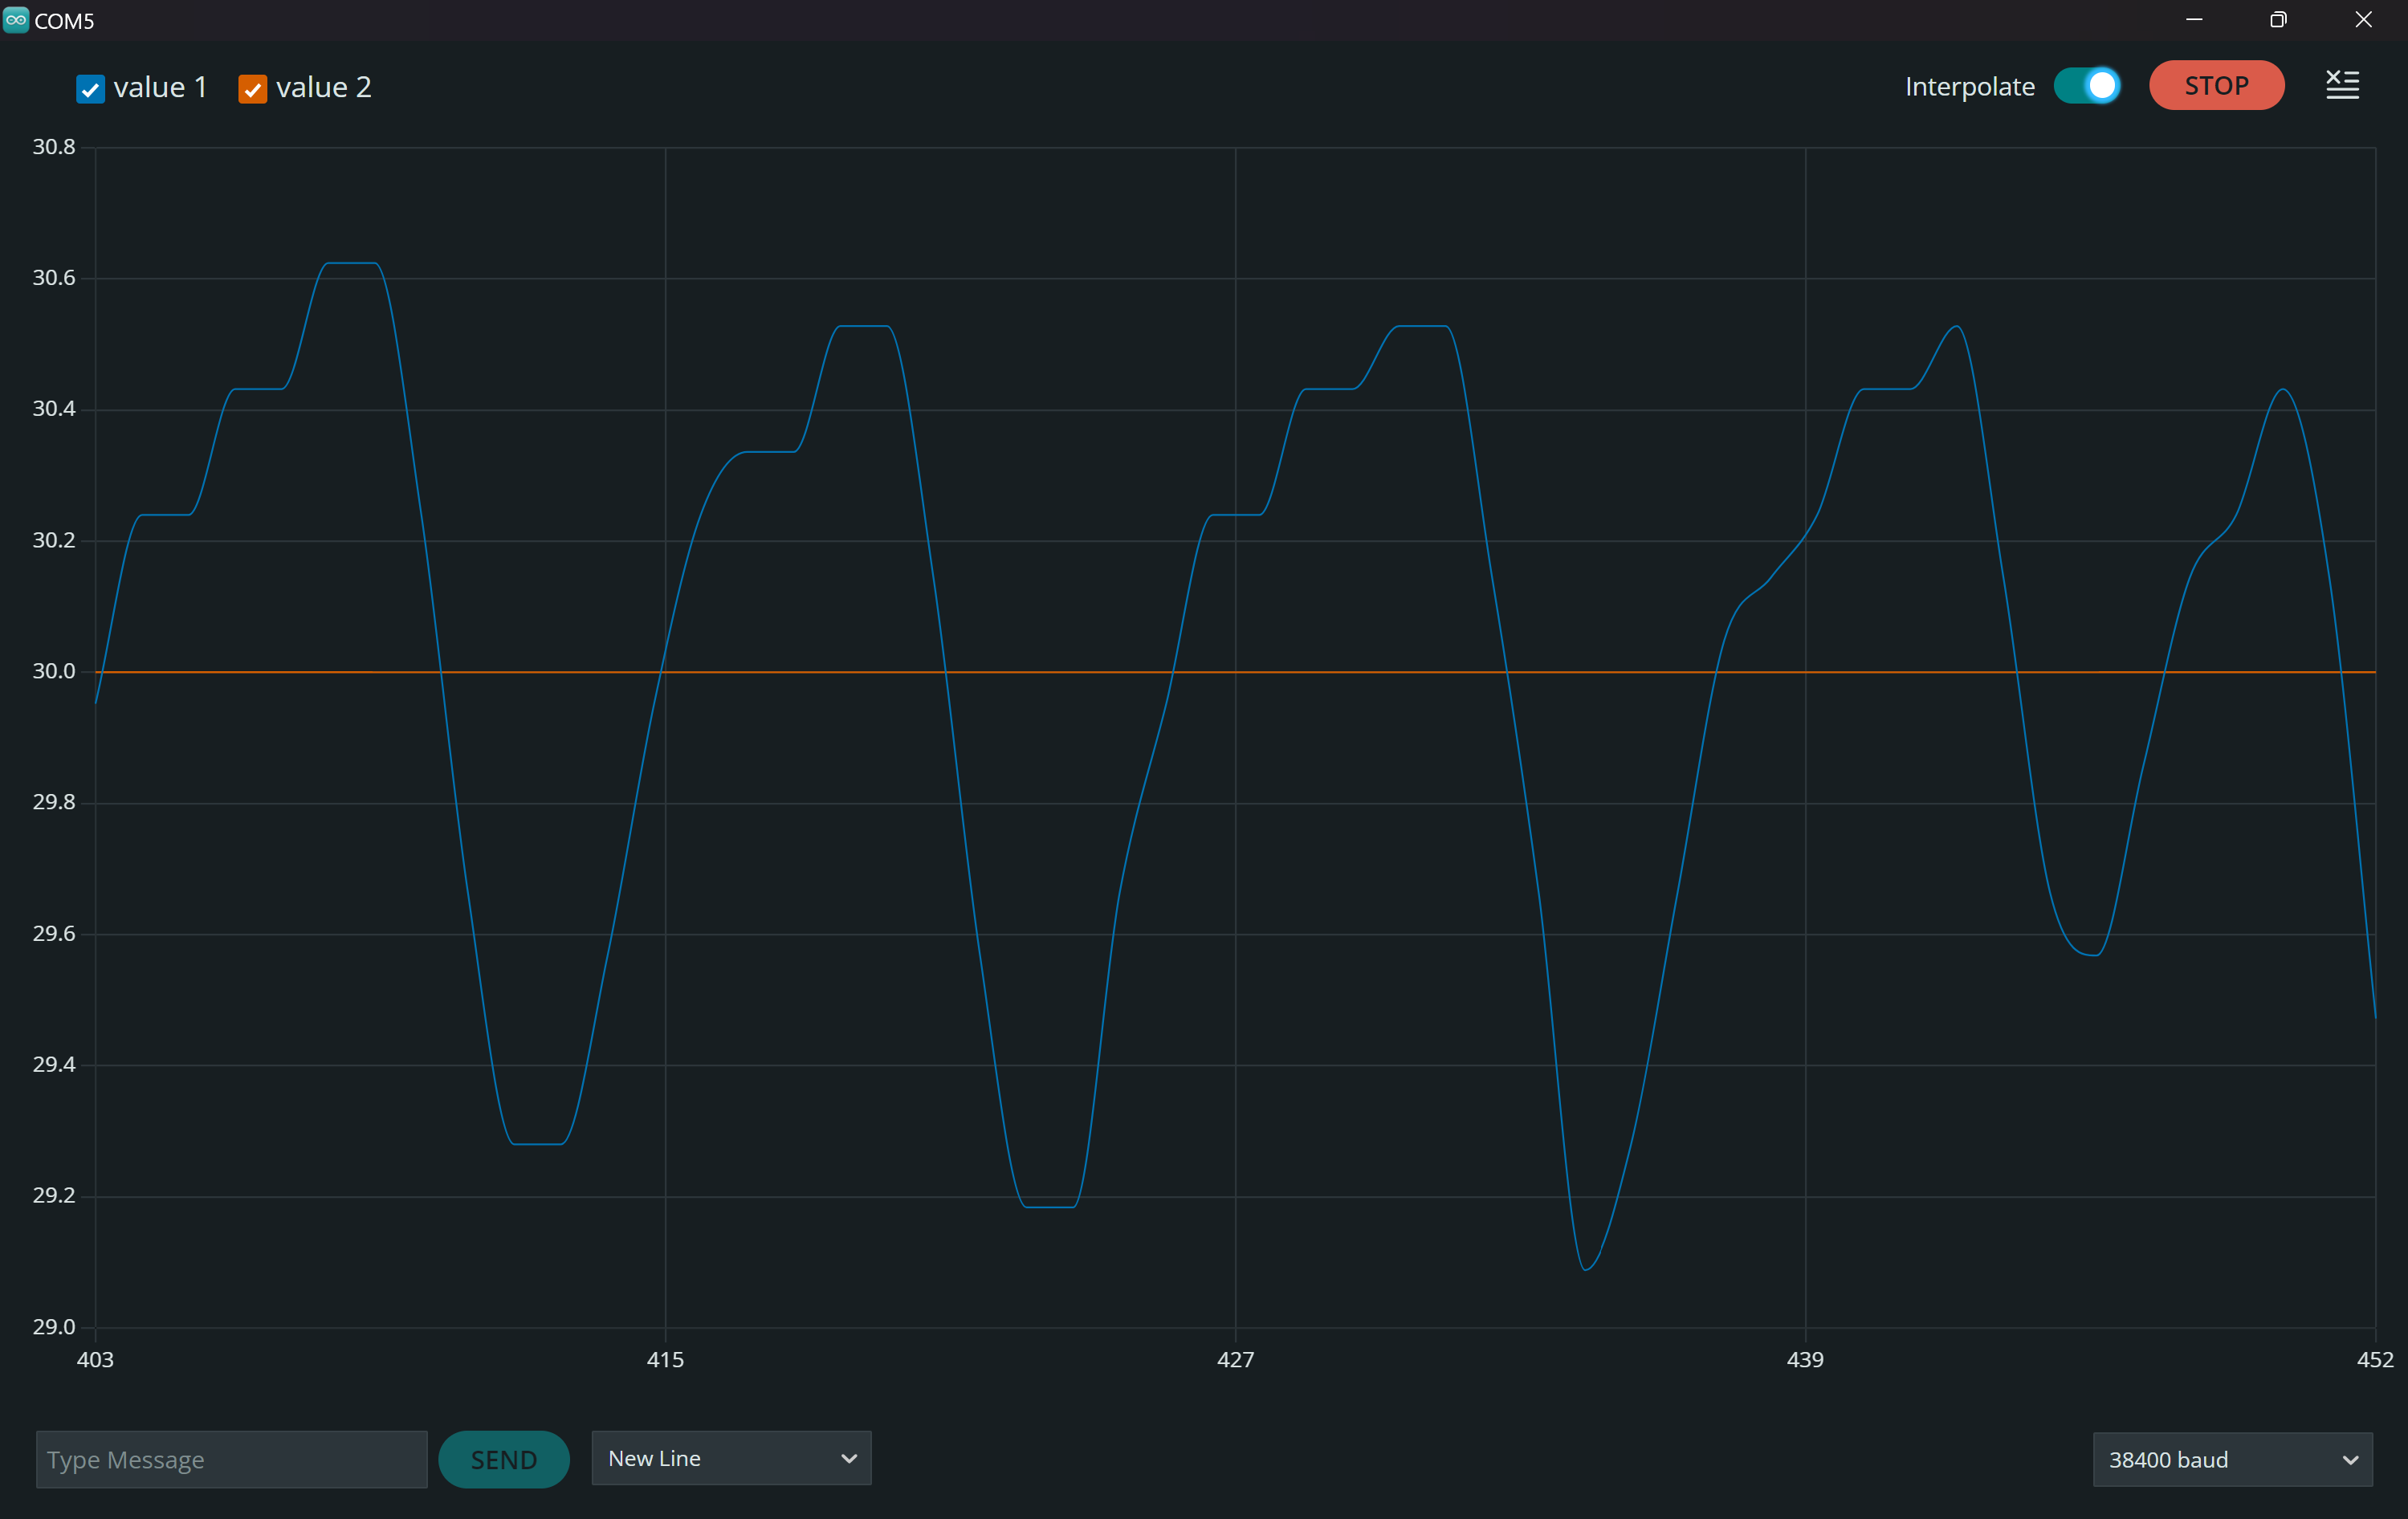
\includegraphics[width=0.95\linewidth]{images/q1/SS_30_10_0.png} 
		\caption{steady state response}
    \end{subfigure}\vspace{-1mm}
    \caption{serial plots of response for $K_P=30$, $K_I=10$, $K_D=0$}
\end{figure}

We can observe that increasing the $K_P$ term greatly improves the transient response while also maintaining a good steady state response, that is, low steady state error for a shorter settling time.

\pagebreak

\subsubsection{Varying $K_I$}

\begin{figure}[h]
    \centering
    % \begin{subfigure}{.49\textwidth}
    %     \centering
    %     \includegraphics[width=0.95\linewidth]{images/q1/10_10_0.png}
	% 	\caption{$K_I=10$}
    % \end{subfigure}
    \begin{subfigure}{.49\textwidth}
        \centering
        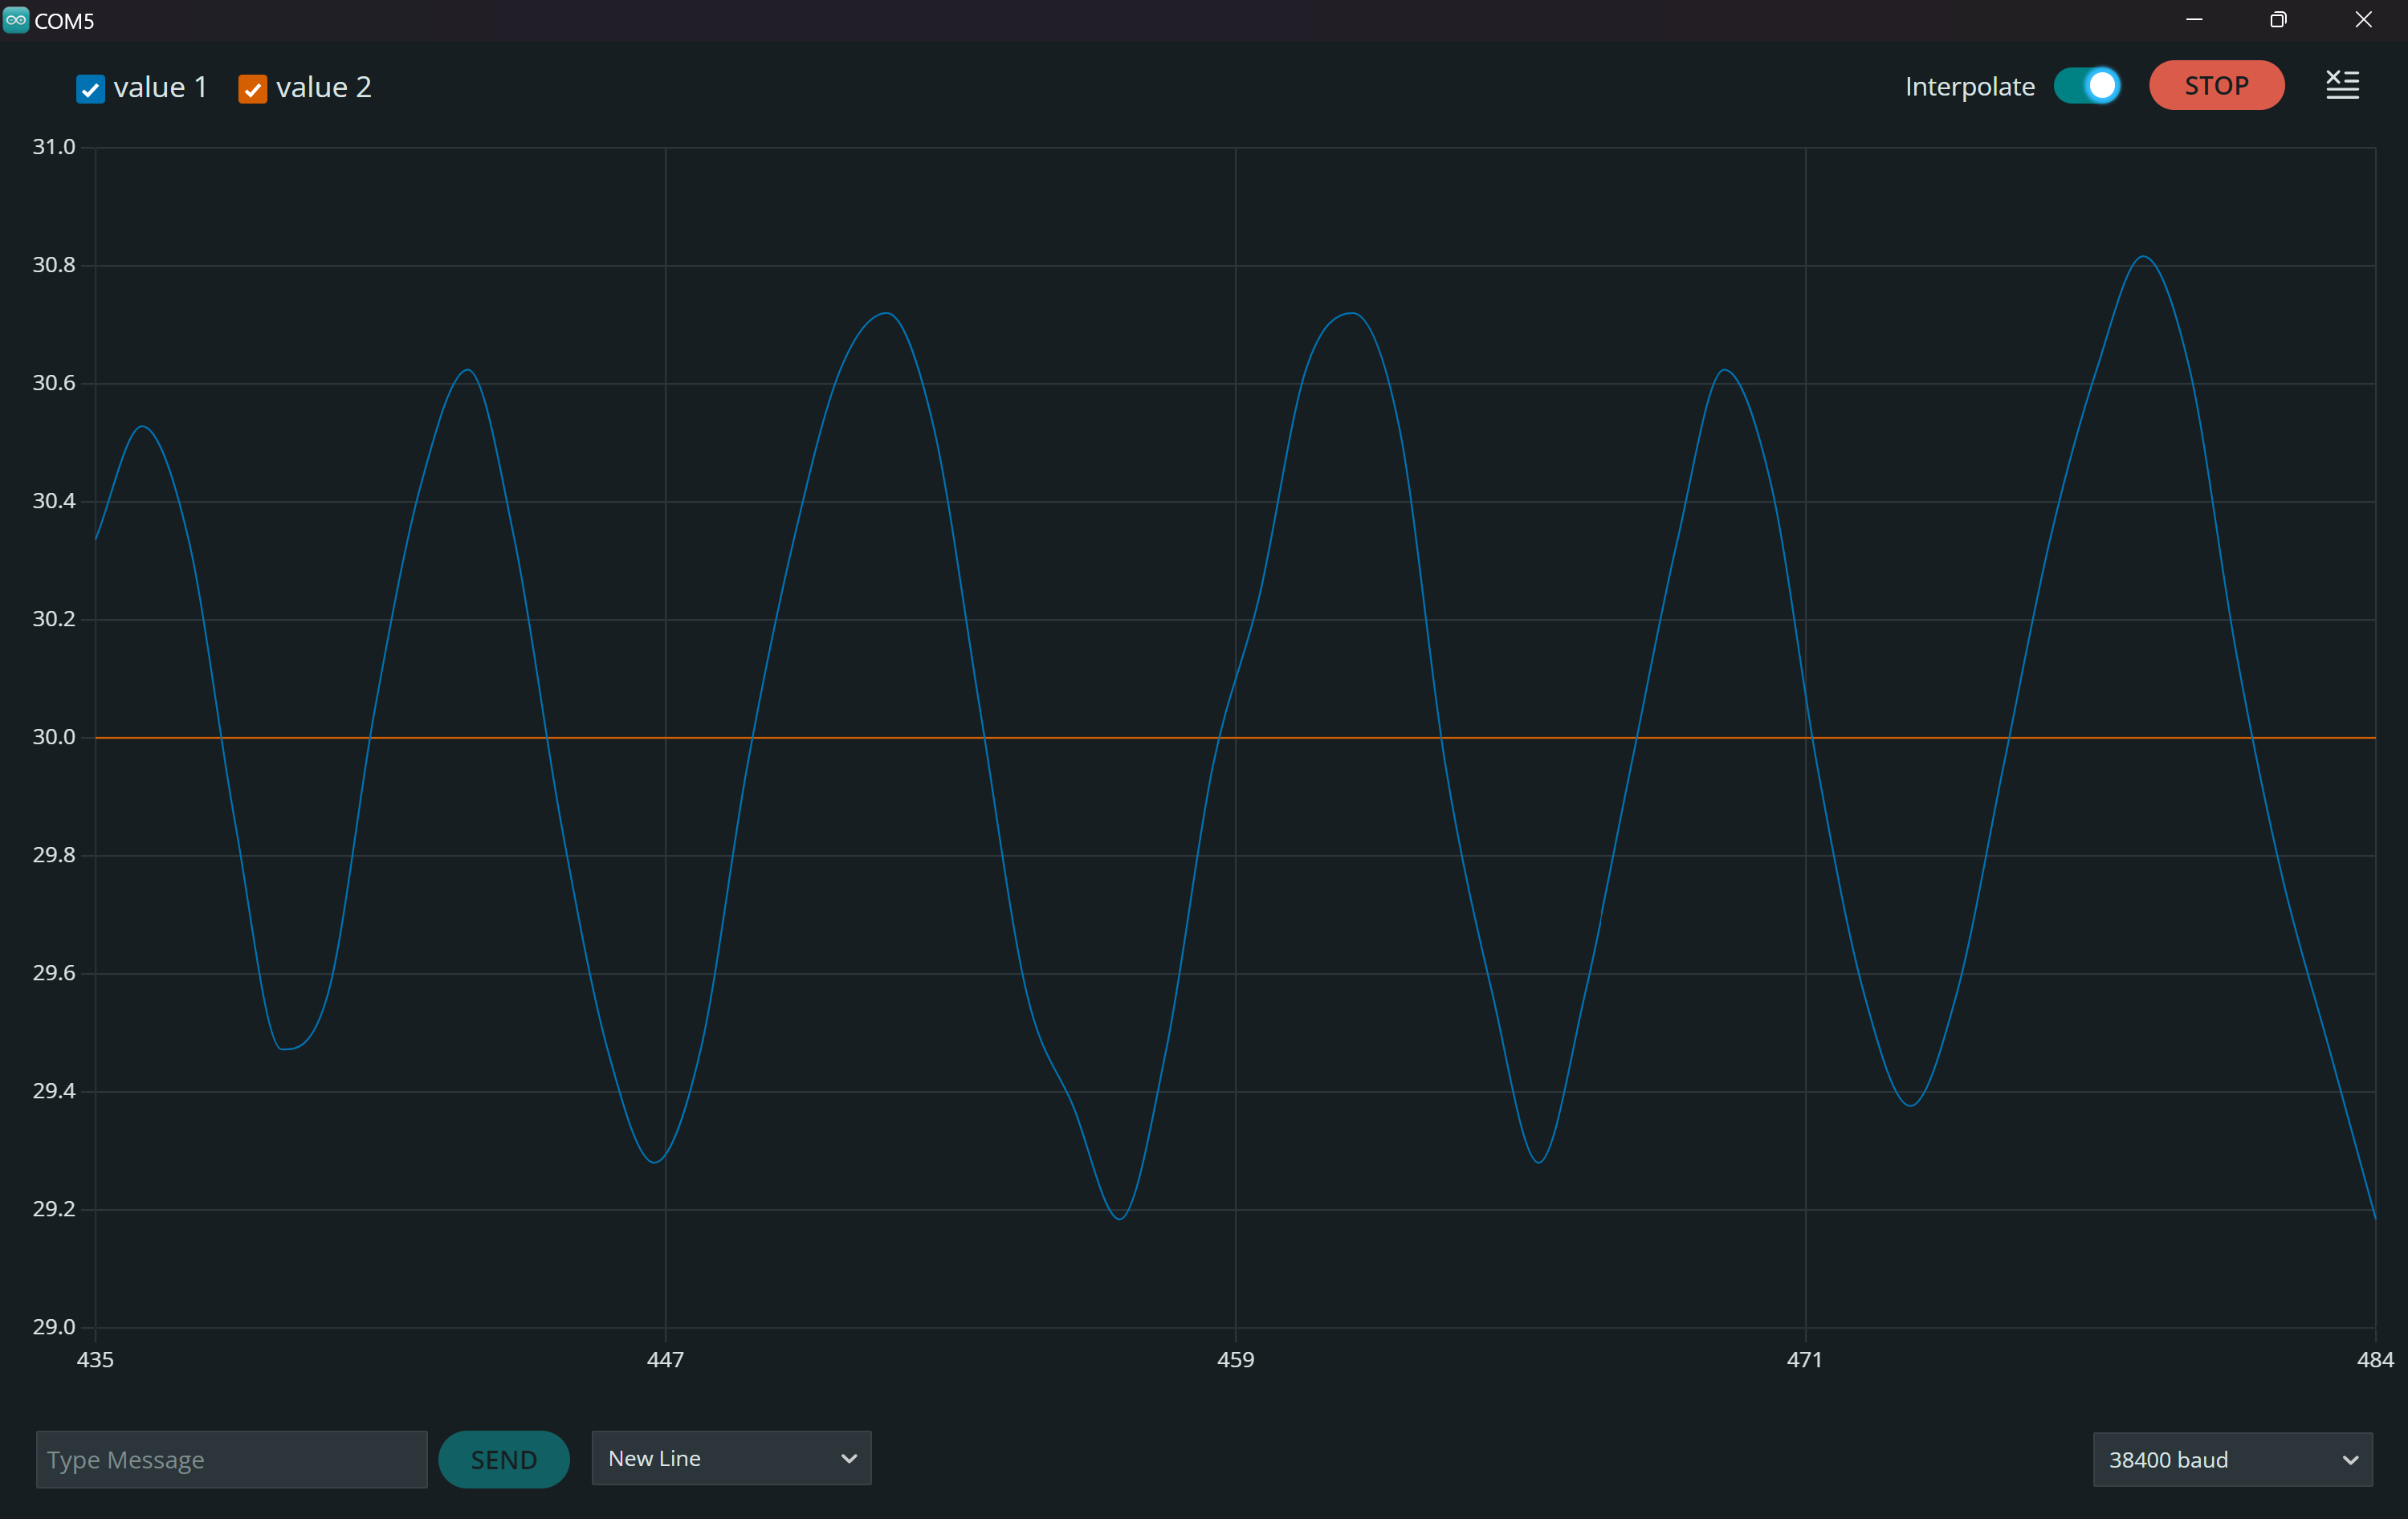
\includegraphics[width=0.95\linewidth]{images/q1/10_20_0.png} 
		\caption{$K_I=20$}
    \end{subfigure}
	\begin{subfigure}{.49\textwidth}
        \centering
        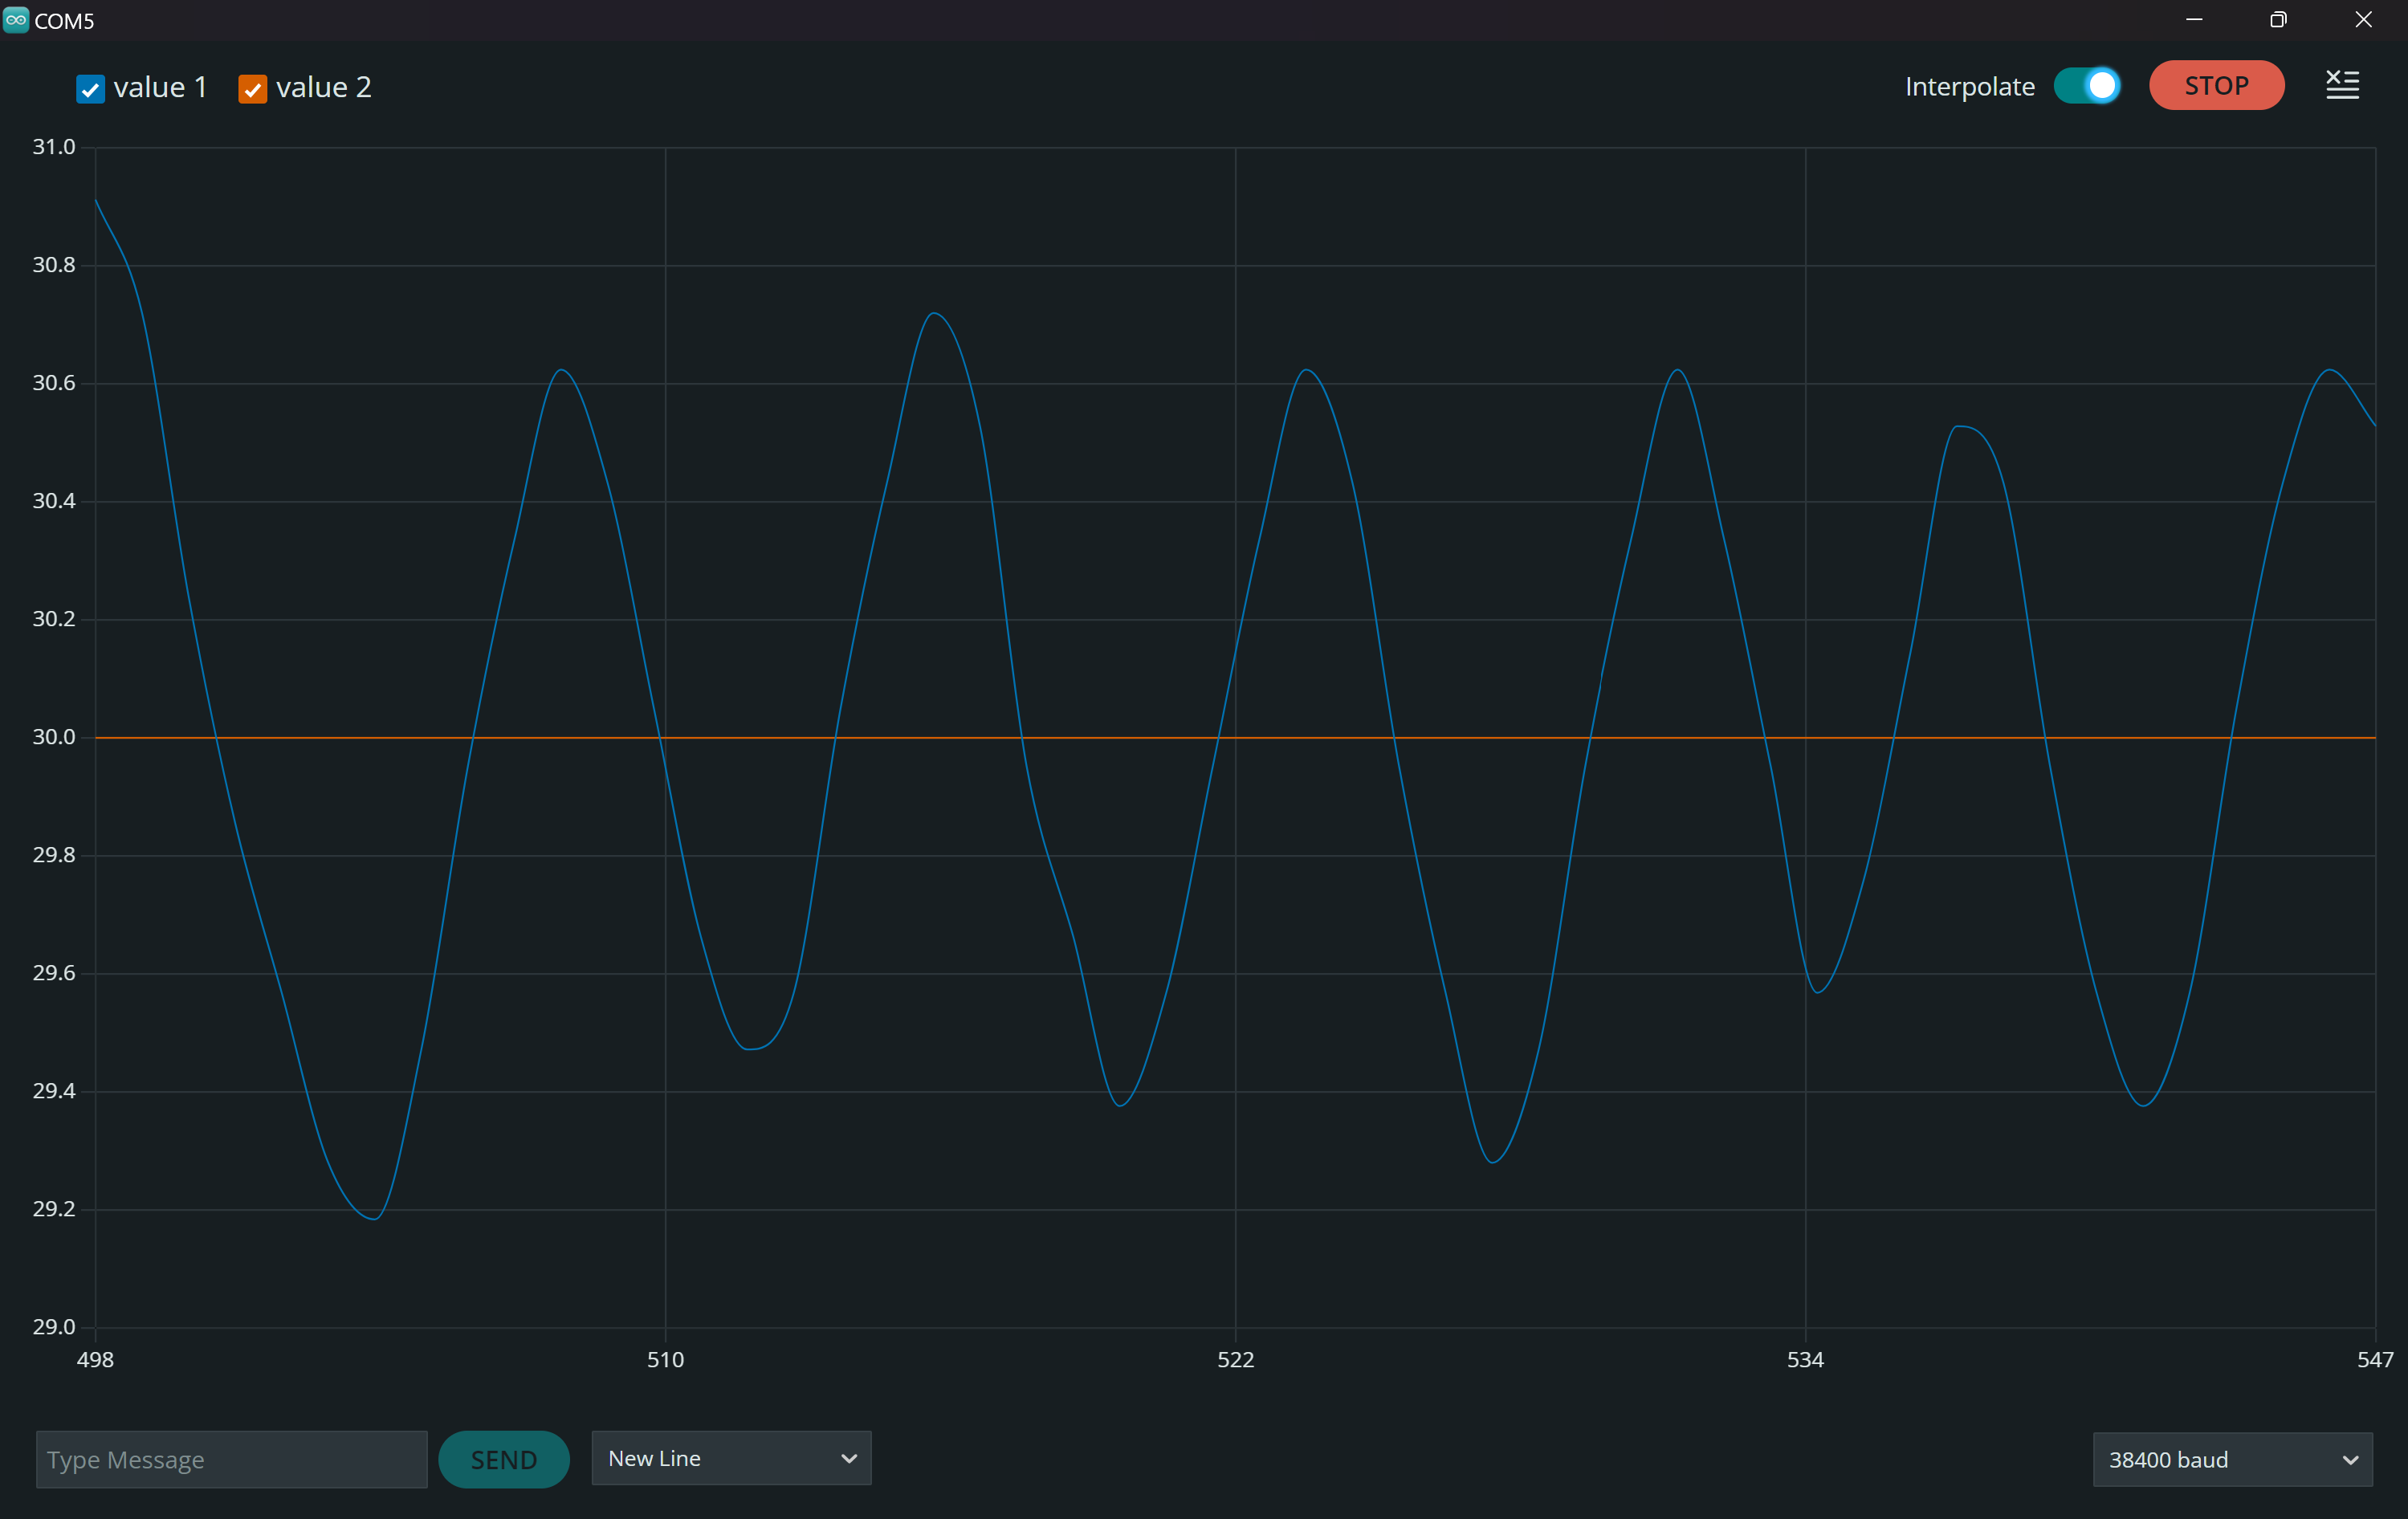
\includegraphics[width=0.95\linewidth]{images/q1/10_30_0.png}
		\caption{$K_I=30$}
    \end{subfigure}
    \begin{subfigure}{.49\textwidth}
        \centering
        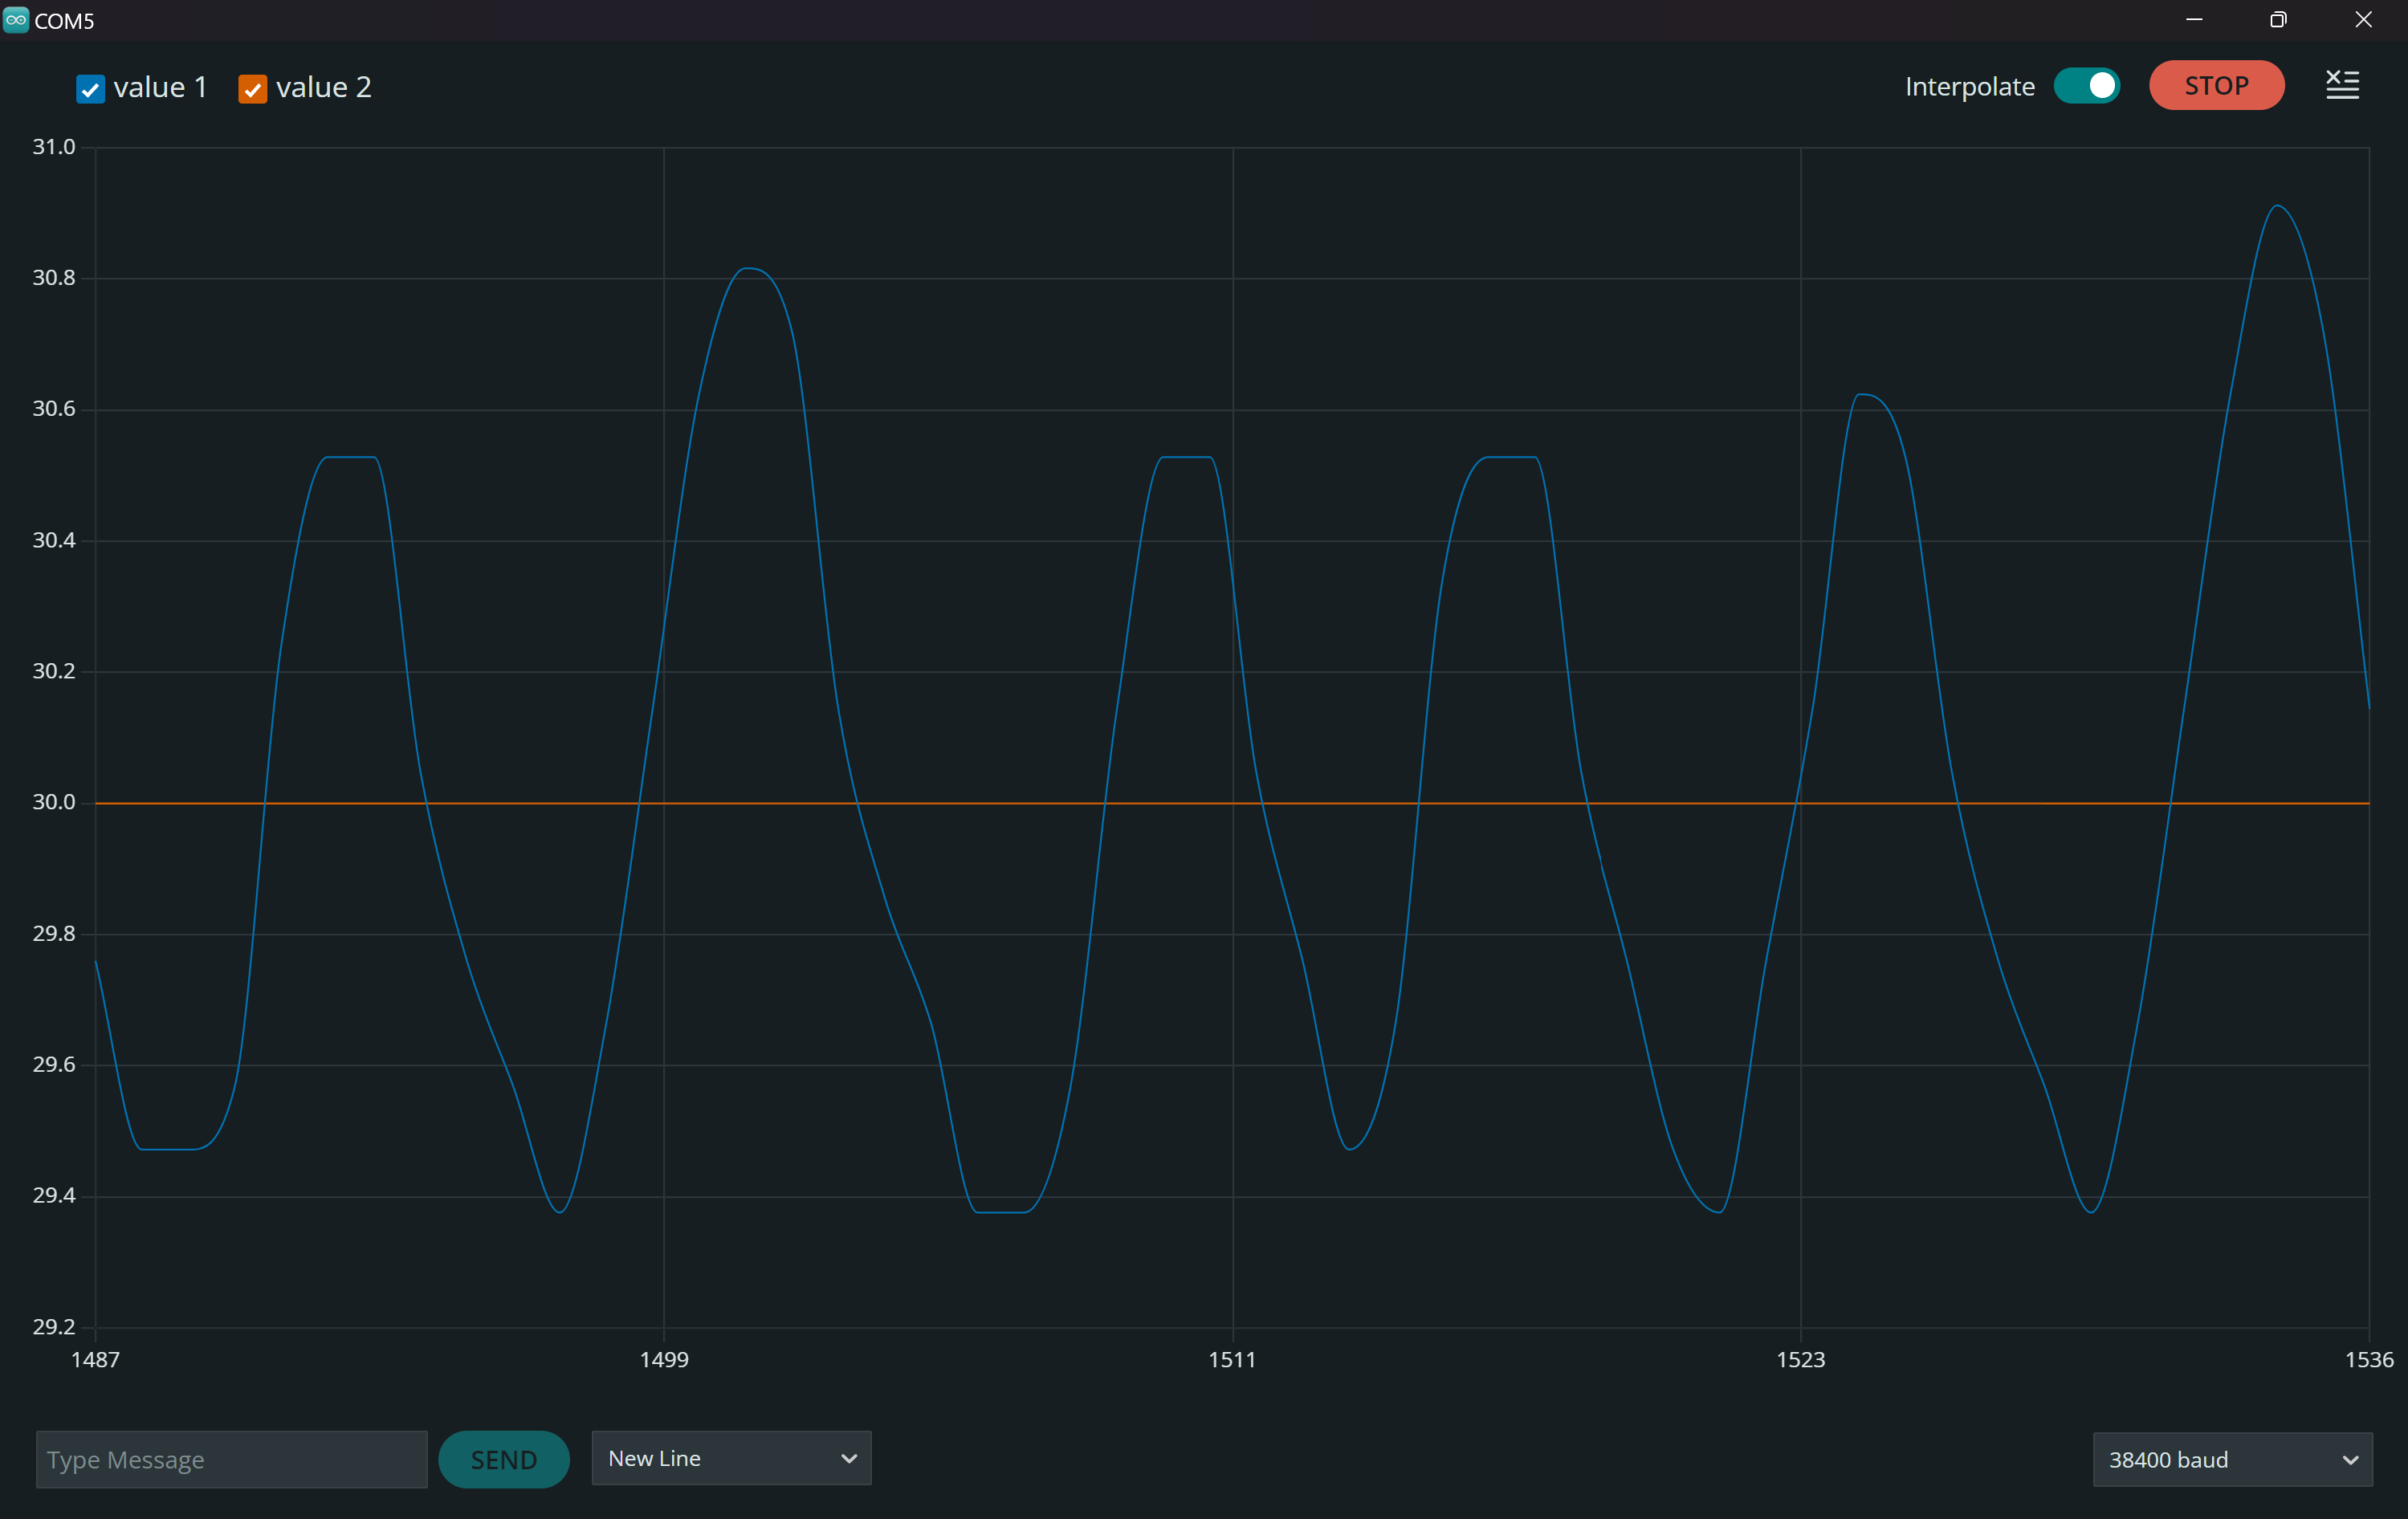
\includegraphics[width=0.95\linewidth]{images/q1/10_40_0.png} 
		\caption{$K_I=40$}
    \end{subfigure}
    \caption{transient responses for $K_P=10$, $K_D=0$ and various values of $K_I$}
\end{figure}

We can observe that increasing the $K_I$ term decreases the steady state error, but its effects diminish as we keep increasing its value indefinitely.

\subsubsection{Conclusion}
From the analysis of changing the values of PID gains, $K_P$, $K_I$ and $K_D$, we have concluded that a reasonable trade-off is required between $K_P$ and $K_I$ to get a less settling time along with negligible steady state error. The $K_D$ Kd term is detrimental to our system due to the presence of sensor noise of the encoder due to which we have decided to reduce the $K_D$ term to 0 for further analysis. After fine tuning the $K_P$ and $K_I$ values, we have reached the optimum values for these terms by hit and trial (by comparing the settling time, maximum peak overshoot and steady state error). We have found $K_P\sim40$ and $K_I\sim25$ to be the most optimum values which we will use for the further analysis.

\pagebreak

\subsection{Question 2}
What is the effect of changing the setpoint while keeping the PID gains constant?

Using $K_P = 40$, $K_I = 25$ and $K_D=0$

\begin{table}[h]
    \centering
    \begin{tabular}{|c|c|c|c|}
        \hline
        \textbf{Setpoint RPM} & \textbf{Steady State RPM} & \textbf{Steady State Error} & \textbf{Settling Time (s)} \\
        \hline\hline
        25   & 24.86 & 0.14 & 2.0  \\
        \hline
        40   & 39.89 & 0.11 & 2.2  \\
        \hline
        50   & 50.07 & 0.07 & 1.4  \\
        \hline
        60   & 59.90 & 0.10 & 1.5  \\
        \hline
        75   & 74.76 & 0.24 & 2.3  \\
        \hline
        100  & 99.84 & 0.16 & 10.1 \\
        \hline
        120  & 113.04 & 6.96 & 14.9 \\
        \hline
    \end{tabular}
    \label{tab:steady_state_metrics}
\end{table}

\subsection{Question 3}
What happens when you change the setpoint when the motor is running?

The commanded duty cycle initially shoots up suddenly regardless of the change in commanded RPMS but settles to the final commanded value if within actuator limits. For an example:

\begin{figure}[h]
    \centering
	\begin{subfigure}{.48\textwidth}
        \centering
        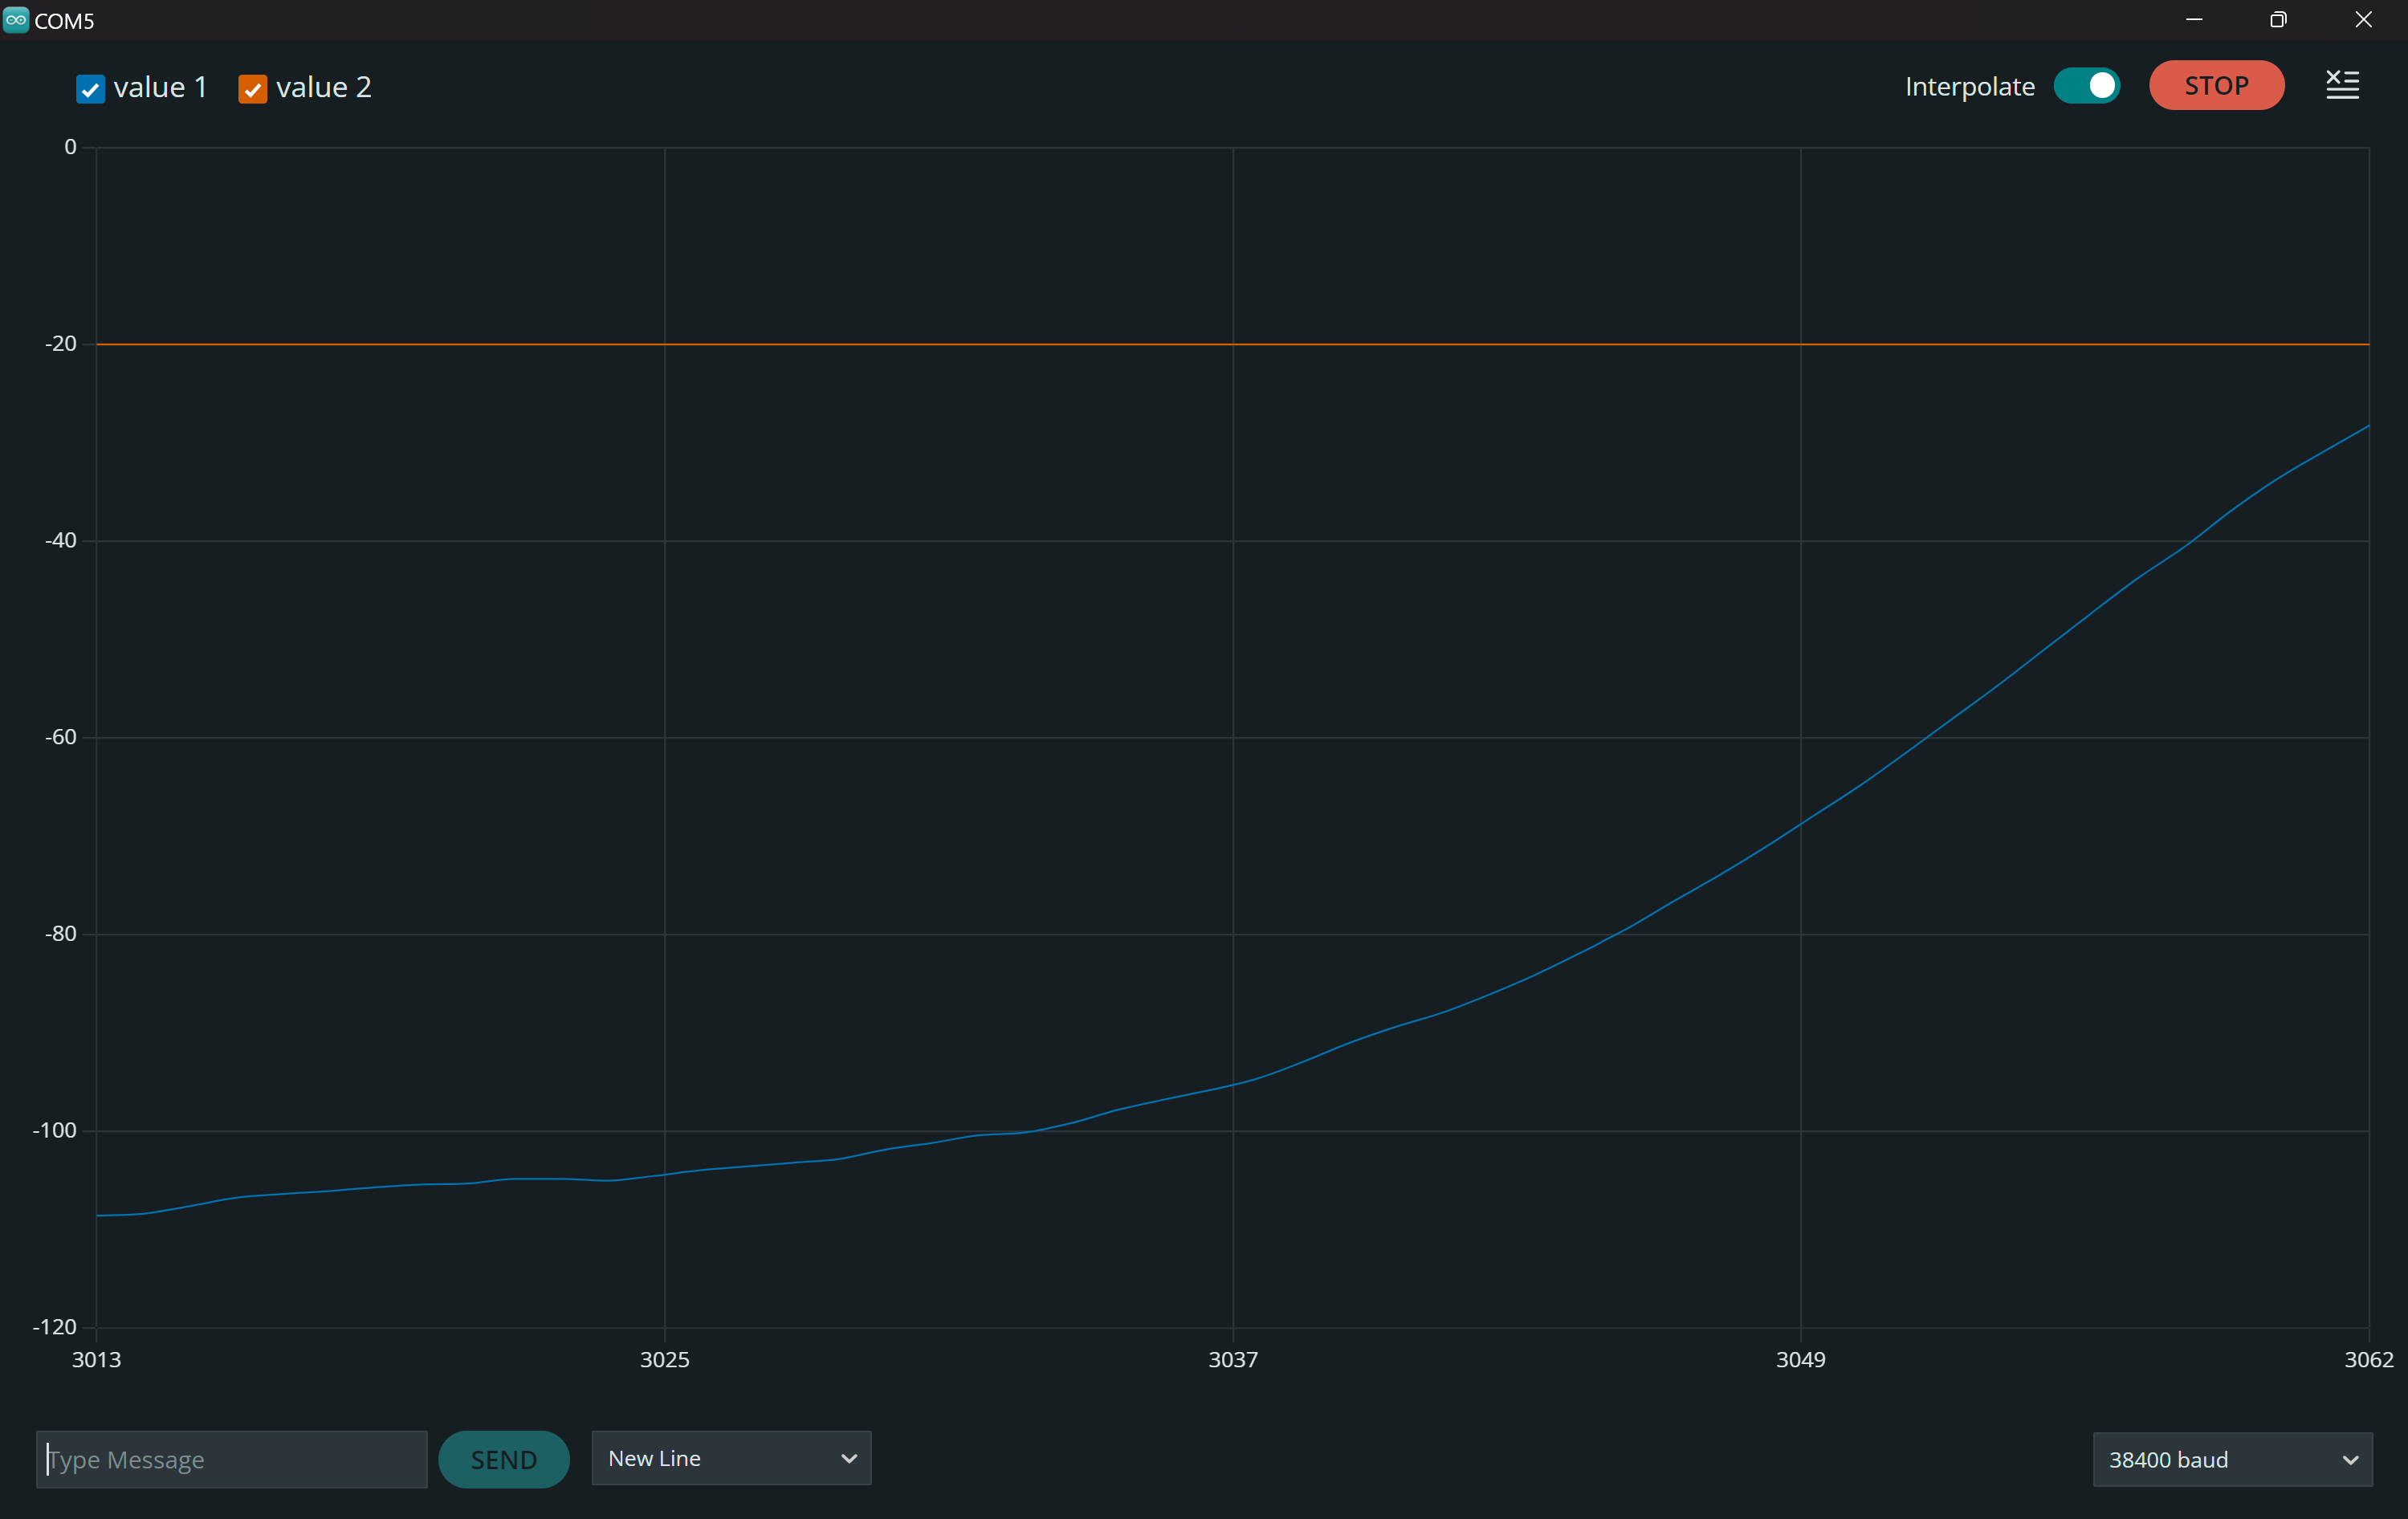
\includegraphics[width=0.95\linewidth]{images/q3/Transient_-20.png}
		\caption{transient response}
    \end{subfigure}
    \begin{subfigure}{.48\textwidth}
        \centering
        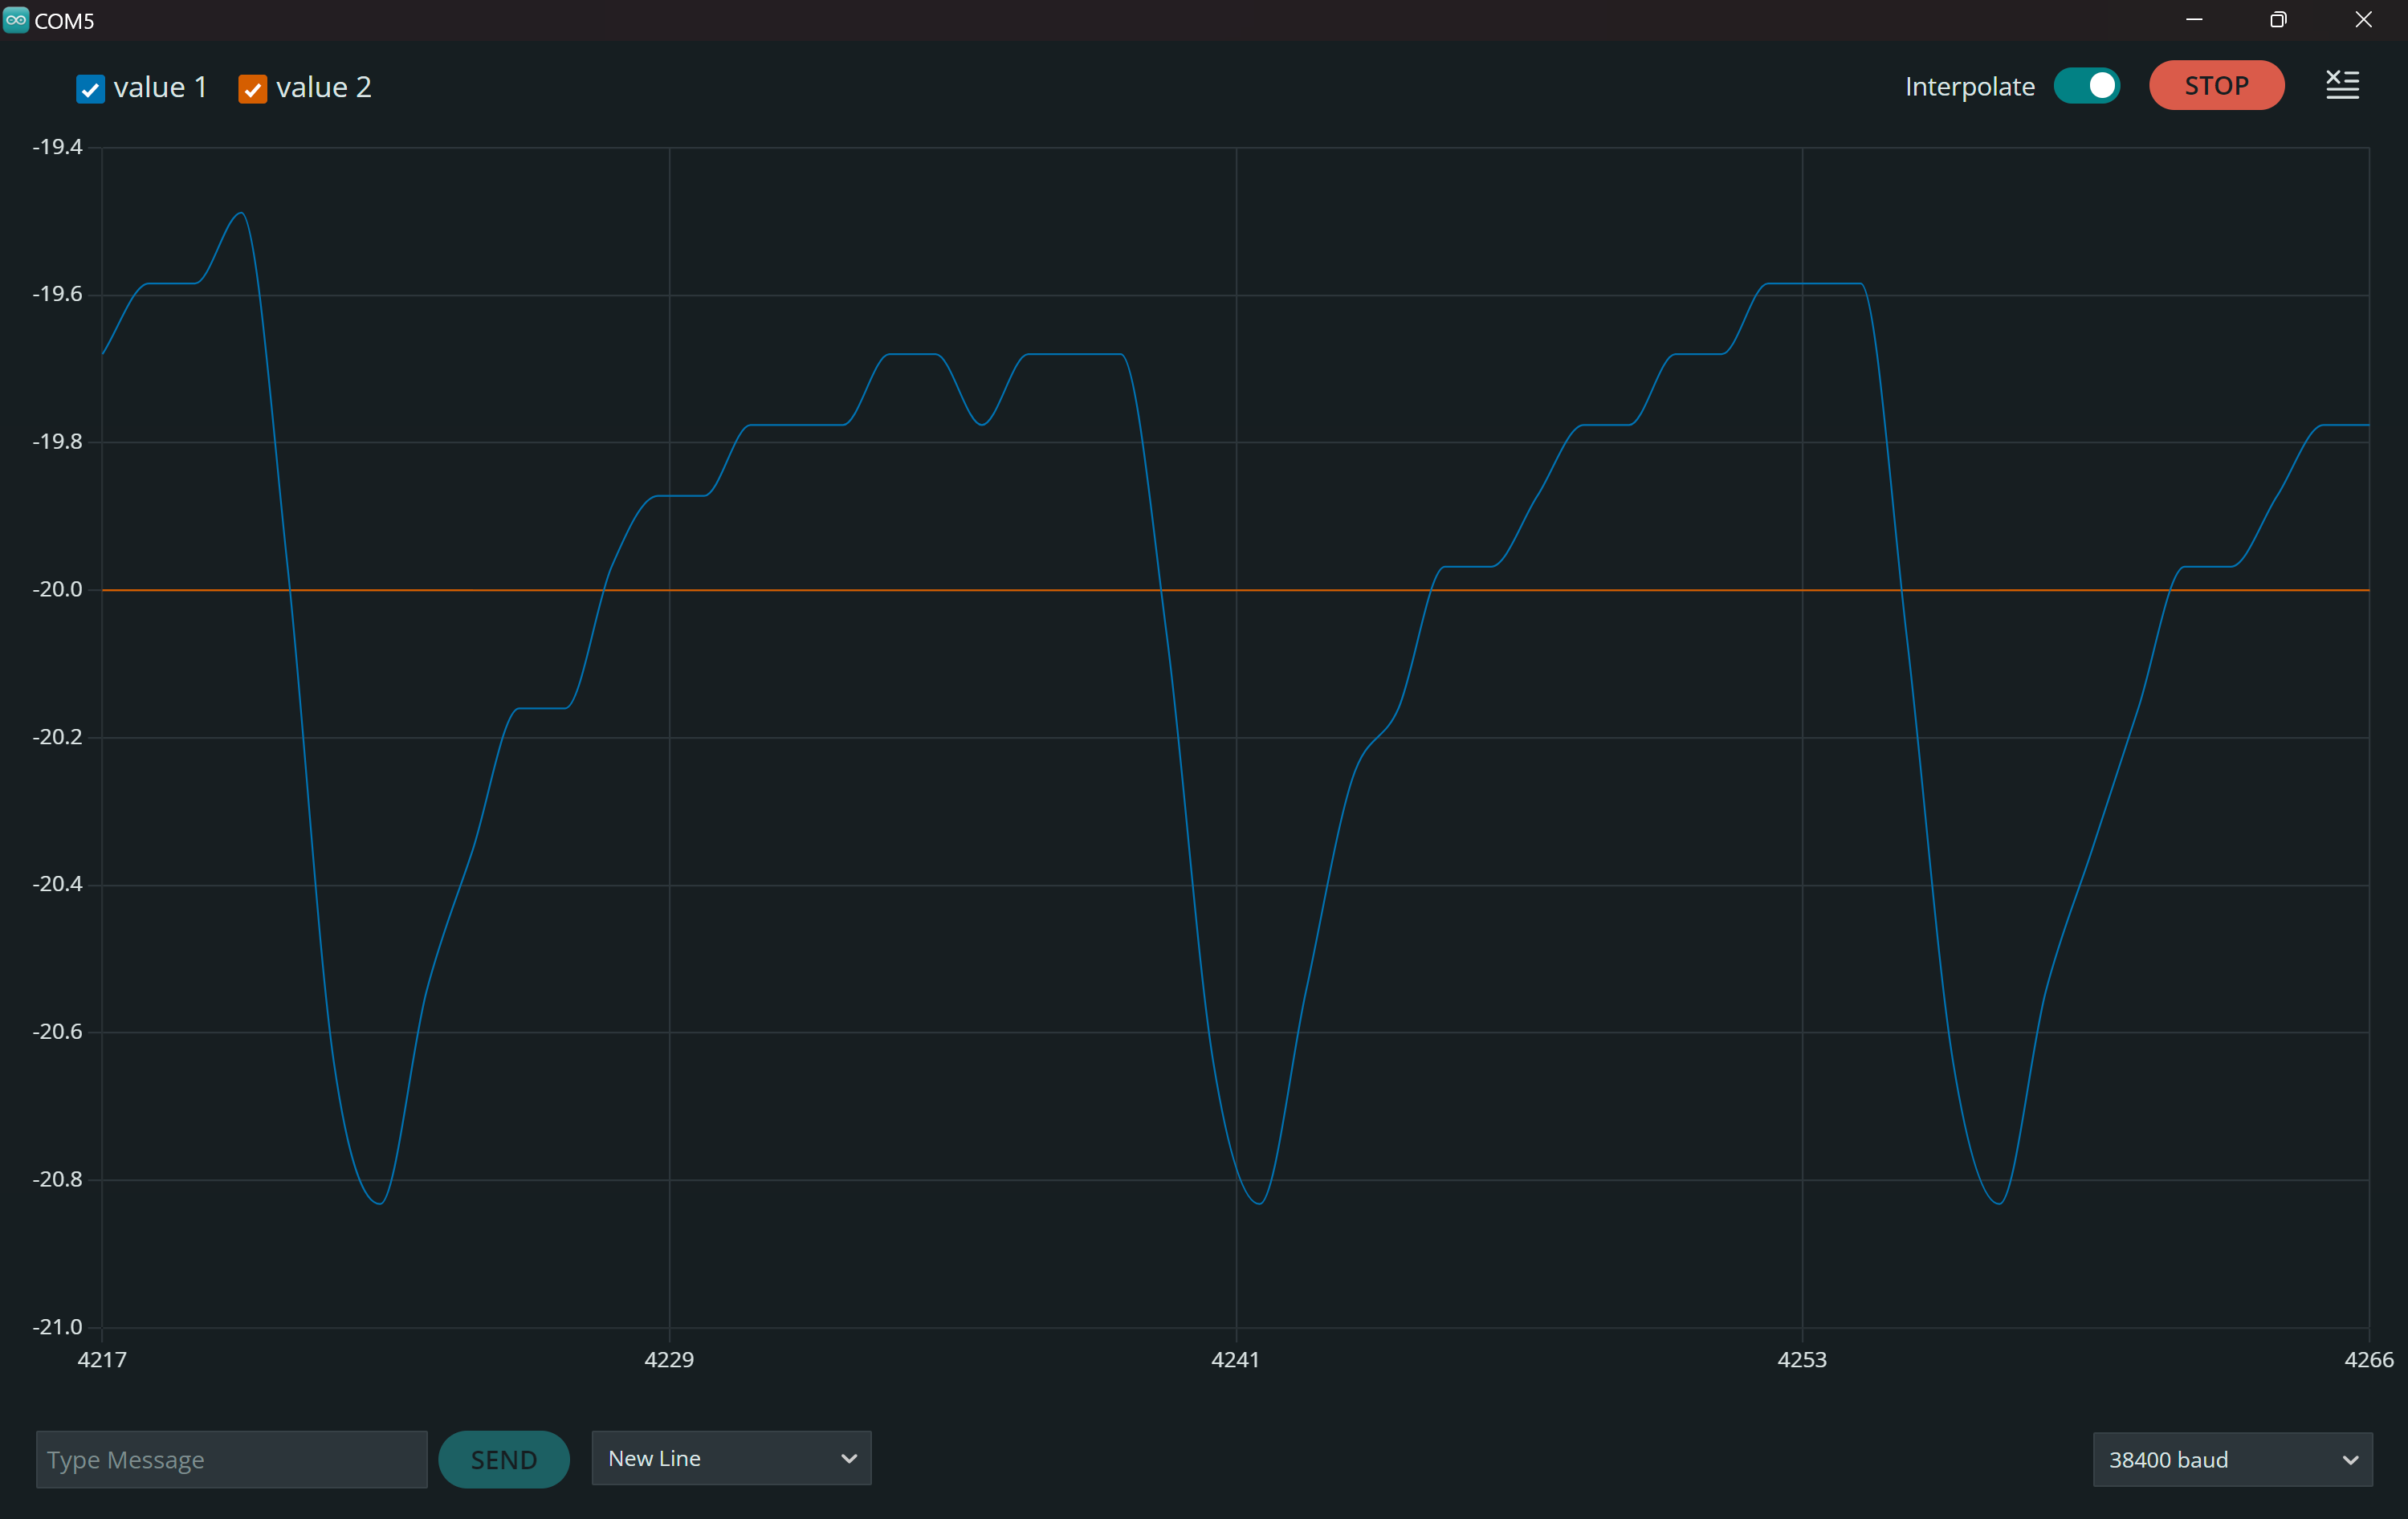
\includegraphics[width=0.95\linewidth]{images/q3/SS_-20.png} 
		\caption{steady state response}
    \end{subfigure}
    \begin{subfigure}{.48\textwidth}
        \centering
        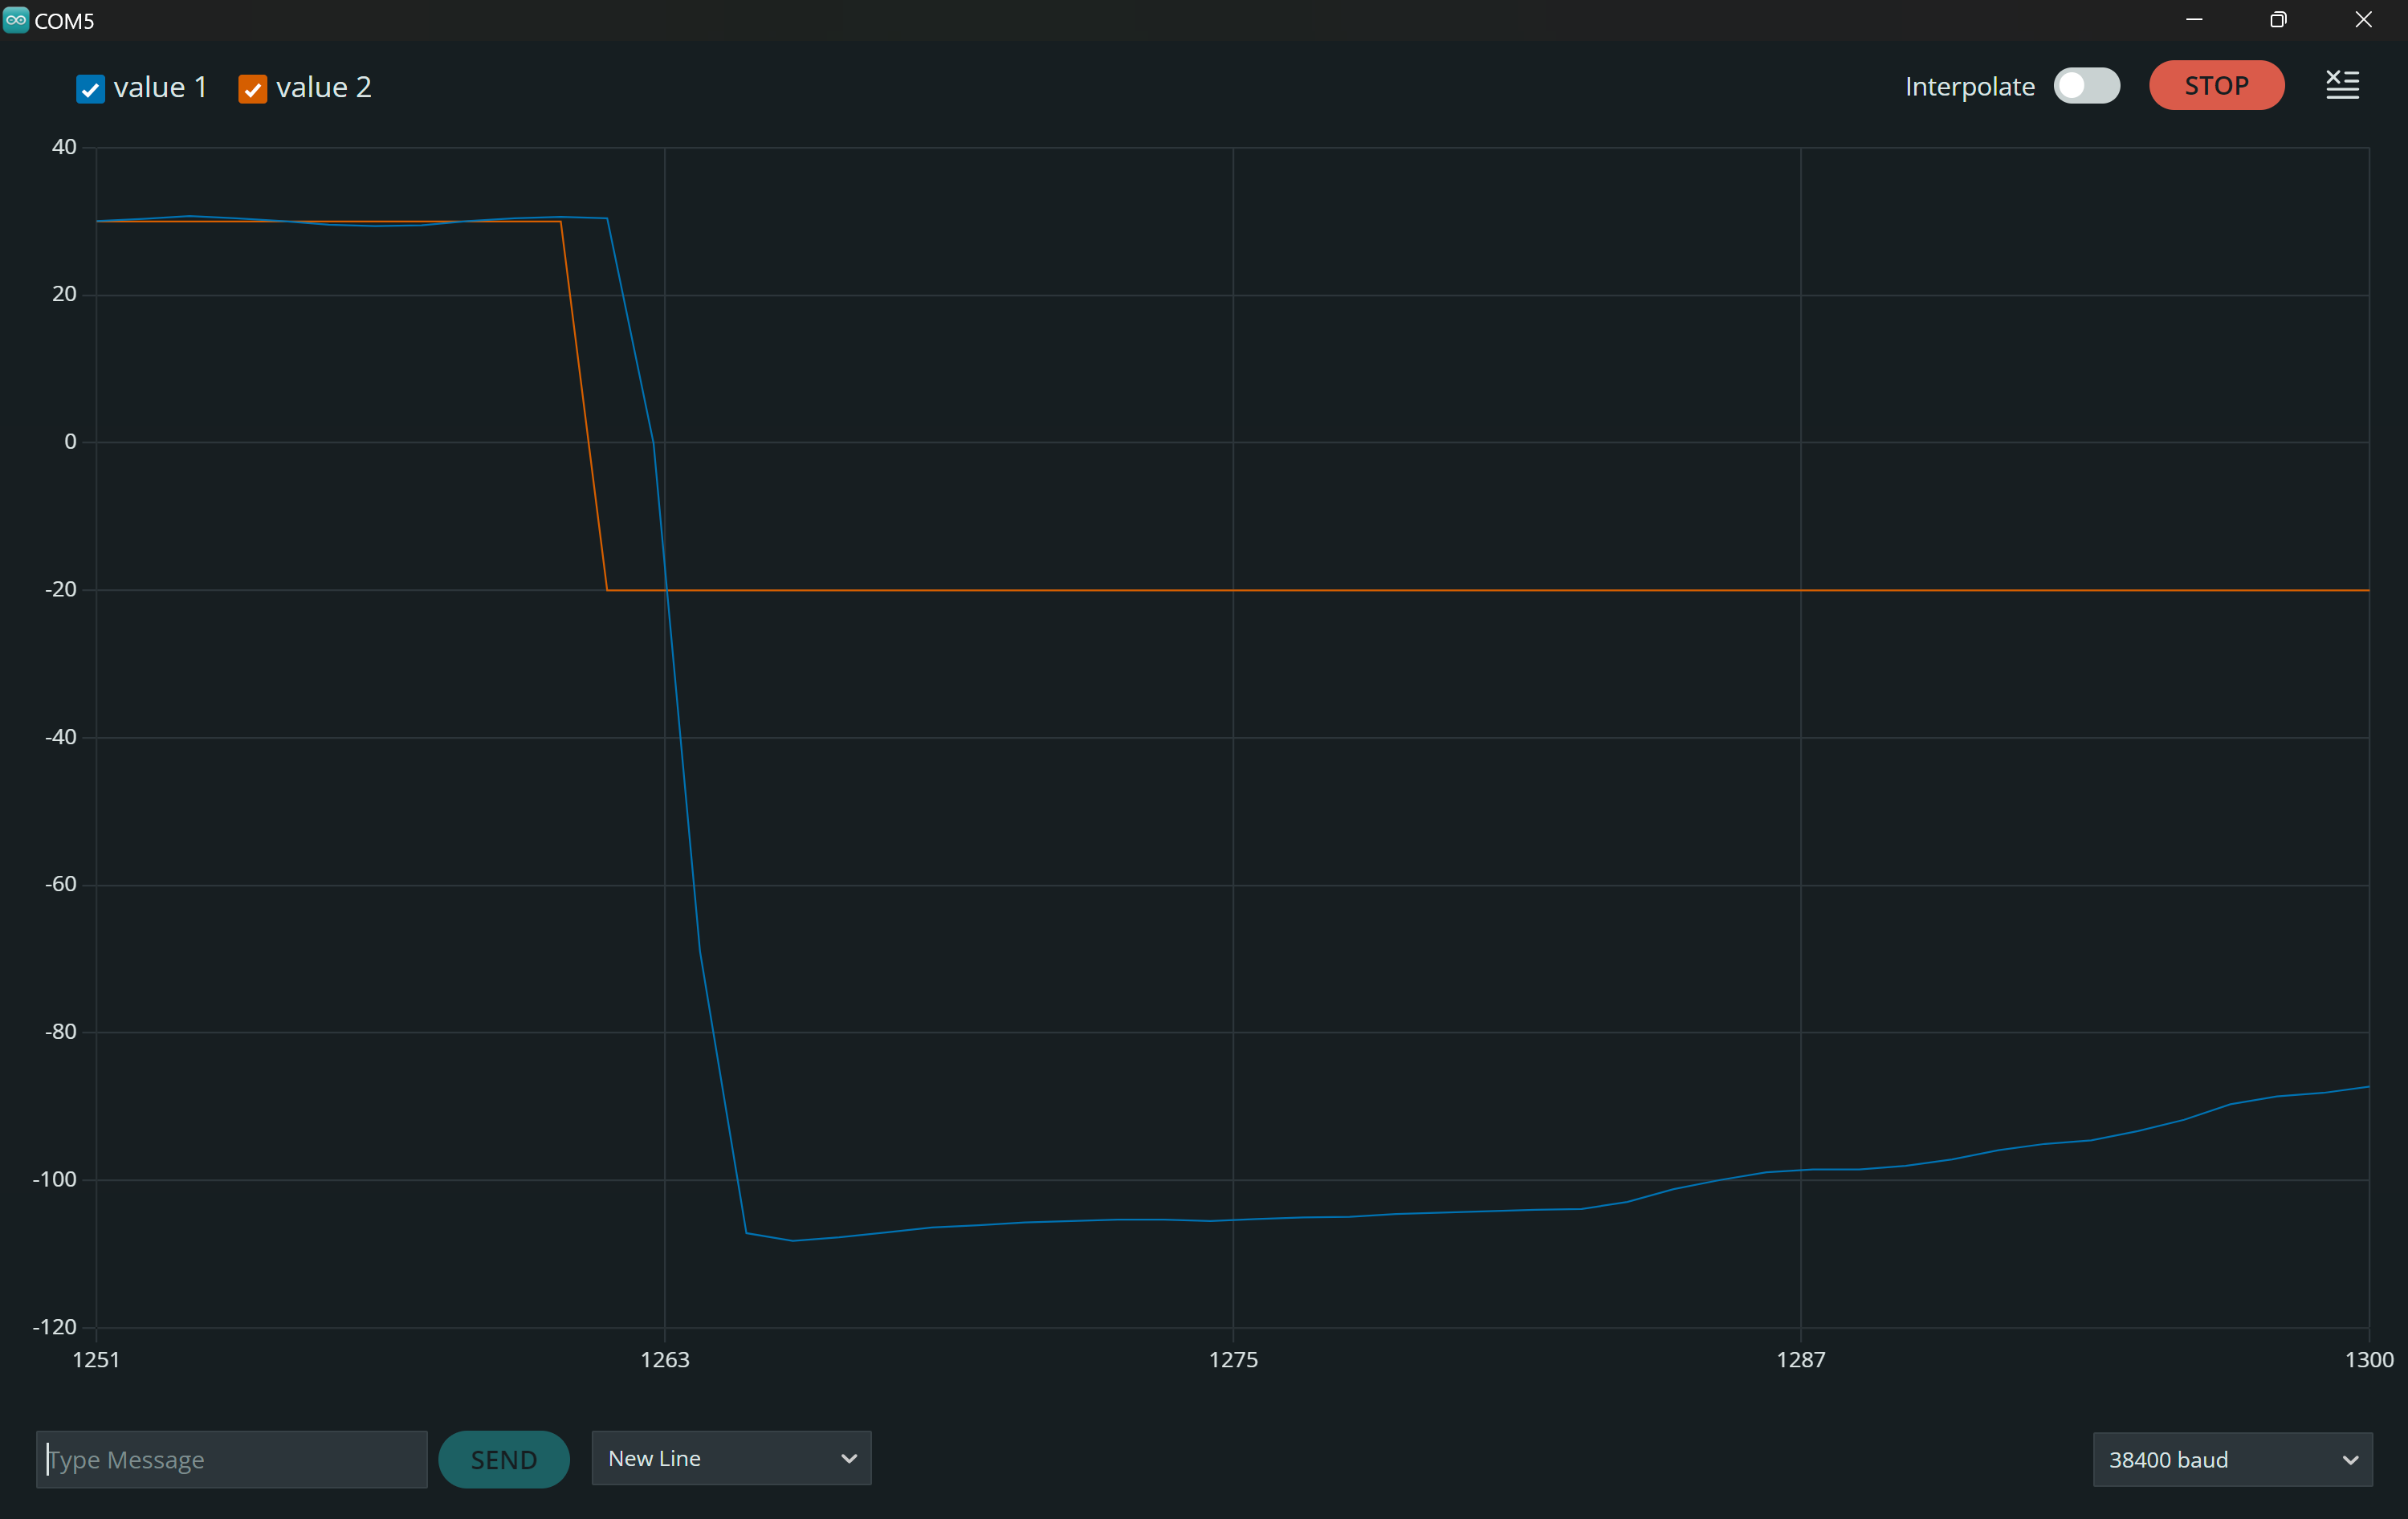
\includegraphics[width=0.95\linewidth]{images/q3/Transition_30_to_-20.png} 
        \caption{transition}
    \end{subfigure}
    \caption{transition from 30 RPM to -20 RPM}
\end{figure}

\subsection{Question 4}
What is the effect of changing PWM frequency on motor speed control for constant PID gain 
values?

\begin{figure}[h]
    \centering
    \begin{subfigure}{.49\textwidth}
        \centering
        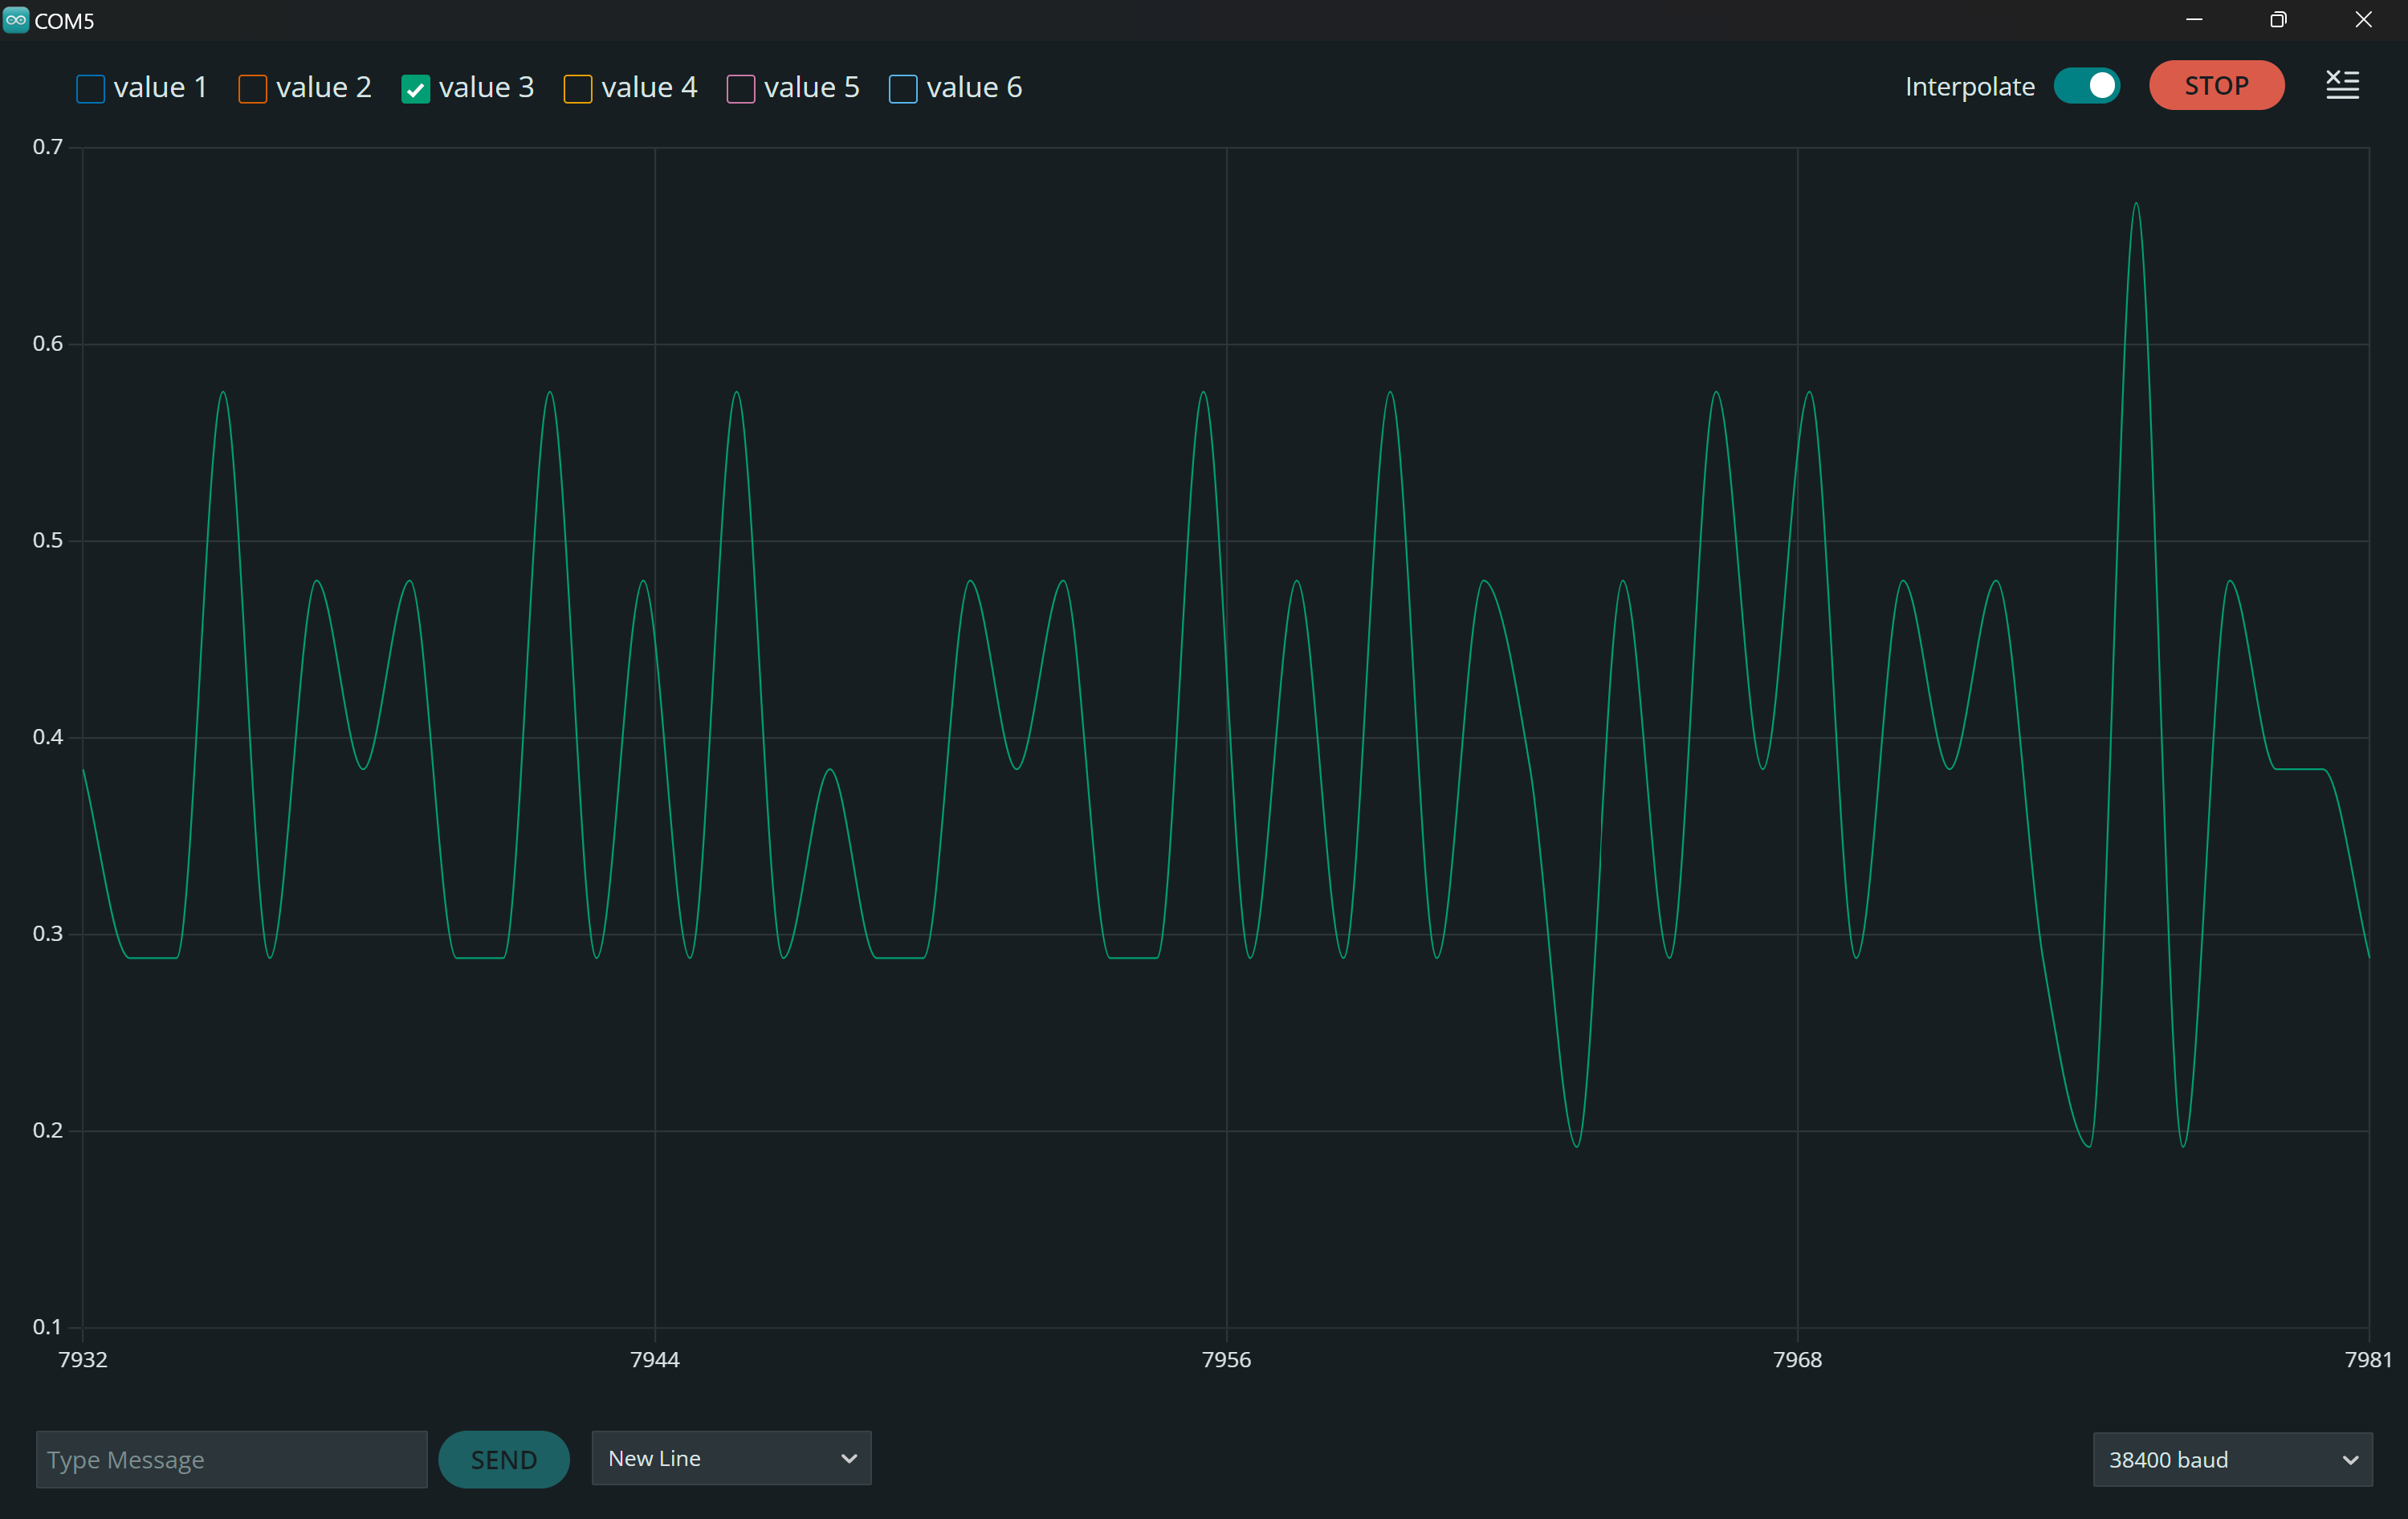
\includegraphics[width=0.95\linewidth]{images/q4/1000Hz.png} 
		\caption{1000 Hz}
    \end{subfigure}
    \begin{subfigure}{.49\textwidth}
        \centering
        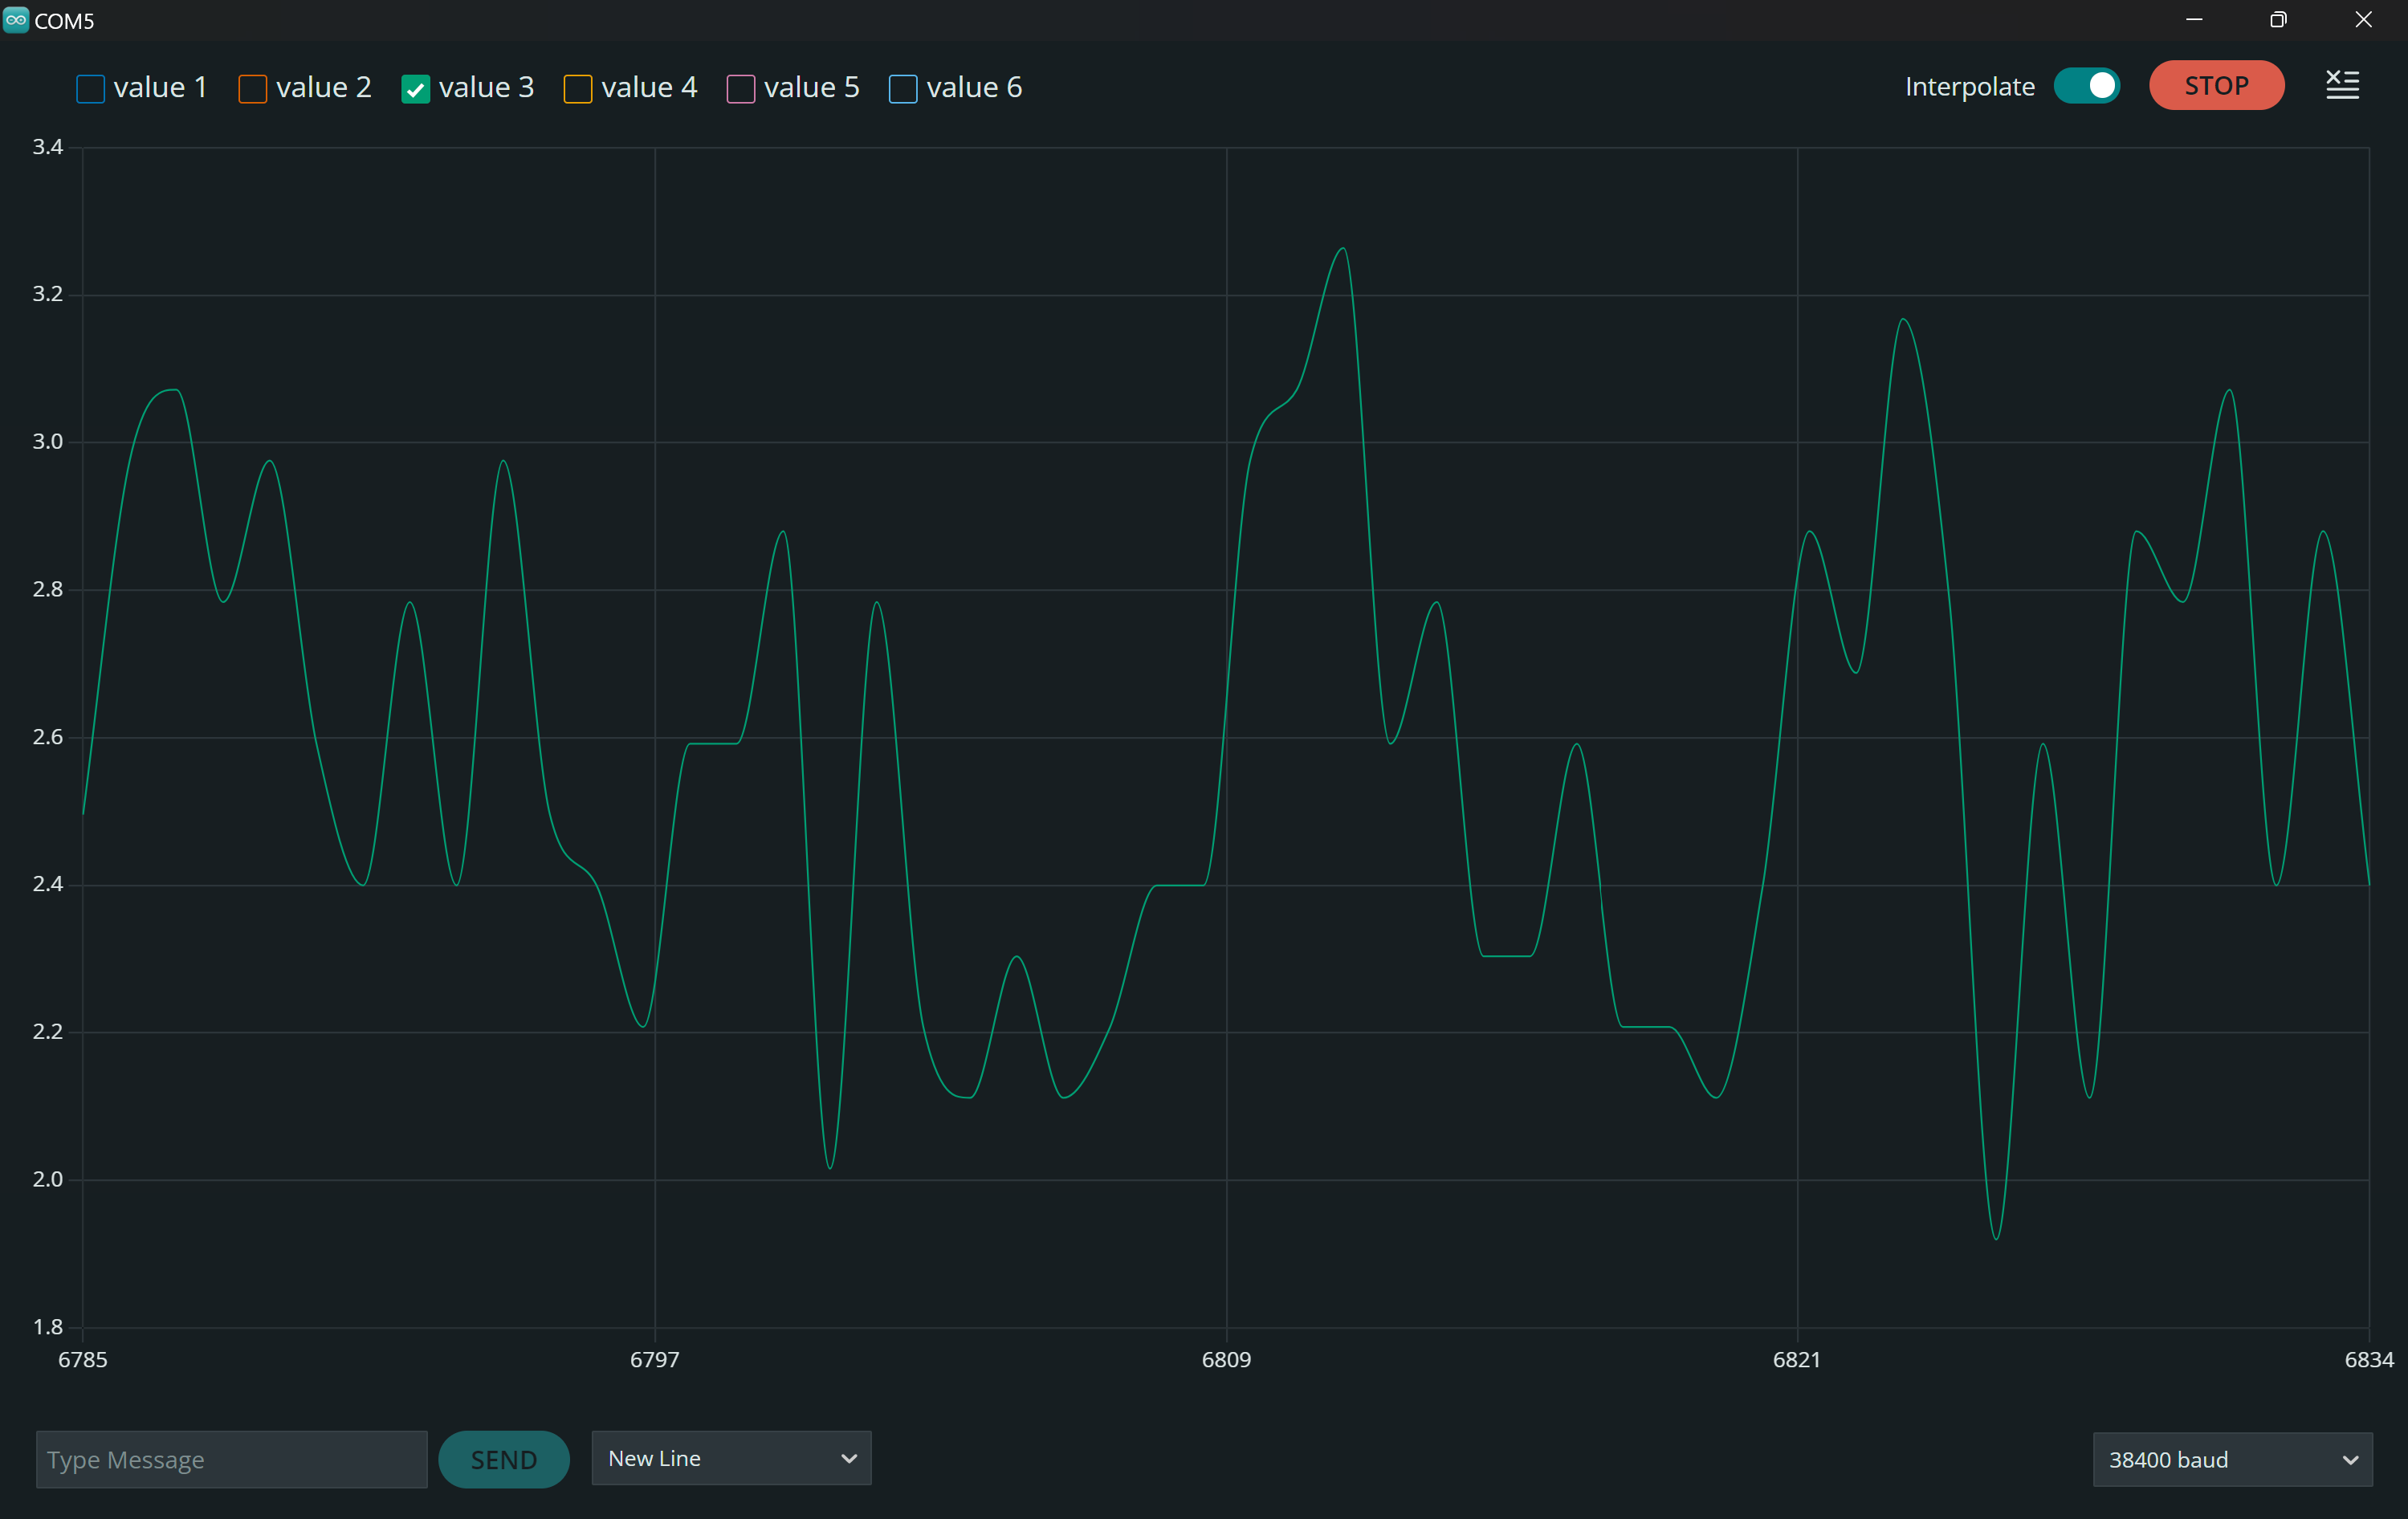
\includegraphics[width=0.95\linewidth]{images/q4/400Hz.png}
		\caption{400 Hz}
    \end{subfigure}
    \begin{subfigure}{.49\textwidth}
        \centering
        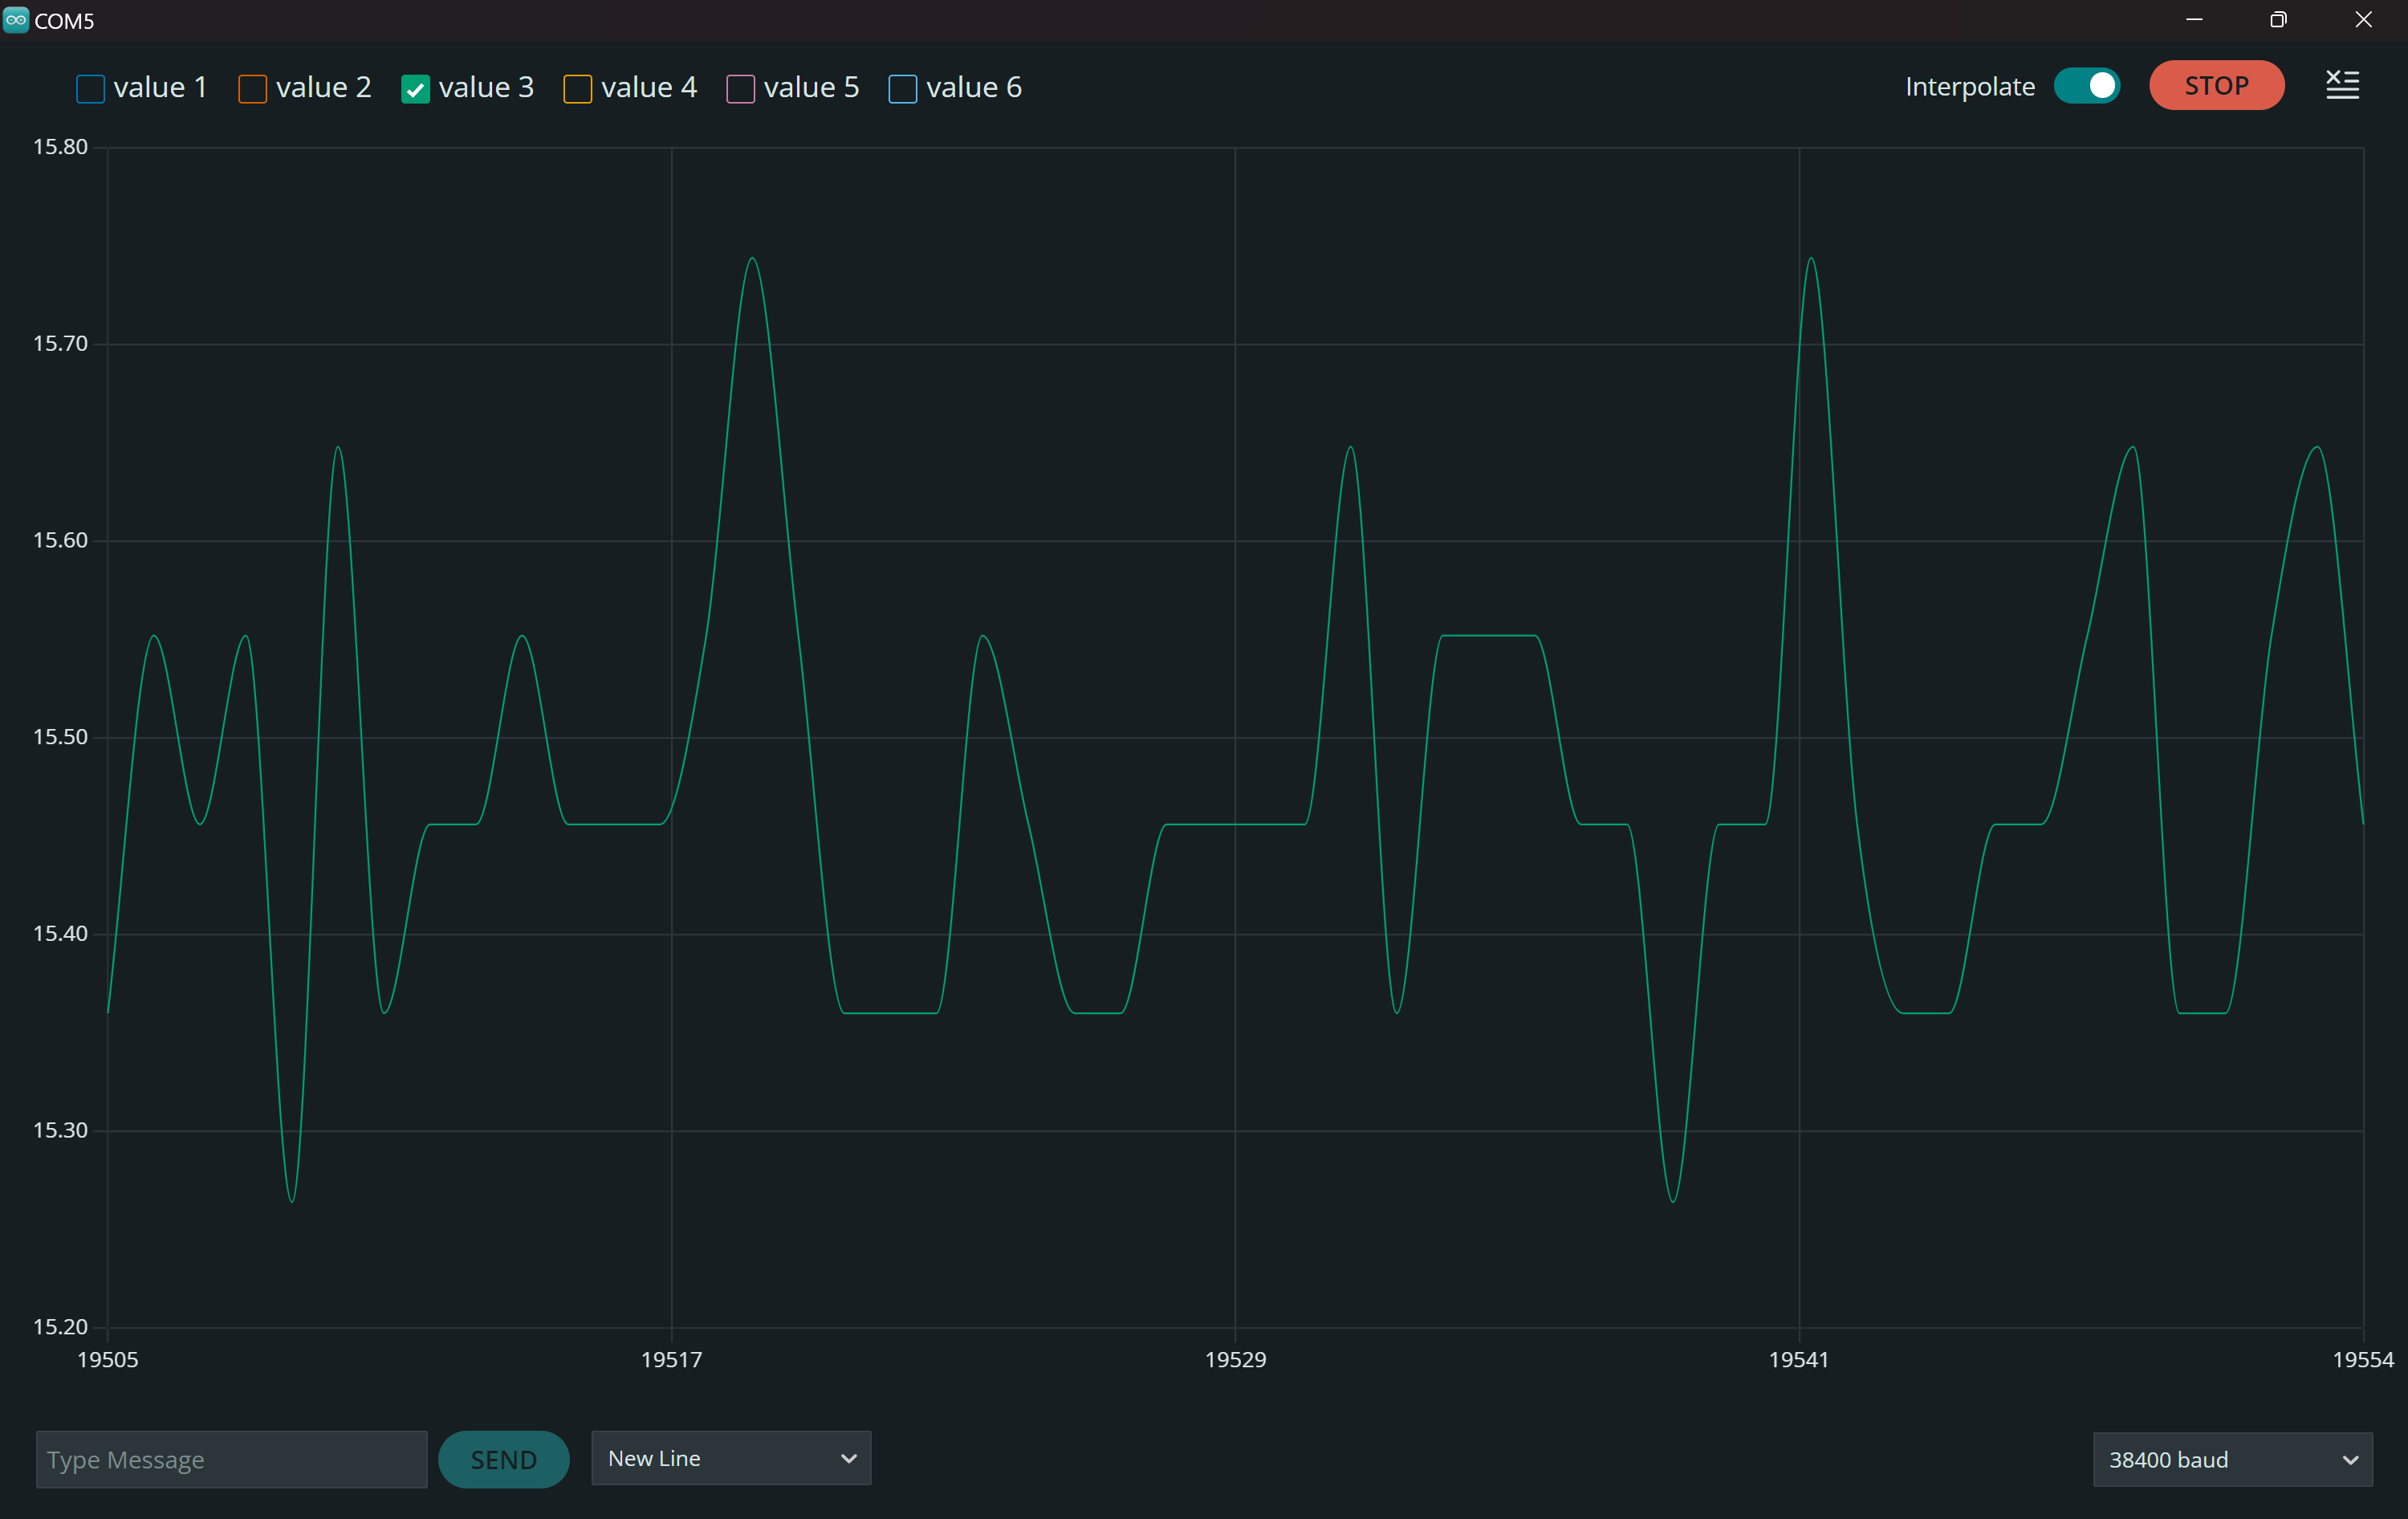
\includegraphics[width=0.95\linewidth]{images/q4/200Hz.png} 
        \caption{200 Hz}
    \end{subfigure}
	\begin{subfigure}{.49\textwidth}
        \centering
        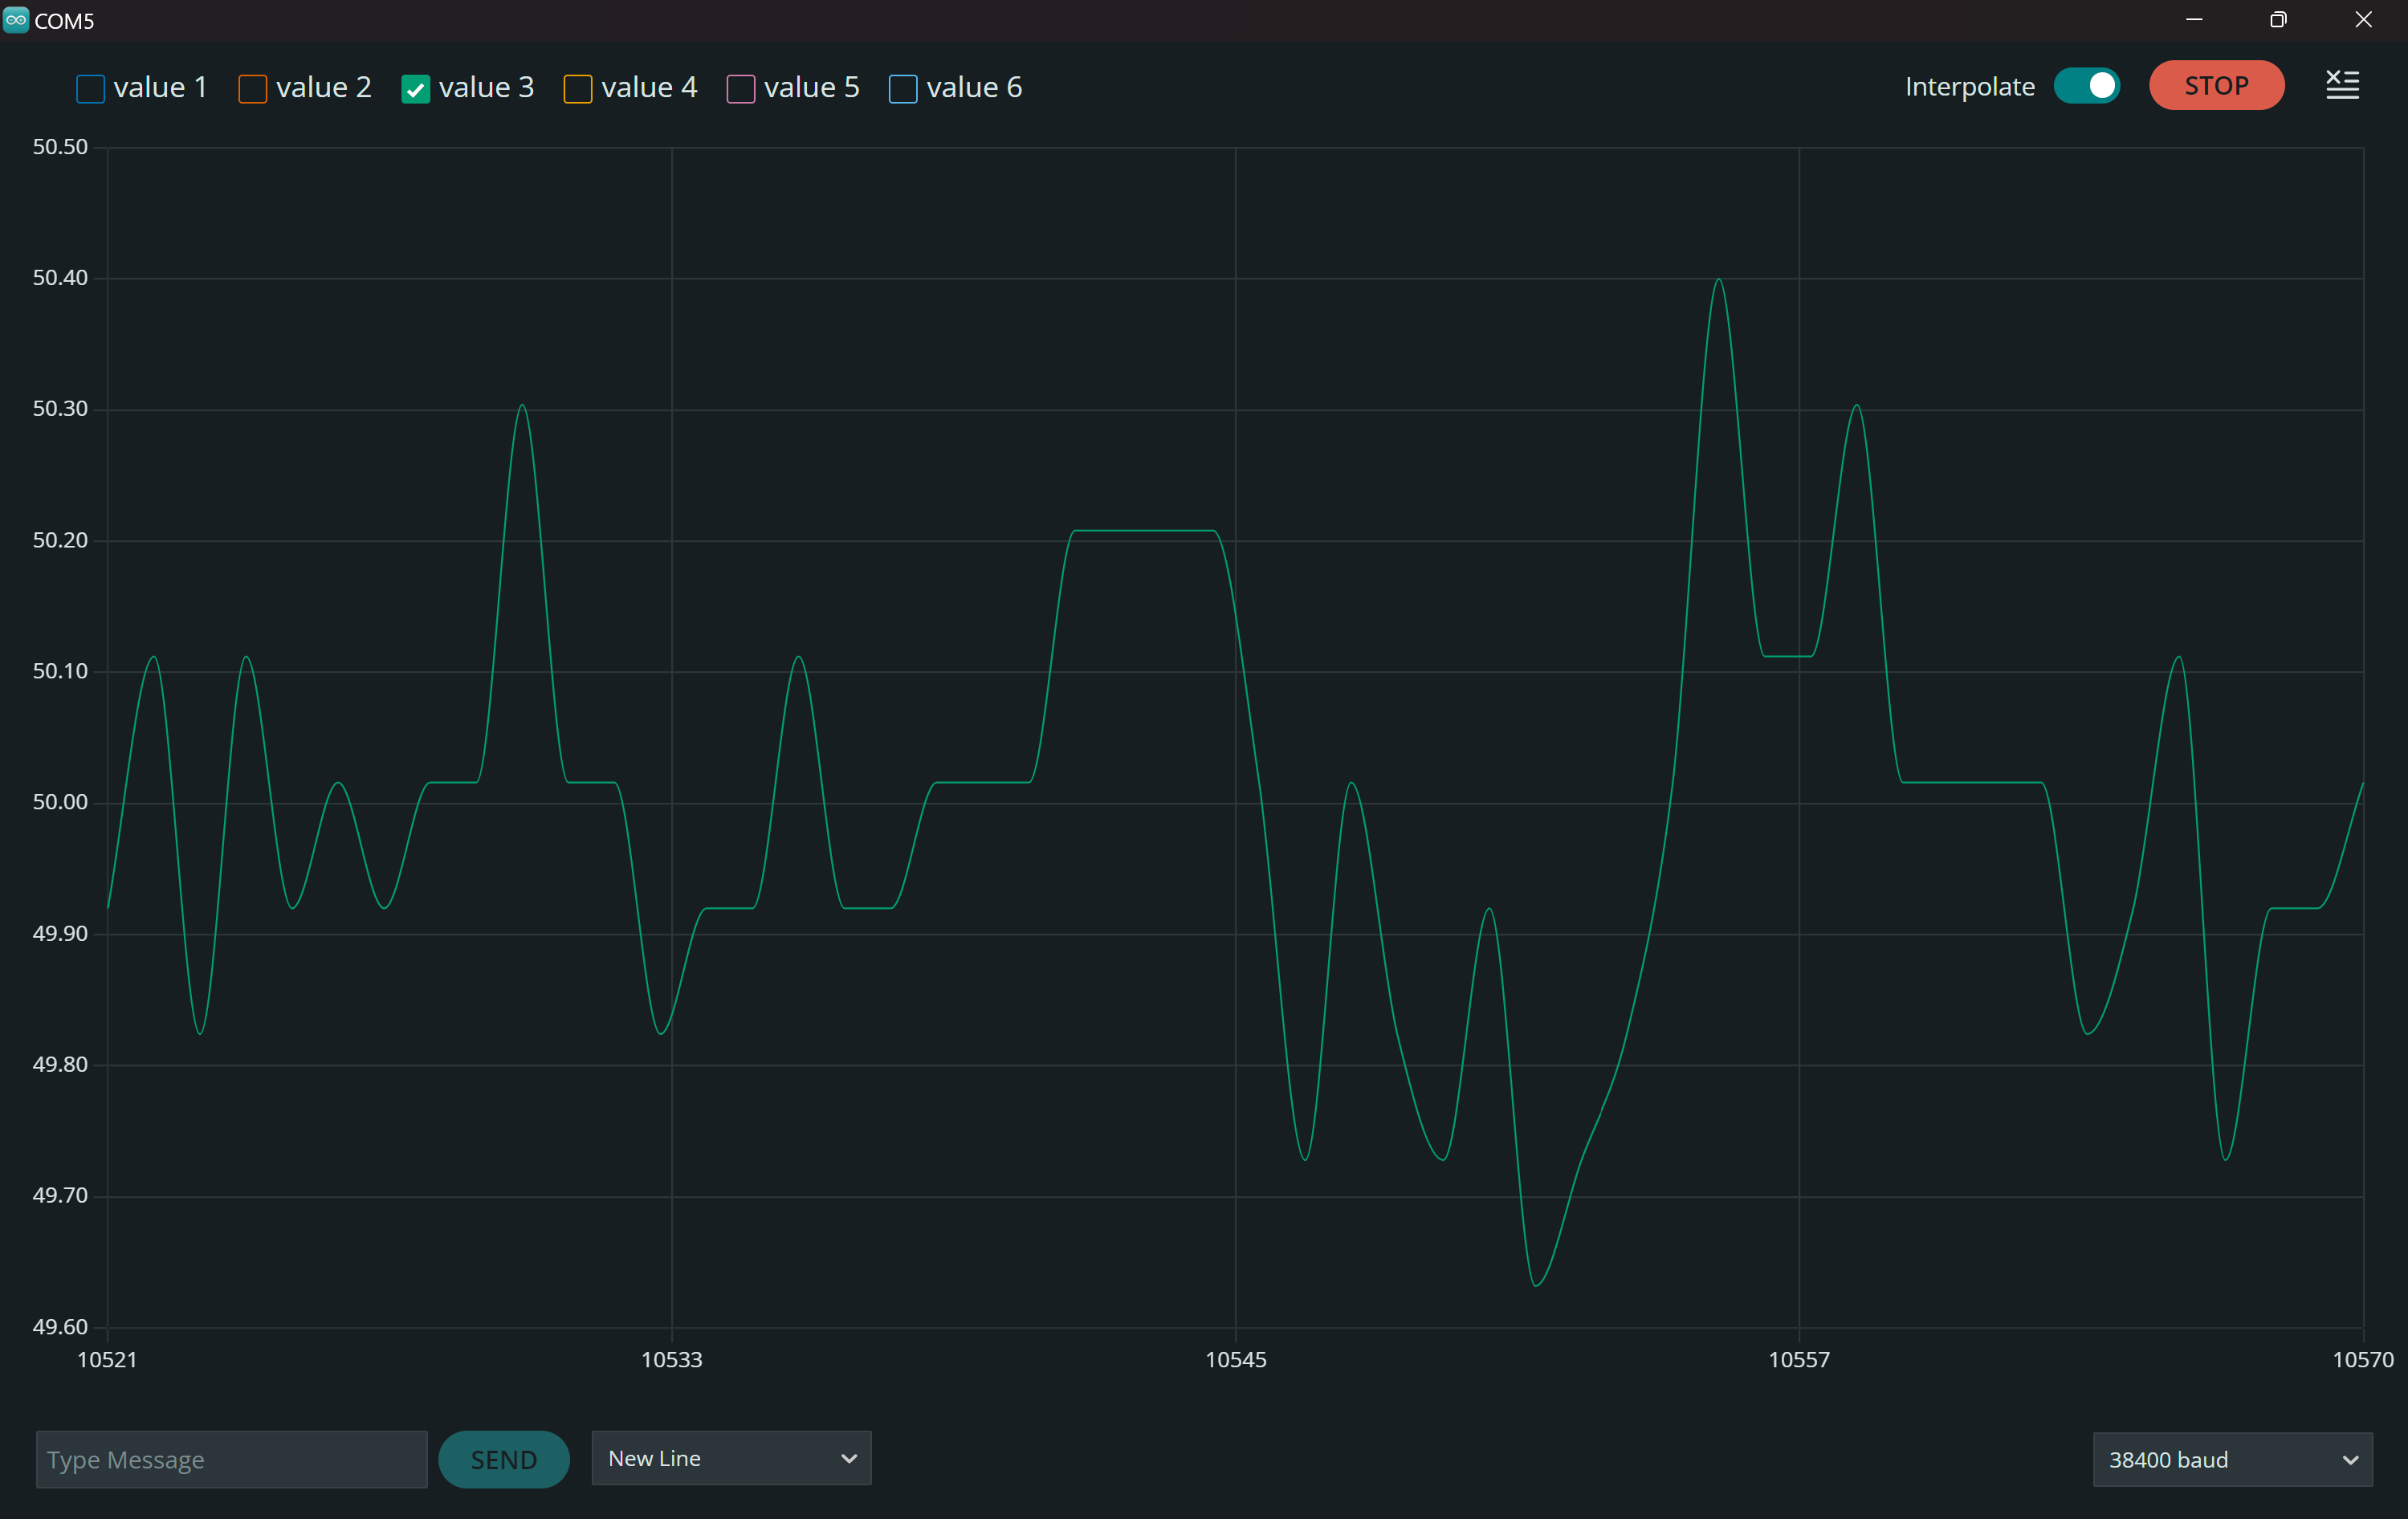
\includegraphics[width=0.95\linewidth]{images/q4/100Hz.png}
		\caption{100 Hz}
    \end{subfigure}
	\begin{subfigure}{.49\textwidth}
        \centering
        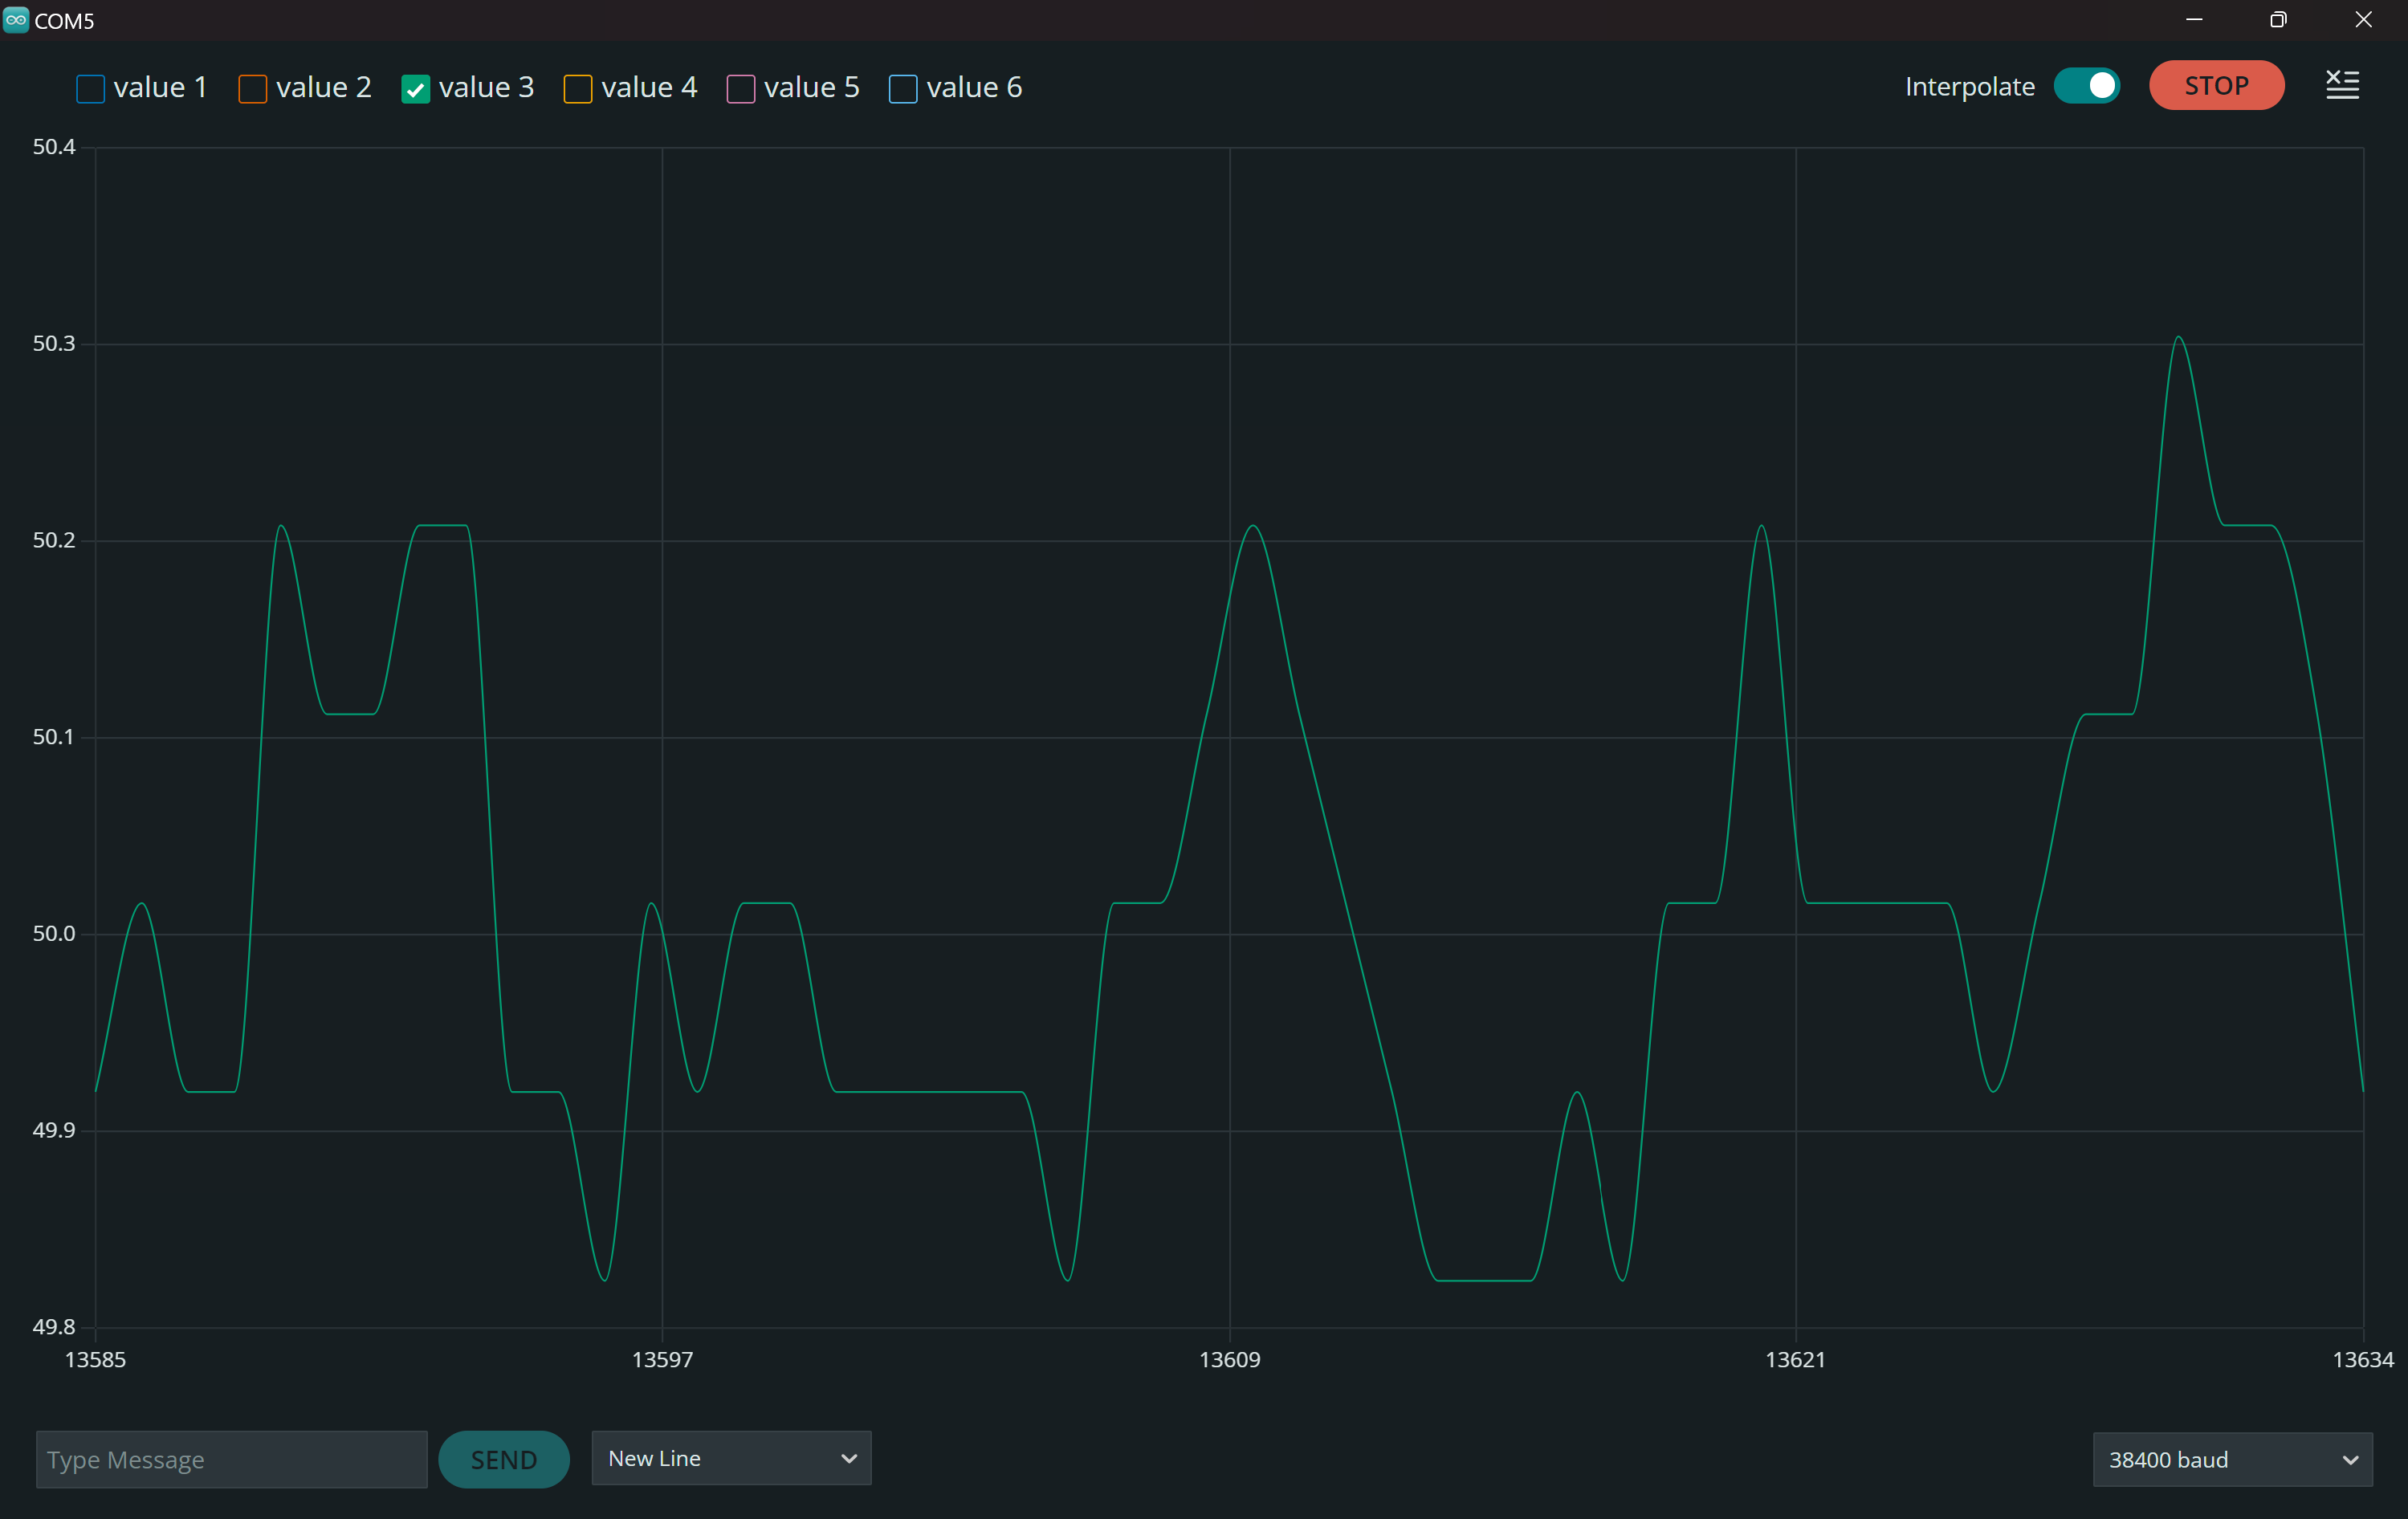
\includegraphics[width=0.95\linewidth]{images/q4/75Hz.png}
		\caption{75 Hz}
    \end{subfigure}
    \begin{subfigure}{.49\textwidth}
        \centering
        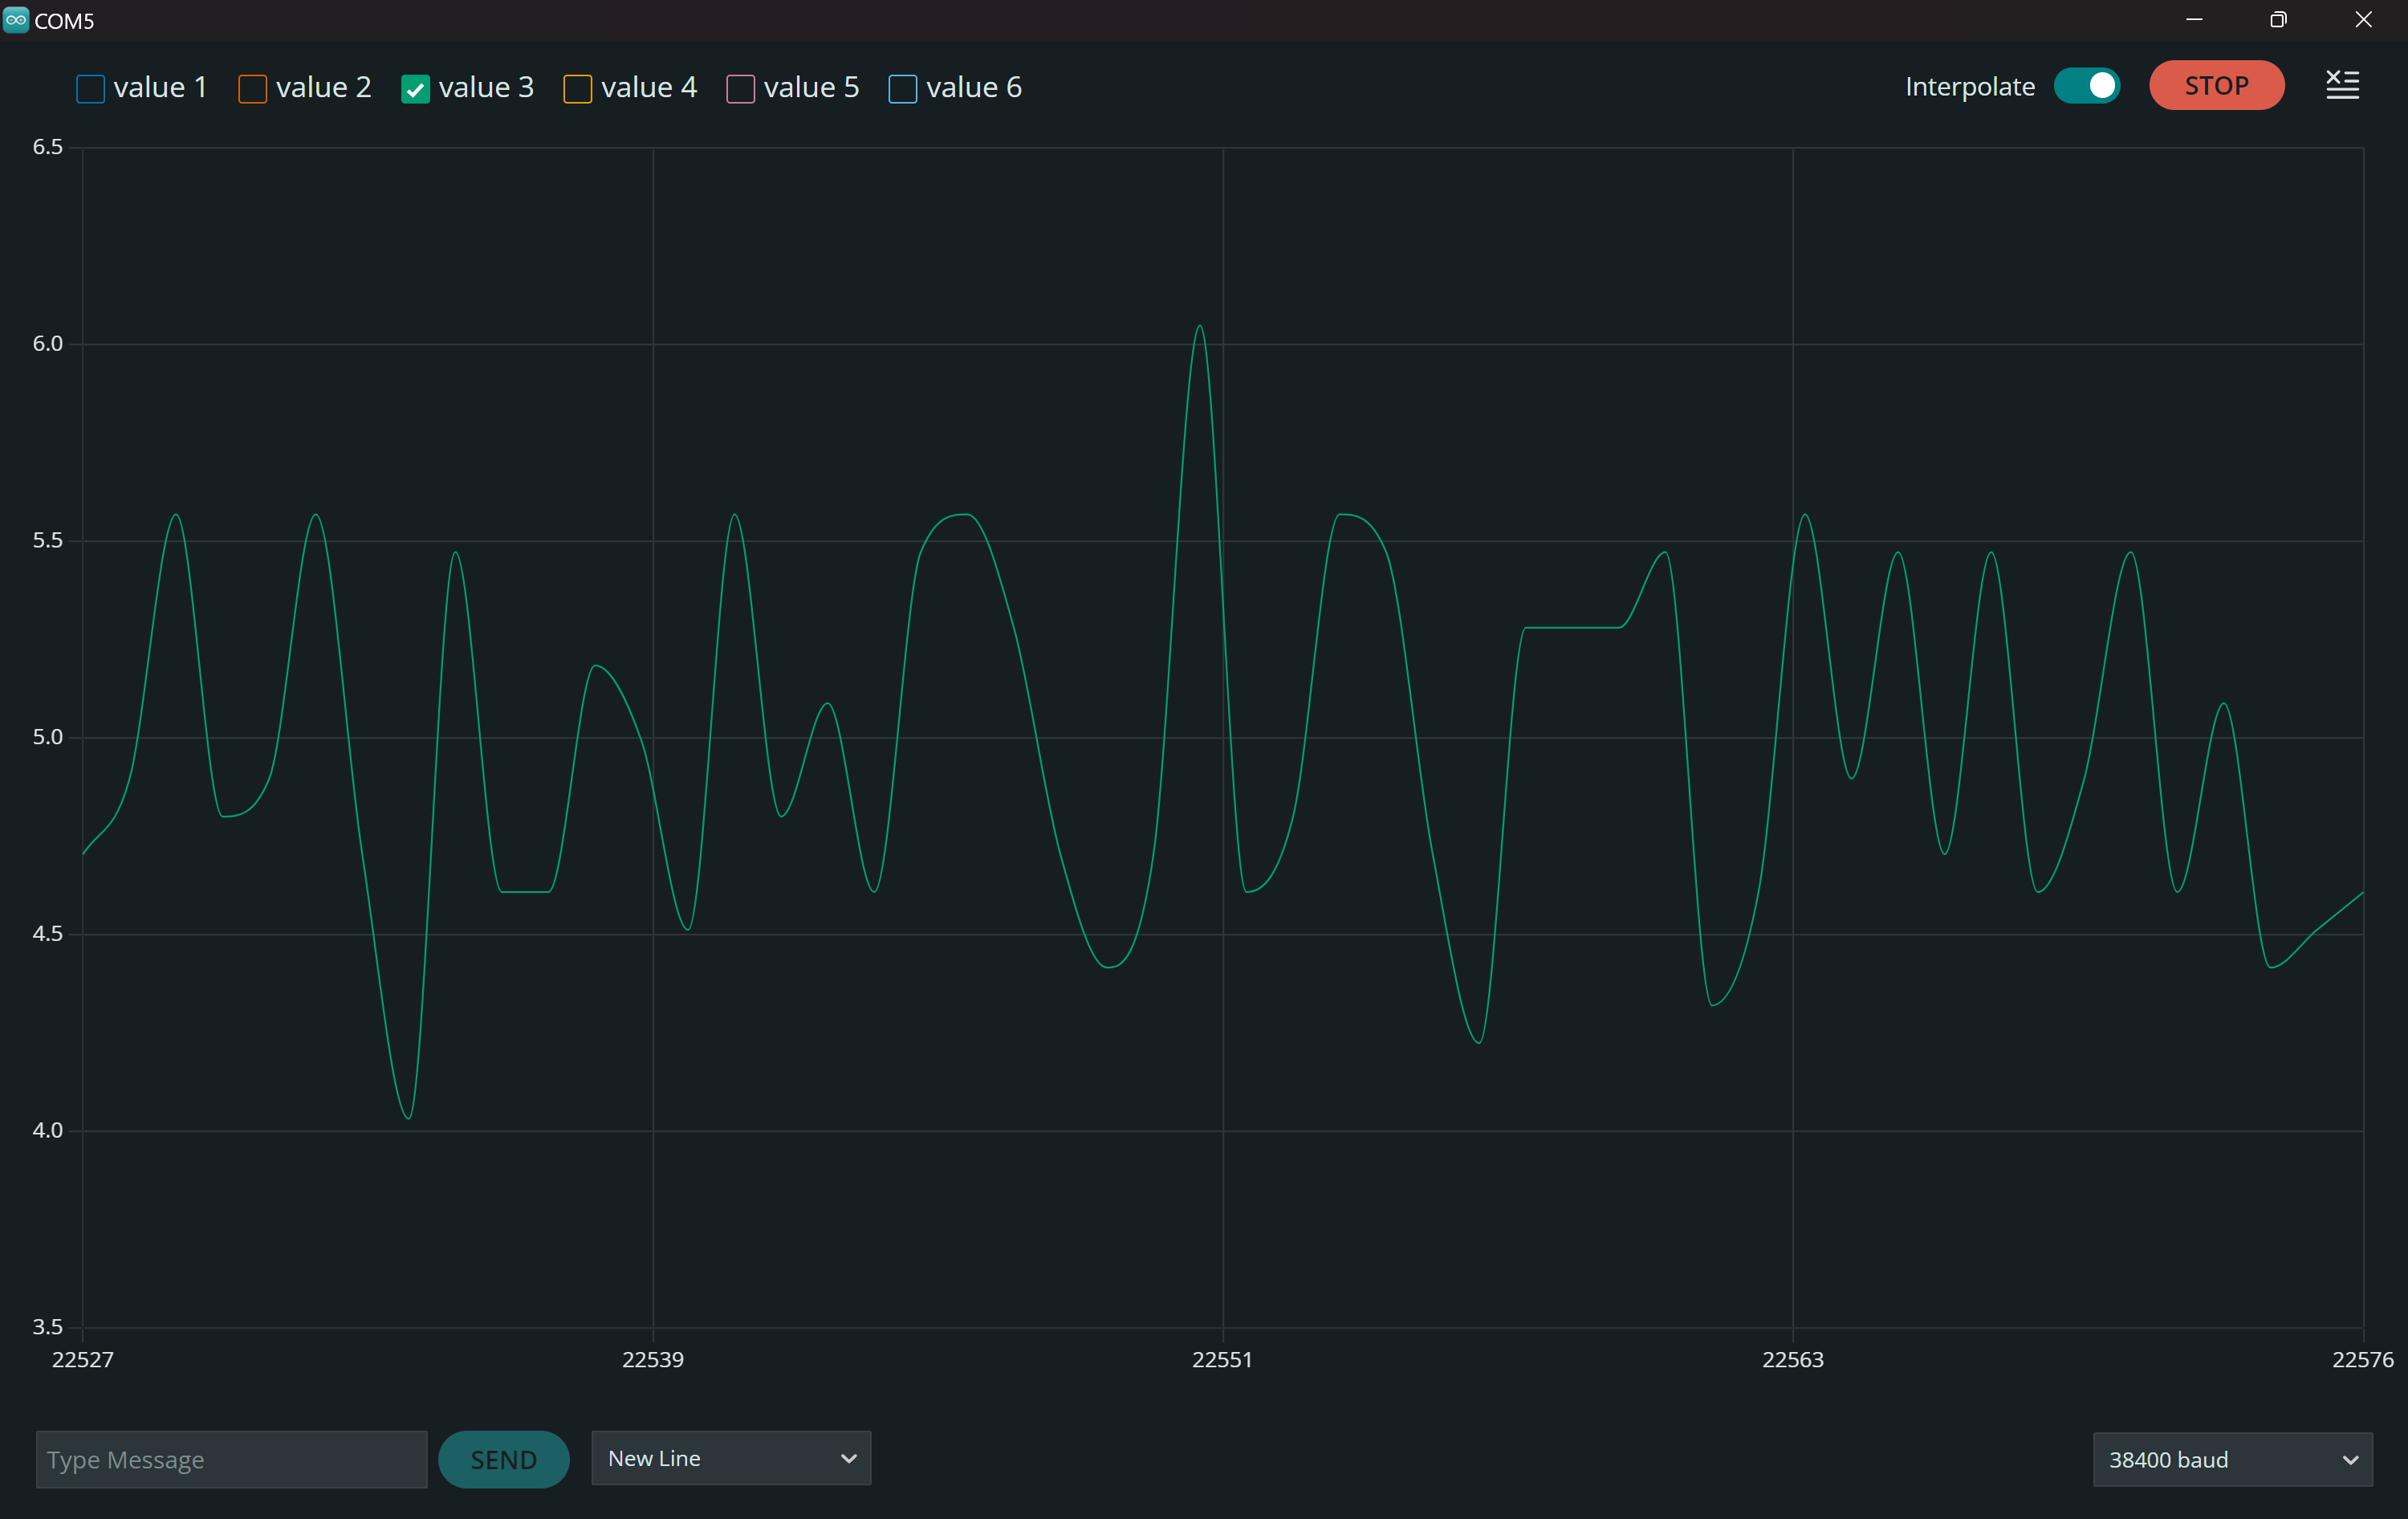
\includegraphics[width=0.95\linewidth]{images/q4/50Hz.png} 
		\caption{50 Hz}
    \end{subfigure}
    \begin{subfigure}{.49\textwidth}
        \centering
        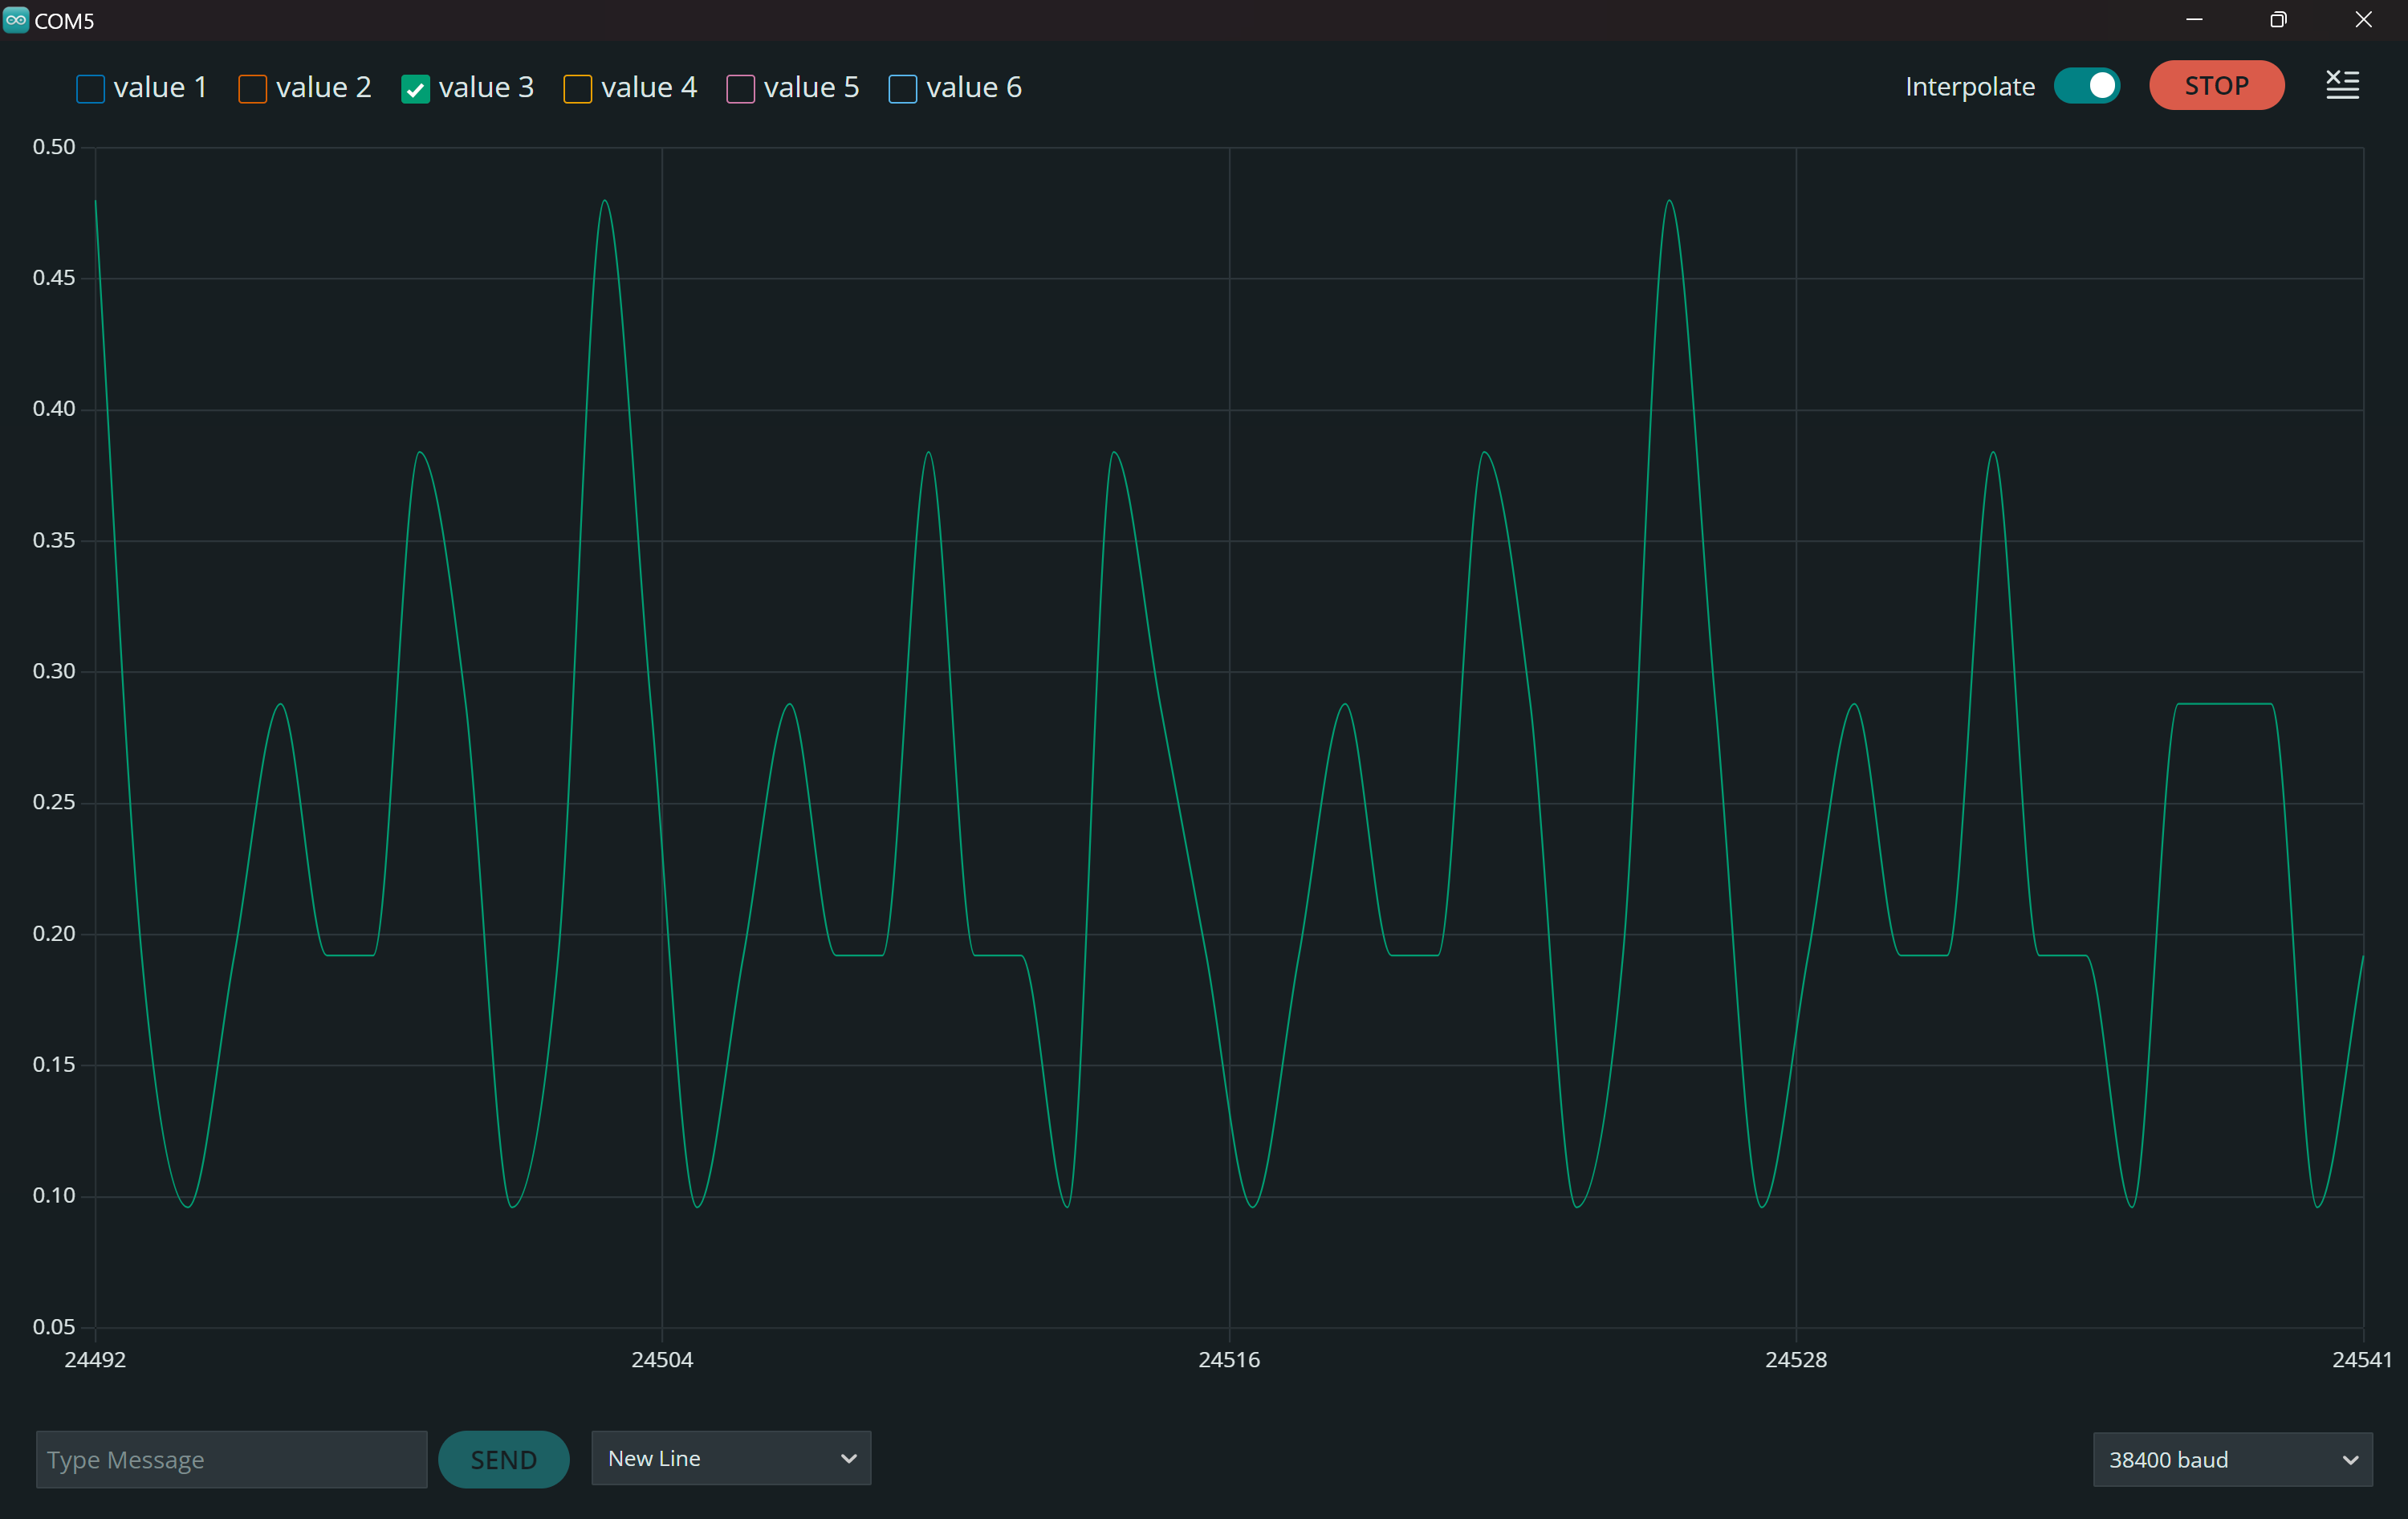
\includegraphics[width=0.95\linewidth]{images/q4/20Hz.png} 
		\caption{20 Hz}
    \end{subfigure}
    \caption{transient responses serial plots}
\end{figure}

\end{document}